\documentclass[a4paper, 12pt]{report}

\usepackage[utf8]{inputenc}
\usepackage{amsmath}
\usepackage{amssymb}
\usepackage[super]{natbib}
\usepackage{graphicx}
\usepackage{epstopdf}
\usepackage[margin=1.0in]{geometry}
\usepackage{dcolumn}
\usepackage{appendix}
\usepackage{fixltx2e}	
\usepackage{natbib}
\usepackage{subfig}
\usepackage{float}
\usepackage{url}
\usepackage[nonumberlist]{glossaries}
\usepackage{setspace}
\usepackage[usenames, dvipsnames]{color}
\usepackage{titlepic}
\usepackage{standalone}
\usepackage{listings}

\onehalfspacing
\renewcommand{\abstractname}{Abstract of Non-linear Relationships in Big Data}
\makeglossaries
 %   \bibpunct[, ]{(}{)}{;}{a}{,}{,}

\title{Non-linear Relationships in Big Data}
\author{Julian Roche  \\  \\ Submitted in partial fulfilment of the requirements for the MSc in Statistics \\ \\ School of Mathematics and Statistics}
\date{September 2015}

\newglossaryentry{A}
{
  name=A,
  description={A measure of association that generalises $R^2$ to handle non-linear associations. It is implemted in the R $matie$ package.}
}

\newglossaryentry{MATIE}
{
  name=MATIE,
  description={Measuring Association and Testing Independence Efficiently, an implementation in R of $A$}
}

\newglossaryentry{FDR}
{
  name=FDR,
  description={False Discovery Rate. A technique for limiting Type I errors in hypothesis tests}
}

\newglossaryentry{GAM}
{
  name=GAM,
  description={Generalised Additive Model}
}

\newglossaryentry{MARS}
{
  name=MARS,
  description={Multiple Adaptive Regression Splines}
}

\newglossaryentry{FDA}
{
  name=FDA,
  description={Flexible Discriminant Analysis}
}

\newglossaryentry{DE}
{
  name=DE,
  description={A gene which is differentially expressed}
}

\newglossaryentry{RV}
{
  name=r.v.,
  description={Random Variable}
}


\newglossaryentry{Equatibility}
{
  name=Equatibility,
  description={The ability to score equally, noisy relationships of different types}
}

\newglossaryentry{Power}
{
  name=Power,
  description={The ability to correctly reject the null hypothesis when it is false}
}


\newglossaryentry{MIC}
{
  name=MIC,
  description={Maximal Information Coefficient. An information theoretic measure of association}
}

\newglossaryentry{dcor}
{
  name=dcor,
  description={Distance correlation. A statistical measure of distance based on functions of distances between statistical observations in metric spaces}
}

\newglossaryentry{MDS}
{
  name=MDS,
  description={Multidimensional Scaling}
}

\newglossaryentry{AUC}
{
  name=AUC,
  description={Area under the curve}
}

\newglossaryentry{ROC}
{
  name=ROC,
  description={Receiver Operating Characteristic}
}


\newglossaryentry{Generality}
{
  name=Generality,
  description={The ability to detect departures from independence given a suffiiciently large sample}
}

\newglossaryentry{Pearson}
{
  name=Pearson's Correlation Coefficient,
  description={Represents the strength and direction of the linear correlation of two variables}
}

\newglossaryentry{Partial}
{
  name=Partial Correlation,
  description={}
}

\newglossaryentry{Spearman}
{
  name=Spearman's Rank,
  description={A non-parametric measure of dependence between two variables}
}

\newglossaryentry{Kendall}
{
  name=Kendall's Tau,
  description={A rank based measure of correlation}
}

\newglossaryentry{Spline}
{
  name=Spline,
  description={A numeric function composed of piecewise-defined polynomial functions}
}

\newglossaryentry{LDA}
{
  name=LDA,
  description={Linear Discriminant Analysis}
}

\newglossaryentry{PCA}
{
  name=PCA,
  description={Principal Component Analysis}
}

\newglossaryentry{Lupus}
{
  name=Lupus,
  description={An autoimmune disease of genetic origin}
}

\newglossaryentry{SLE}
{
  name=SLE,
  description={Systematic Lupus Erythematosus, see Lupus}
}

\newglossaryentry{Control}
{
  name=Control,
  description={Non-lupus patients}
}

\newglossaryentry{GE}
{
  name=Gene Expression,
  description={A measure of how a particular gene is expressed biologically}
}

\newglossaryentry{Correlation}
{
  name=Correlation,
  description={A statistical relationship between two random variables measuring how they vary with each other}
}

\newglossaryentry{Association}
{
  name=Association,
  description={A relationship between two variables describing their statistical dependence}
}

\newglossaryentry{Dependence}
{
  name=Dependence,
  description={A statistical relationship between two datasets}
}

\newglossaryentry{BD}
{
  name=Big Data,
  description={ Not strictly defined but typically refers to large, complex datasets that are too big to be managed using traditional methods. Examples of big data within pharmaceutical research include gene expression data, medical histories and clinical trial data}
}

\graphicspath {{../../graphs/}}

\begin{document}
\pagestyle{myheadings}
 \markright{Julian Roche: 120103304: Non-Linear Relationships in Big Data}

\maketitle

\pagenumbering{roman}

\begin{abstract}
\subsubsection*{Author: Julian Roche}
\subsubsection*{Date: September 2015}

Gene association analysis aims to discover potentially interesting relationships between genes which may in turn inform better understanding of biological systems and aid development of treatments for different diseases. This study compared three different measures of association (a probabilistic measure of association called $A$, distance correlation ($dcor$) and Maximal Information Coefficient ($MIC$)) at identifying inter-variable relationships in large biological datasets. The comparisons are based on power simulations and gene expression data comparing controls with Systematic Lupus Erythematosus (lupus) patients. The data was provided by AstraZeneca.

Two-way and three-way association analyses were conducted and the relative performance of each association measure are assessed. Multiple Adaptive Regression Splines (MARS) are used to provide a method of variable selection that can be contrasted to the association analysis and to provide an additional method for investigating the amount of non-linearity present. The results are also contrasted with differential gene expression analysis based on the R $limma$ package.

The simulations found that no measure of association had greater statistical power in all cases. Using the gene expression data, $dcor$ identified all strong associations identified by $A$ in the two-way case. The analysis suggests that $A$ suffers from some of the same power deficiencies that have been previously identified for $MIC$.  

The analysis failed to identify any strong non-linear relationships in the gene expression data. For the two-way and three-way associations of interest identified, the non-linear part of association was between 10\% and 15\%. The analysis identified eighteen two-way associations between fifteen different genes in lupus patients that did not exist in controls. All of these genes were differentially expressed. 


\end{abstract}

\newpage
\subsection*{Acknowledgements}
Thanks to Eleanor Stillman and Chris Harbron for their help with the project. Thanks to Steven Julious for the feedback from the poster presentation.  %Thanks to Silvia  

\tableofcontents{}
 
\chapter{Introduction}
\pagenumbering{arabic}

\section{Motivation}
\gls{BD} is a fashionable term currently sweeping through the corporate world. While not strictly defined, it typically refers to large, complex datasets that are too big to be managed using traditional methods. Depending on the definition different statistical and computational challenges are posed. Examples of big data within pharmaceutical research include gene expression data, medical histories and clinical trial data. Often these have many more parameters than observations so $p >> n$. The availability of these datasets combined with recent developments for identifying associations between variables offers the potential to improve biological understanding which can in turn aid in the development of treatments for different diseases. 

One of the main purposes of association analysis is to produce an ordered list of variable pairs ranked by the strength of association. Typically these would form the basis of a more in-depth statistical analysis or highlight areas for further investigation or experimentation. The size of the datasets raises challenges for exploratory association mining. For example, when investigating $n$ pairwise combinations of variables there are $\frac{1}{2} \times n \times (n-1)$ combinations so that even for a dataset of 100 variables, there are 4095 different pairs to be analysed. 

A desirable property of estimators of association is that they can identify a range of different functional relationships equally and not for example be limited to just linear relationships, as is the case with Pearson correlation. 
This has been highlighted as a potentially useful approach for studying gene expression where relationships may be determined by multiple distant factors  \cite{bigdata2012}. It is also important that different measures of association have sufficient statistical power when dealing with relatively small sample sizes. The situation becomes more complex when investigating multivariate associations or controlling for specific variables. Therefore automated, robust and efficient approaches to searching very large collections of variables are needed.

\section{Objectives}
The objective of the project is to compare three different measures of association ($A$, distance correlation ($\gls{dcor}$) and Maximal Information Coefficient ($\gls{MIC}$) at identifying inter-variable relationships and use these to develop efficient methods for analysing relationships in large biological datasets. The comparisons are based on simulated data and two gene expression datasets comparing lupus patients (see Section 1.5) with controls: a subset of genes deemed to be of biological interest (referred to as the training dataset) and a full Affymetrix chip (referred to as the test dataset)

\section{Overview of Dissertation}
The remainder of this chapter reviews gene expression studies and lupus. Chapter 2 introduces the association measures studied and briefly reviews the concepts of dependence, association and non-linearity. Chapter 3 reports the results of a simulation study used to investigate the power of different association measures to detect dependence for a variety of functional relationships using various amounts of noise and sample sizes. Chapter 4 describes the given sample datasets and provides exploratory data analysis. Chapter 5 reports on the comparative association analysis using the training dataset. Chapter 6 reports on the comparative association analysis using the test dataset. Chapter 7 discusses the analysis and provides suggestions for further work. The Appendices provide ancillary material and code.

\section{\gls{GE}}
A detailed description of gene expression is beyond the scope of this report however the following brief overview is provided for background context and to draw attention to the possible sources of variation that can arise.

\subsection*{Genetics}
A basic hierarchy of genetic organisation is as follows. The genome contains the information for encoding proteins which are the basic biological building blocks. The information is organised into a linear sequence of nucleotides called chromosomes. Within chromosomes genes represent one of several regions of interest. Genes themselves consist of different sections including coding sequences called exons and also untranscribed regions. During gene expression an enzyme called RNA polymerase copies the gene into a messenger RNA (mRNA) message in a process known as transcription. The mRNA  leaves the cell nucleus and is used by cell organelles called ribosomes to build the proteins, this is called translation.  Phenotype refers to a biologically observable trait such as eye colour that arises from gene expression.  Gene expression can be regulated at a number of stages, including both the transcriptional and translational stages. Gene regulatory processes give rise to differentially expressed genes which can in turn lead to phenotypic differences such as having lupus or not. Genes can be organised into different structural or functional groups such as gene sets or gene regulatory networks which may be involved in similar biological processes.

\subsection*{Microarray}
Gene expression is measured using a technology called DNA microarray (often called DNA chip or biochip). There are several different variants of microarray such as Affymetrix and Illumina which are widely used. The data used in this study is from an Affymetrix chip.  A chip consists of a solid substrate such as glass or silicon with tens of thousands of small strands of DNA called probes attached. These DNA probes can hybridise to specific sections on the sample genome and this expression level (a continuous quantity) can then be measured using a chemiluminescence process. Each gene expression variable is therefore a DNA probe which measures expression level of a particular gene in a given sample.

 Gene expression data from a microarray tends to be very highly correlated due for example to background expression levels or duplicate probe-gene bindings. Many other sources of both technical and biological variability also exist that need to be considered in gene expression analysis. This has led the development of techniques such as GCRMA (Guanine Cytosine Robust-Multi-Array) \cite{GCRMA} and lowess normalization \cite{microarray} to try to correct background noise and normalise the data for improved statistical inference.

\subsection*{Gene Expression Studies}
A goal of gene expression studies is to try to understand phenotypic differences by exploring different aspects of the genome and analysing differential gene expression between different sample types. Such studies may be observational in which distinct population subgroups are compared and differentially expressed genes are identified, or controlled experiments for example gene knock out studies. The data in this report is from an observational study comparing gene expression in lupus patients with controls.

The goal of gene association studies is often to identify relationships of interest which might be important in gene regulation networks. These could then form the basis for future experimentation or observational studies. Gene interactions can encompass both linear and non-linear relationships, therefore in order to mine diverse functional forms in high dimensional datasets efficiently, it is important to identify different types and strengths relationships equally without biasing for particular types \cite{BayesianGRN}. If biology indicates that a specific functional relationship exists or is suspected then direct functional testing might have greater power than association analysis \cite{bigdata2012}, for example a Fourier basis to model a periodic function \cite{BayesianGRN}. However the form of non-linearity is rarely known a priori. 

There are many complicating factors which make gene expression analysis challenging. Due to the fact that genes operate in functional groups regulated by the same process, expression of individual genes is not independent meaning that genes which are closely located tend to be co-expressed. However distant genes may also be regulated by the same process. Transcription of the same gene may differ depending for example on environmental factors, hence the same gene in two different samples may have different expression levels.  Another factor is the inherent noisiness of large genomic datasets which may contain artefacts of sampling or data processing, for example batch effects. The net effect of all of these potential sources of technical and biological variability is that a statistically significant difference is not necessarily biologically important.

\section{Genetic Studies of Lupus}
Systematic Lupus Erythematosus (referred to as lupus or \gls{SLE} in this document) is a chronic auto-immune disease causing inflammation of body organs including brain, heart and  lungs potentially leading to altered function and structure. It can also affect joints, skin and the nervous and digestive systems. Symptoms can manifest in any part of the body and range from moderate to severe.  It is classified in the same family of diseases as rheumatoid arthritis. Lupus affects all ethnic groups and both sexes but is much more prevalent in women, particularly of child bearing age (15-45 years). 

While lupus is a genetic disease the exact aetiology is not known \cite{autoimmune}. Elevated gene expressions of the interferon (signalling proteins used by the immune system) pathway have been observed in 60 to 70\% of SLE patients \cite{autoimmunePollard}. Single gene deletions have been shown to influence the expression of SLE symptoms \cite{autoimmune}. 

Epigenetics refers to biological changes in organisms caused by altered gene expression without any changes to the actual DNA \cite{Pan2009}. There is evidence that an epigenetic mechanism may be involved in triggering lupus symptoms in genetically susceptible individuals following environmental stimulation (e.g. sunlight, medication, infection). A number of different epigenetic mechanisms are suspected of leading to over expression of sensitive genes in lupus patients. In particular over expression of the MECP2 gene on the X chromosomes has been reported to be associated with lupus patients and has been hypothesised as being significant in the prevalence of lupus in females \cite{Pan2009}. 

Improved understanding of the genetics of individuals susceptible to lupus could therefore suggest ways to  prevent the disease or help clarify the role of environmental stimuli in the disease pathology \cite{autoimmunePollard}.

\chapter{Association and Non-Linearity}

\subsection*{Background}

A linear function of two random variables is one that can be written in the form:

\[
y = ax + b
\]

where a and b are constants. Thus a non-linear function is a relationship which cannot be written as a linear combination of the the variables. Some examples of nonlinear functions are given and explored through simulation in Chapter 3.

If no relationship exists between two random variables they are said to be statistically independent. Formally, two events $A$ and $B$ are defined to be independent if:

\[
P(A \cap B) = P(A)P(B)
\]
 
Conversely, if two random variables $X$ and $Y$ are dependent then as $X$ changes in value, the value $Y$ will also change and vice versa. Association measures the statistical dependence between two of more random variables. In the case of two random variables this is a symmetric relationship.

\section{Measures of \gls{Association} }
There are many different statistics used to measure the association between random variables. A full comparison of all of these is obviously not practical so the measures explored through simulation and on the lupus datasets are introduced here. Other measures of association which are potentially of interest include mutual information and the Heller, Heller and Gorfine (HHG) measure \cite{HHG}. By convention association is measured on a $0-1$ scale, $0$ implying independence and $1$ implying complete dependence. \gls{Correlation} is also a measure of association but additionally includes the direction of the relationship between two random variables.

\subsection*{Generality and Equitability}
Two potentially desirable properties of measures of association, introduced by \citet{mic2011}, are:

\begin{itemize}
\item \gls{Generality}: The ability to detect any departure from independence given a suffiiciently large sample.
\item Equitibility: The ability to assign similar values of association to equally noisy relationships of different types.
\end{itemize}

The equitability property is of particular interest in large scale association studies as it offers the potential to efficiently search for pairwise relationships of different types in large datasets. It has attracted considerable interest in the context of biological studies \cite{bigdata2012} as a heuristic approach to discovering associations of interest. However, the property has also drawn criticism due to the fact that unless the measure has sufficient statistical power, inflated false discovery may reduce the utility of a given measure of association despite the equitability property \cite{Tibshirani2011}. Subsequent work by Kinney \cite{Kinney19082014}, which established a mathematical foundation for equitability based on $R^2$, suggests that $R^2$ equitability cannot be satisfied by any measure of association and therefore offers little practical value in exploratory analysis. However they introduced the notion of `self-equibality' which is falsifiable and therefore offers a way to compare measures of association. Kinney \cite{Kinney19082014} proved that $MIC$ is not self-equitable but that an information theortic measure called mutual information is and hence has potential for large scale association studies.


\subsection*{Pearson Correlation}
The Pearson correlation coeffiecent, $\rho$, measures the strenth and direction of a linear association between two r.v.'s, $X$ and $Y$. It is defined as

\[
\rho = \frac{cov(X,Y)}{\sigma_X \sigma_Y}
\]

where $cov(X,Y)$ is the covariance between $X$ and $Y$ and $\sigma_X$ and $\sigma_Y$ are the standard deviations of $X$ and $Y$ respectively.

The sample correlation coefficient is estimated as follows:

\[
\hat{\rho} = \frac{\sum_{i=1}^n(x_i - \bar{x})(y_i - \bar{y})}{s_X s_Y}
\]

where $\bar{x}$ and $\bar{y}$ are the sample means and $s_X$ and $s_Y$ the sample standard deviations of $X$ and $Y$ respectively. $R^2$  is known as the coefficient of determination and measures the amount of observed variance explained by a function. In the case of a linear relationship between two variables, $R^2 = \rho^2$. When the form of the functional relationship between two variables is unknown, obtaining a value of $R^2$ is more challenging \cite{Murrel:2013:Online} and has led to the development of many other measures of association.

\subsection*{Spearman's Rank Correlation}
Spearman's rank correlation is a non-parametric measure of association of paired data. For two r.v.'s $X$ and $Y$, it is calculated by ordering the $x$'s and $y$'s separately and then calculating the differences $d$ in the rank order between the two \cite{MSA}. Therefore a Spearman correlation of $1$ means that $X$ and $Y$ are in the same order. When ignoring ties it is given by the following formula:

\[
\rho_s = 1-\frac{6 \sum_{i=1}^n d_i^2}{n(n^2-1)}
\]

While Spearman's rank can describe non-linear relationships better than Pearson's correlation, it has been shown to not be equitable \cite{mic2011}.


\subsection*{Maximal Information Coefficient}
Maximal Information Coefficient ($MIC$) is based on the concept that if two random variables, $X$ and $Y$ are associated, the association can be defined by drawing a grid on a scatterplot of $X$ vs. $Y$. An outline of the algorithm for calculating $MIC$ is as follows:

\begin{enumerate}
\item For each pair of r.v.'s $X$ and $Y$ find the grid between $X$ and $Y$ with the highest mutual information (a measure of the variables' mutual dependence).%A tuning parameter is to control the level of discretisation in this step.
\item Normalise the mutual information scores in order to allow fair comparison of grids (grid dimensions may differ between pairs).
\item The normalised scores form a characteristic matrix, the maximum of which is the $MIC$ score.
\end{enumerate}

The following formal definition of $MIC$ is from \citet{mic2011}: for a grid $G$, let $I_G$ denote the mutual information of the probability distribution induced on the cells of $G$, where the probability of a cell is proportional to the number of points bounded by the cell. $m_{x,y} = \frac{max(I_g)}{log(min(x,y)}$ where $m_{x,y}$ is the $(x,y)$-th entry of the characteristic matrix, and the maximum is taken for all $x$ by $y$ grids $G$. The $MIC$ score is then the maximum of $m_{x,y}$ ordered pairs $(x,y)$ such that $xy < B$, where $B$ is a function of the sample size (the default is $B=n^{0.6}$ but the performance of $MIC$ is sensitive to this tuning parameter).  $MIC$ is implemented in the R $minerva$ \cite{minerva} package.

\subsection*{$A$}
$A$ is a probabilistic measure of association that generalises $R^2$. It has a number of attractive features that make it of potential interest for association analysis, in particular the fact that it is reported\cite{Murrel:2013:Online} to have greater power than other measures of association such as $MIC$ and $dcor$, it extends to the multivariate case (e.g. how $Y$ is associated with both $X$ and $Z$) and can also measure association while controlling for covariates (i.e. partial association, the association between $Y$ and $X$ while controlling for $Z$). Additionally it is also reported to be both general and equitable\cite{Murrel:2013:Online}.

In the case of simple linear regression $y = f(x) + \epsilon$, $R^2$ quantifies the amount of observed systematic variation, while the residuals are assumed to be Normally distributed around $f(x)$. $A$ is based on the following reformulation of $R^2$:

\[
R^2 = 1-\prod_i(\frac{P(x_i,y_i|null)}{P(x_i,y_i|alt)})^{\frac{2}{n}}
\]

which defines $R^2$ in terms of the probability density of the null and alternative models. In the case of $A$, $\hat{A}$ can be estimated if suitable models for the null and alternative hypotheses can be found. In practice this involves estimating the density at each point of the null and alternative models using kernel density estimation. The choice of null is taken to enforce independence so $P(X,Y)=P(X)P(Y)$, while the alternative is is allowed to be dependent. For a detailed technical description see \citet{Murrel:2013:Online}. For simplicity the remainder of this document refers to $\hat{A}$ as $A$ unless explicitly stated otherwise.  It is implemented in the R $matie$ \cite{matie} package.

\subsection*{Distance Correlation}
Distance correlation aims to measure all types of dependence between two or more random variables \cite{energy2013}. For two random vectors $X$ and $Y$ of size $n$, $dcor$ is computed as follows:

\begin{enumerate}
\item Compute a distance matrix of all pairwise distances between samples of the $X$ variable.
\item Compute the corresponding distance matrix for the $Y$ variable.
\item Mean centre both distance matrices, giving two distance matrices, $A_{k,l}$ and $B_{k,l}$, where $k$ and $l$ are the respective row and column indices.
\item Calculate the distance covariance: $dcov(X,Y) = \sqrt{\frac{1}{n^2} \sum^n_{k=1,l=1}A_{k,l}B_{k,l}}$.
\item Scale the distance covariance to give the distance correlation: \newline
$dcor(X,Y) = \frac{dcov(X,Y)}{\sqrt{dcov(X,X)dcov(Y,Y)}}$
\end{enumerate}

$dcor$ is implemented in the R $energy$ \cite{energy} package.  

\section{Assessing Non-Linearity}
The three association measures $MIC$, $A$ and $dcor$ all aim to measure all types of dependence, linear and non-linear, monotonic and non-monotonic etc. between pairs of random variables equally, however none explicitly measures the non-linear association. 
There are a number of possible ways of trying to assess the amount of non-linear association by partitioning the observed association into linear and non-linear components. \citet{Murrel:2013:Online} implement the following different measures of non-linearity based on $A$ and $R^2$ in the $matie$ R package \cite{matie}. They have been generalised here so that $\theta$ refers to any association measure.

\begin{enumerate}
\item Residual association ($r \theta$), the association of random variables after the linear relationship has been regressed out using a standard linear model. (See also \citet{energy2013}.) %This is an asymmetric relationship, hence $\thetaA(X,Y) \neq r\theta(Y,X)$. 
\item Difference, the non-linear part of the association, $\theta - R^2$. (See also \citet{mic2011}.)
\item The non-linear proportion of association, $\frac{(\theta-R^2)}{\theta}$
\item The proportion of total variance that is explained by $\theta$ but not by $R^2$, $\frac{(\theta-R^2)}{1 -\theta^2}$.
\end{enumerate}

\chapter{Simulation}

\section{Introduction}
Simulation was used to study a number of measures of association. The aim was to assess their utility and limitations for use in exploratory association mining in general and for the lupus dataset in particular. The analysis focused on how the statistical power of each association measures varies with noise and sample size.

Statistical power refers to the ability to identify correctly the null hypothesis when it is true. In the case of dependence the hypothesis is that two or more sets of data are independent while the alternative hypothesis is that they are dependent. Formally, for two random variables $X$ and $Y$: 
 \newline

$H_0$: $X$ and $Y$ are independent.

$H_1$: $X$ and $Y$ are dependent.
\newline

A previous simulation study by \citet{Tibshirani2011} into the power of $MIC$ vs. $dcor$ found that in most cases $dcor$ was more powerful than $MIC$ and that in the linear case $MIC$ was less powerful than \gls{Pearson}. This power deficiency led the authors to advocate the use of $dcor$ over $MIC$ in large scale exploratory analysis as $MIC$ might lead to too many false positives \cite{Tibshirani2011}. 

This simulation study extends the aforementioned study by including the $\gls{A}$ score, expanding the range of functional relationships explored, studying the effect of differing sample size and also using two source distributions. 

The original study used a \textit{Uniform(0,1)} to generate data which were then used to create dependent and independent sets of random variables $X$ and $Y$. The procedure is as follows: 

Let $X$, $Y$ and $Z$ be random variables and let $f(X)$ be a function of interest. For the dependant data: $X\sim U(0,1)$ and $Y = f(X)$. For the independent data: $X\sim U(0,1)$, $Z\sim U(0,1)$  and $Y = f(Z)$.


Their motivation for choosing \textit{Uniform(0,1)} distribution was primarily because the authors of $MIC$ had used it in their simulation studies\cite{Tibshirani2011, mic2011}. Exploratory analysis of the lupus dataset suggested that many of the gene expressions have positively skewed distributions, so a \textit{Beta(2,5)} distribution was used to simulate this. 

The main interest was in comparing $\gls{A}$, $MIC$ and $dcor$.  Pearson and Spearman correlation were also included for contrast. Fifteen different functional relationships were studied. The functions are defined in Table \ref{T:functions}. Normally distributed noise was added to each function so that, $y = f(x) + l \times \epsilon$, where $l$ is a scaling parameter controlling the level of noise, $\epsilon$, and $\epsilon \sim N(0, 1)$. In the case of the cubic, exponential, log, step, spike and sine based functions, $l$ was scaled to compensate for the range of $y$. Figure \ref{F:FunctionForms} plots each of these for a sample size of 320 with minimal noise.

\begin{table}[h]
\centering
\begin{tabular}{ll}
  \hline
Name & Function  \\ 
  \hline
Linear &  $y = x$ \\ 
 Quadratic &  $y=4(x-\frac{1}{2})^2$ \\ 
  Cubic &  $y = 128(x-\frac{1}{3})^3 -48(x-\frac{1}{3})^3 -12(x-\frac{1}{3}) $\\ 
  Fourth Root &  $y = x^{\frac{1}{4}}$ \\ 
  Exponetial &  $y = e^{x^2}$ \\ 
  Log &  $y = ln(x)$ \\ 
  Sigmoid &  $y = 1 + e^{10(\frac{1}{2}-x)^{-1}}$ \\ 
  Step &   $
y =
\begin{cases} 
+1 &\text{when } x \ge 0.5\\
-1 &\text{otherwise} \\
\end{cases}$\\ 
  Spike &  $
y =
\begin{cases} 
4 &\text{when } x \le 0.05\\
1.9 -18x &\text{when } x \le 0.10\\
\frac{1}{9} - \frac{x}{9}&\text{otherwise} \\
\end{cases}$ \\ 
  Sine: Low &  $y = sin(4 \pi x)$  \\ 
  Sine: High  &  $y = sin(16 \pi x)$  \\ 
  Linear + Periodic &  $y = x +  sin(10 \pi x)$  \\ 
  Varying Frequency &  $y = x +  sin(5 \pi \frac{1}{x})$  \\ 
  Circle &  $y = (1 - (2x -1)^2) \times -2z$, where $Z \sim B(1,\frac{1}{2})$ \\ 
  X &  $y = 4(x-\frac{1}{2})^2 \times z$, where $P_Z(z)= \begin{cases} 
\frac{1}{2} &\text{when } z = +1\\
\frac{1}{2} &\text{when } z = -1\\
\end{cases}$ \\ 
   \hline
\end{tabular}
\caption{The fifteen functions being evaluated.} 
\label{T:functions}
\end{table}

\begin{figure}[H]
\begin{centering}
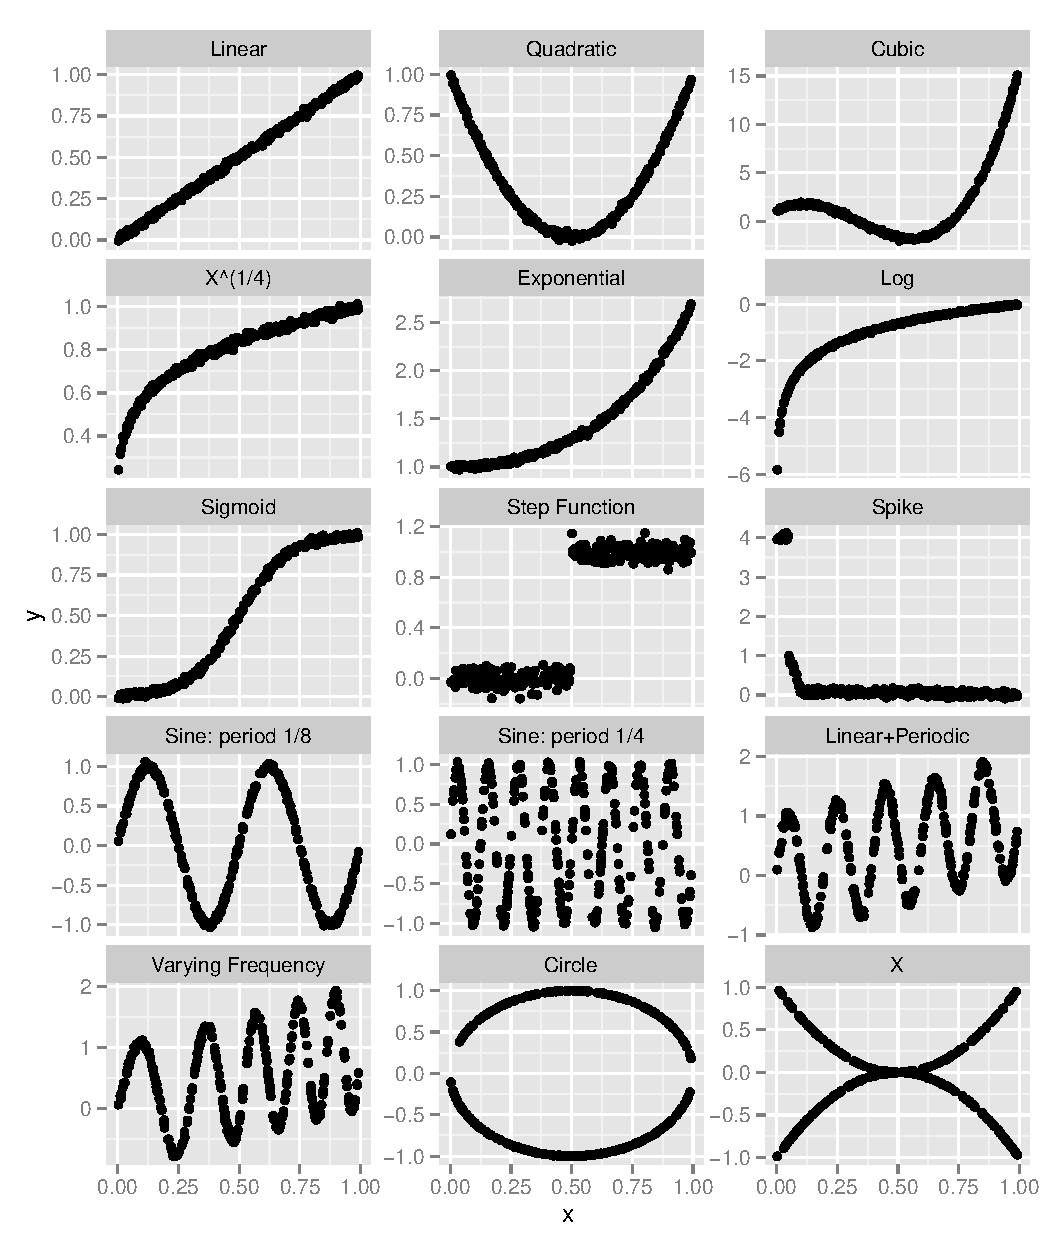
\includegraphics[width=\textwidth]{FunctionFormsNoNoise.pdf}
\caption{Scatter plots showing the fifteen different functional forms being evaluated. } 
\label{F:FunctionForms}
\end{centering}
\end{figure}


\section{Power versus Noise}
In order for an association measure to be practically useful in association analysis it should have reasonable statistical power for noisy data. Ideally it should also be equitable, i.e. it should score equally different types of relationships with equal amounts of noise added. This simulation explored how statistical power varied for the different functional forms for different amounts of Normally distributed noise. A sample size of 320 was used to represent a moderately size biological dataset. (Figure \ref{F:FunctionFormsNoise} in Appendix A shows each functional form following the addition of noise.) 

Data was generated using two  distributions, \textit{Uniform(0.1)} and \textit{Beta(2,5)}, so for a  r.v. $X$, $X \in \{0,1\}$. Random noise was generated from a $N(0,1)$ distribution and then scaled by a given noise level (0.1 to 3). The following algorithm was used in the simulation to assess if two r.v.'s $X$ and $Y$ were dependent:

\begin{enumerate}
\item For each functional form, $f$, and noise level, $l$:
\item Generate independent r.v.'s $X,Y$ and $Z$: $X$ and $Z$ from the given distribution (so $X \in \{0,1\}, Z \in \{0,1\}$) and an independent r.v. $Y=f(Z) + l \times \epsilon$, where $\epsilon \sim N(0,1)$.
\item Measure the association between $X$ and $Y$ using $A$, $dcor$, $MIC$, $\rho_{pearson}^2$ and $\rho_{spearman}^2$
\item Generate dependent r.v.'s $X$ and $Y$: $X$ from the given distribution and a dependent r.v. $Y=f(X) + l \times \epsilon$, where $\epsilon \sim N(0,1)$. 
\item Measure the association between $X$ and $Y$ using $A$, $dcor$, $MIC$, $\rho_{pearson}^2$ and $\rho_{spearman}^2$
\item Estimate the power as the number of times the association score for the dependent data exceeds the $95^{th}$ percentile of the corresponding score for the independent data.
\item Repeat $500$ times.
\end{enumerate}

The complete $R$ code, based on that of \citet{Tibshirani2011}, is given in Appendix A. The results in Figure \ref{F:powerNU} suggest that all measures are sensitive to the level of noise and that none of the measures has greater power for all of the functional forms simulated. In particular $A$ appears to have low power for the fourth root, step, exponential, sigmoid and linear cases. It also has lower power than $dcor$ in the cubic cases. Both $A$ and $MIC$ generally outperform $dcor$ for periodic functions most notably for the high frequency sine wave. Interestingly, $A$ has the highest power in detecting the circle and `X' shapes.

Simulation results from the skewed distribution were broadly similar to that shown in Figure \ref{F:powerNU} are given in Appendix A.2 (Figure \ref{F:powerNB}). For most functional forms there was a decrease in power, most notably for the step function which showed a reduction in power for all association measures. Both $A$ and $MIC$ also had lower power than Pearson correlation in the quadratic and cubic cases.

\begin{figure}[H]
\begin{centering}
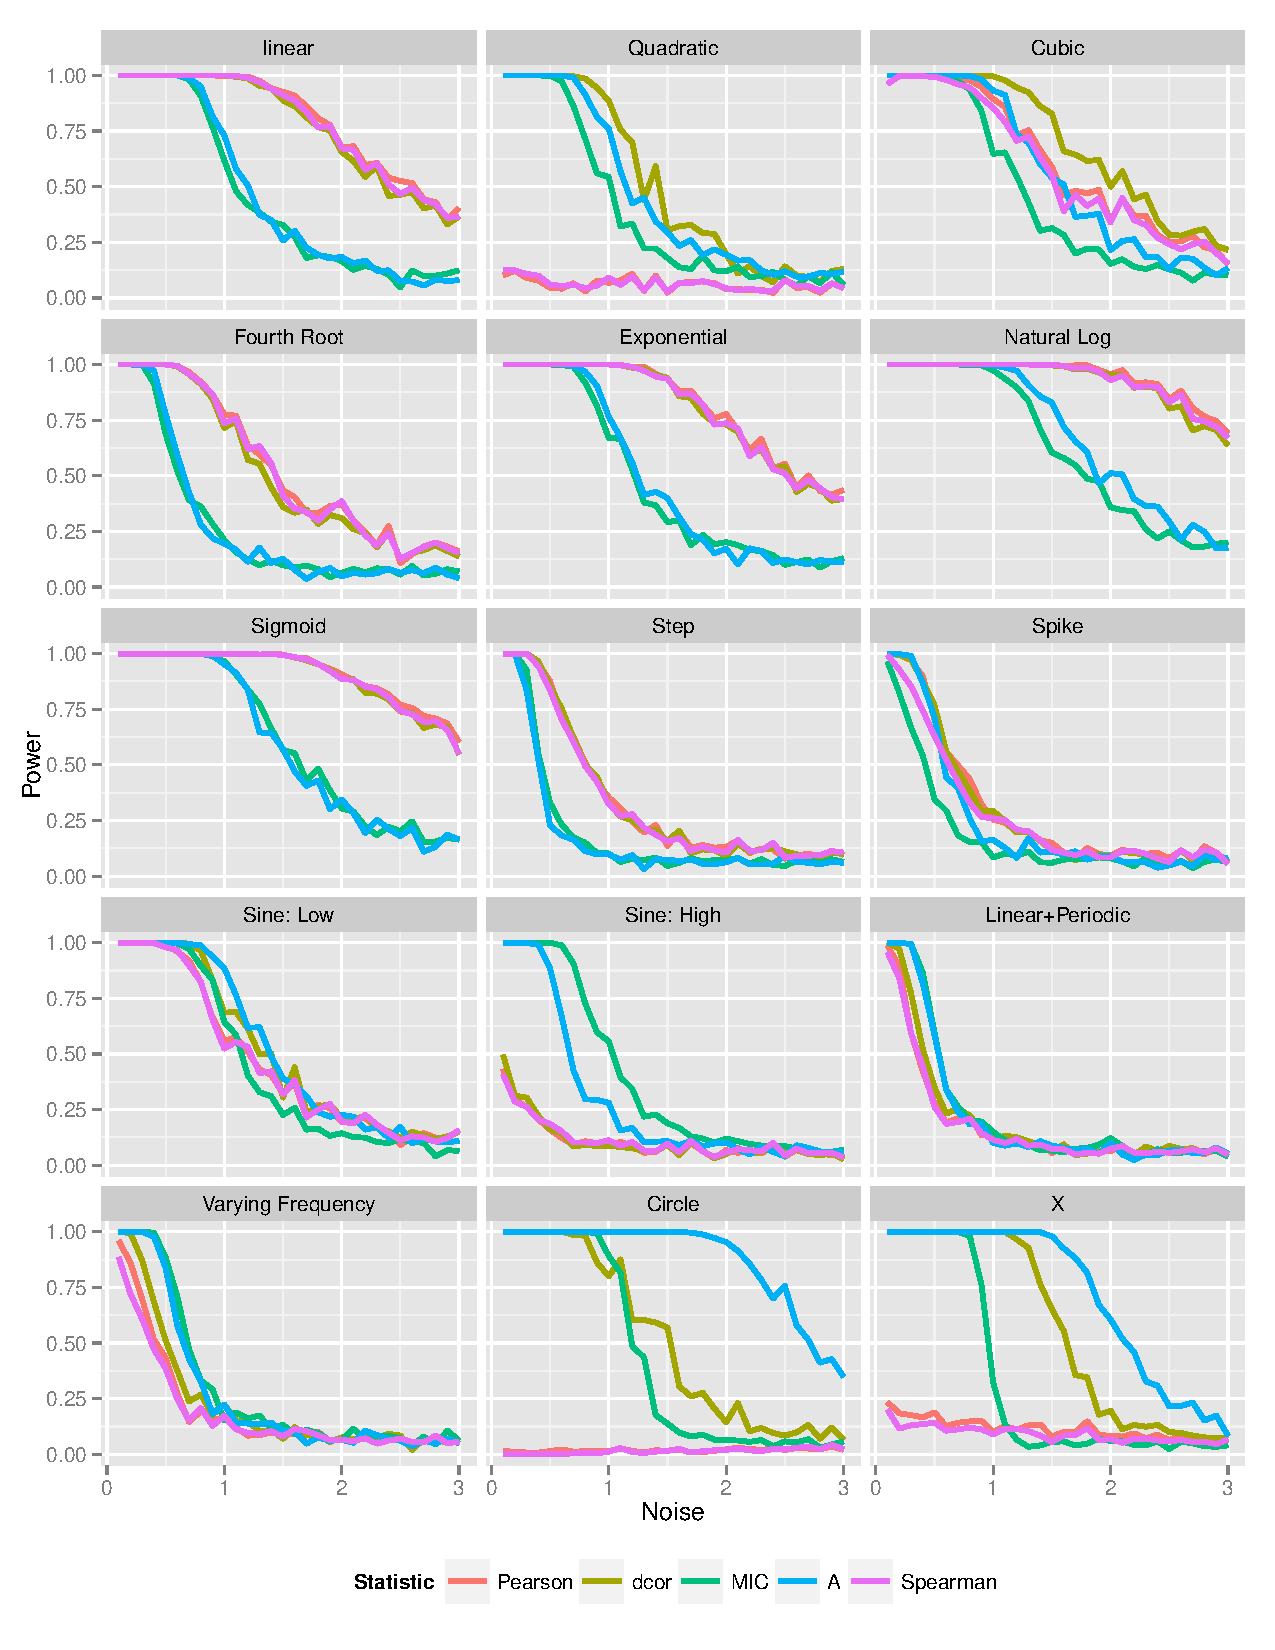
\includegraphics[width=\textwidth]{powerNoiseUN.pdf}
\caption{Scatter plots showing the power of each measure of association vs. noise for each functional form based on 320 observations from a $Uniform(0,1)$ distribution.} 
\label{F:powerNU}
\end{centering}
\end{figure}

\section{Power versus Sample Size}
Typically for biological datasets the sample size, $n$, is relatively small (in the case of the lupus dataset $n = 420$), while $n > 1000$ would generally considered a large dataset. Hence to be of practical use an association measure should be sufficiently powerful at detecting associations on small datasets. This was the objective of this simulation.  

An adapted version of algorithm given in the previous section was used to explore how power varies with sample size in the presence of moderate noise:

\begin{enumerate}
\item For each functional form, $f$, and sample size, $n\in$ \{10, 20, 30, 40 ,50, 75, 100, 125, 150, 200, 250, 300, 350, 400, 500, 750, 1000\}:
\item Generate independent r.v.'s $X,Y$ and $Z$: $X$ and $Z$ from the given distribution (so $X \in \{0,1\}, Z \in \{0,1\}$) and an independent r.v. $Y=f(Z) + l \times \epsilon$, where $l=1$ and $\epsilon \sim N(0,1)$
\item  Measure the association between $X$ and $Y$ using $A$, $dcor$, $MIC$, $\rho_{pearson}^2$ and $\rho_{spearman}^2$
\item Generate dependent r.v.'s $X$ and $Y$: $X$ from the given distribution and a dependent r.v. $Y=f(X) + l \times \epsilon$, where $l=1$ and $\epsilon \sim N(0,1)$. 
\item  Measure the association between $X$ and $Y$ using $A$, $dcor$, $MIC$, $\rho_{pearson}^2$ and $\rho_{spearman}^2$
\item Estimate the power as the number of times the association score for the dependent data exceeds the $95^{th}$ percentile of the corresponding score for the independent data.
\item Repeat $500$ times.
\end{enumerate}

Again the algorithm was run with a \textit{Uniform(0,1)} distribution and then with a \textit{Beta(2,5)} distribution to see if a skewed source distribution affected the results. The results for the \textit{Uniform} case are given in Figure \ref{F:powerSizeUN10}. The results show that $A$, $MIC$ and $dcor$ only converged in certain cases but that $dcor$ converged more quickly (i.e. is more powerful on smaller sample sizes) in the linear, quadratic, cubic and exponential cases. The power of $dcor$ was again noticeably low in the high frequency sine case. No measures converged for the step, spike, linear+periodic or varying frequency functions function. $A$ and $MIC$ both failed to converge for $X^{\frac{1}{4}}$.

\begin{figure}[H]
\begin{center}
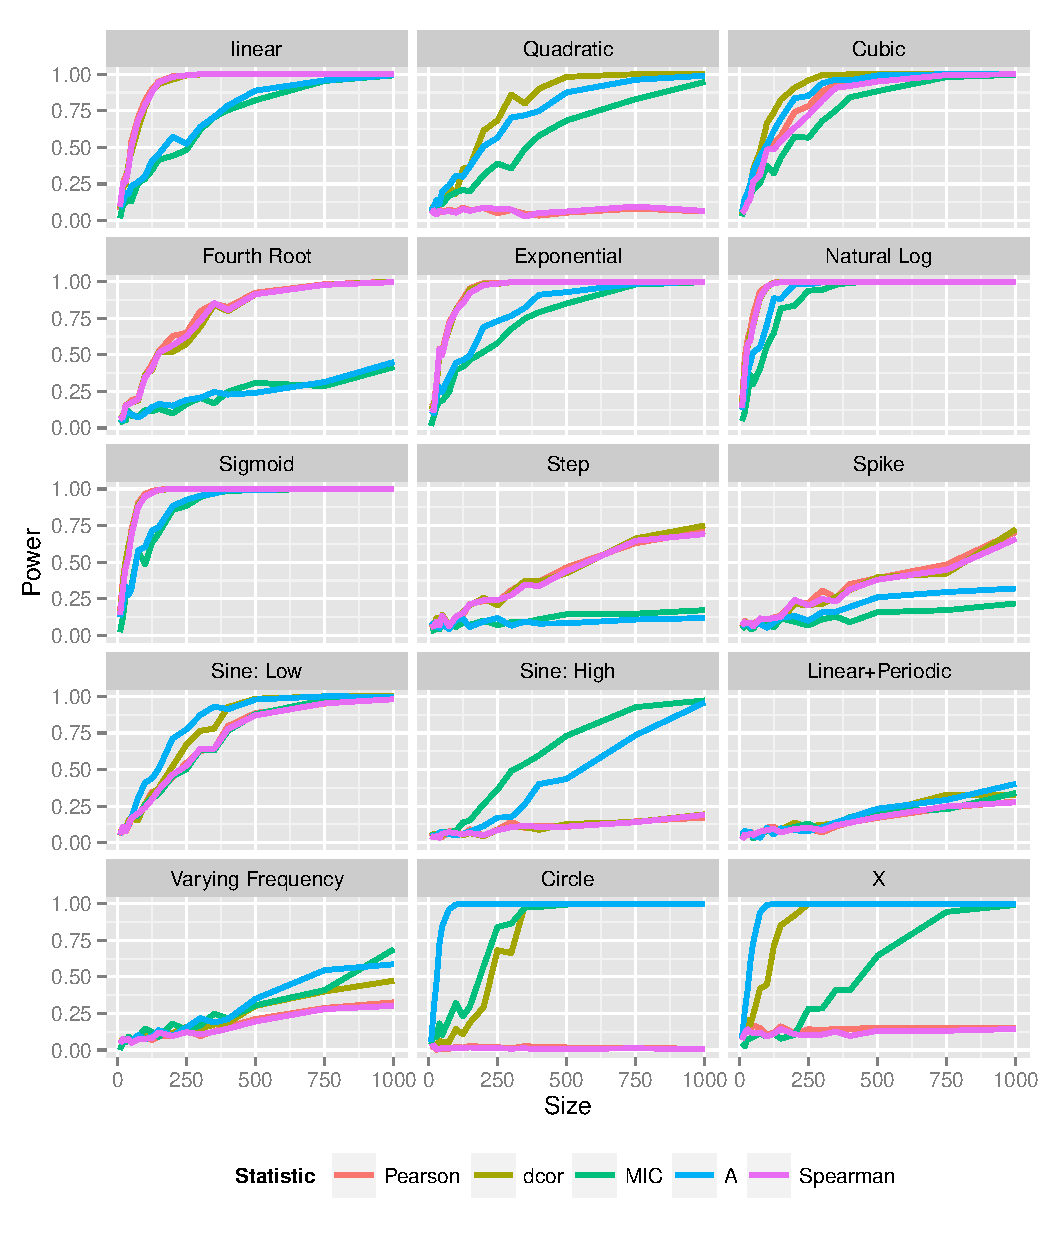
\includegraphics[width=\textwidth]{powerSizeUN10.pdf}
\caption{Scatter plots showing the power of each measure of association vs. sample size using a $Uniform(0,1)$ distribution.} 
\label{F:powerSizeUN10}
\end{center}
\end{figure}

In the case of the skewed distribution, the performance of all measures generally declined, particularly for $A$ and $MIC$ in the quadratic and cubic cases. The power of $A$, $MIC$ and $dcor$ also reduced for the exponential function. The results are shown in Figure \ref{F:powerSB} in Appendix A.

Simulations were also run using the maximum level of noise and using a skewed distribution. The results are shown in Figure \ref{F:powerSizeBN30} in Appendix A.2 and show that none of the association measures were powerful at detecting dependence on very noisy relationships even when the sample size was large ($n=1000$).

\section{Discussion}
The simulation studies focused on how the power of the different measures of association perform in the presence of noise and with different sample sizes. This is of particular relevance to biological datasets which can contain a large amount of technical variability which is not of interest and typically have small sample sizes but many dimensions. 

Unsurprisingly the simulations showed that in general power decreases in the presence of increasing noise while power increases with increased sample size even in the presence of noise. Of greater importance is that the analysis suggested that $A$ suffers from some of the same power deficiencies as $MIC$ for certain important cases such as linear and cubic but both surpass $dcor$ where high frequency periodic variation exists. This appears to confirm the reservations regarding the equitability heuristic expressed by \citet{Kinney19082014} and \citet{Tibshirani2011}. The size simulations questions the practical usefulness of the generality heuristic.

No one measure exceeded all of the others in all of the cases, however on balance the simulation study suggests that $dcor$ should perform better than either $MIC$ or $A$ on the basis of capacity to handle noise and deal with small sample sizes. From a practical perspective if the form of a relationships are unknown then $dcor$ would appear to be the best choice of association measure, possibly in conjunction with Pearson Correlation (to assess non-linearity) and either $A$ or $MIC$ if periodic effects are suspected or known a priori.

There are many other simulation based analyses that could be performed. The noise and size studies both held either size or noise constant, an obvious extension would be to allow both noise and sample size to vary simultaneously to get a more complete power profile.  Further extensions would be to expand the range of functional forms and source distributions and to include three way and partial associations where possible. Additionally it would be of interest to explore  relative performance of $HHG$ \cite{HHG} which has been identified as being of potential use for exploratory association mining. 

\chapter{Exploratory Data Analysis} 
This section documents exploratory analysis of the training dataset. The objective of this analysis was to explore a subset of gene expression data relevant to lupus in order to search for genes and gene associations of potential interest. A range of supervised and unsupervised techniques were employed. Most of the exploratory analysis analysed lupus patients and controls separately in order to focus on non-linear gene relationships that differ between the two classes. A drawback of this approach is that the sample size for controls is relatively small at 53 observations and hence potentially subject to the power deficiencies identified during simulation.

\section{Data} 

\subsection*{Description}
Two Affymetrix microarray datasets were provided as follows:

\begin{enumerate}
\item A training dataset consisting 420 observations (53 controls, 367 lupus patients) of 94 gene expressions deemed to be of biological interest.
\item A test dataset containing 1024 observations of 54,675 probes. 628 of the observations could not be identified as either a lupus patient or a control so these were excluded from the analysis. Hence in the reduced dataset there were 29 controls and 367 lupus patients.
\end{enumerate}

Both sets of gene expression data had been standardised using an algorithm known as GCRMA \cite{GCRMA} which applies a statistical model to correct background expression levels which arise as an artefact of the microarray measurement process. The resultant data are unitless and on a $log_2$ scale meaning that values don't have any direct interpretation in an absolute sense, but only in a relative sense in that a subject with a value of 3 for a gene will have an expression twice as high for that gene as a subject with a value of 2. No demographic information about samples was provided. No replicates existed hence it was not possible to assess how much technical variability existed.

The data as given only contained the Affymetrix probe IDs. In order to provide additional context information the probe IDs were annotated using the Affymetrix Human Genome Focus Array data in the $hgfocus.db$ \cite{hgfocus.db} Bioconductor R package in order to map the probes to associated genes and assign a genetic locus (chromosome and chromosome location). Some probes did not have any associated annotations so supplemental hand annotations were made using the GeneAnnot\cite{GeneAnnot} search engine. This was of secondary interest but provided additional context information for discussing observed variability, for example to show that co-expressed genes may be genetically distant or that individual probes may map to the same gene. Table \ref{T:Data} describes the data in more detail. 

\begin{table}[ht]
\begin{centering}
\begin{tabular}{llllll}
  \hline
 Variable & Type & Description \\ 
  \hline
Diseased & Factor & A two level categorical variable indicating whether or not \\ 
  & & a patient has lupus.\\
&& Levels: Lupus, Control \\
Sample ID & String & A string which uniquely identifies a human blood sample. \\
 & & Samples were drawn from multiple sources with the prefix \\
&& of the Sample ID identifying a distinct source. \\ 
Source & Factor & A categorical variable identifying subgroups of samples \\
 & & based on the sample source. \\ 
&& Levels: C, L1, L2, L3, L4, L5 \\
Probe ID & String & Uniquely identifies an Affymetrix DNA probe used to \\
  && identify a gene. A probe is associated with a single gene. \\
Expression  & Continuous &  The level of gene expression for a particular \\
&& probe in a sample.\\ 
Chromosome & Factor &  The chromosome which the probe binds to. \\
&& Levels: 1 to 22, X\\
Chromosome & Integer &  The start binding location on the chromosome \\
Location && measured in base pairs. \\
Gene & String &  The gene associated with a probe. A gene can be \\
&& associated with many probes. \\
Probe Number & Integer & A locally unique number identifying a probe within a \\ 
&&single dataset. Used for convenience to simplify analysis.  \\
   \hline
\end{tabular}
\caption{Descriptions of the variables analysed.} 
\label{T:Data}
\end{centering}
\end{table}

\subsection*{Visualisation}
The density plots in Figure \ref{F:Density} show the distributions of each probe separately for both controls and lupus patients. Following the standardisation procedure the expression of each gene is zero centred. The plots suggest that some gene expressions have a skewed distribution and this is clearly shown in Figure \ref{F:Box}.

\begin{figure}[H]
\begin{centering}
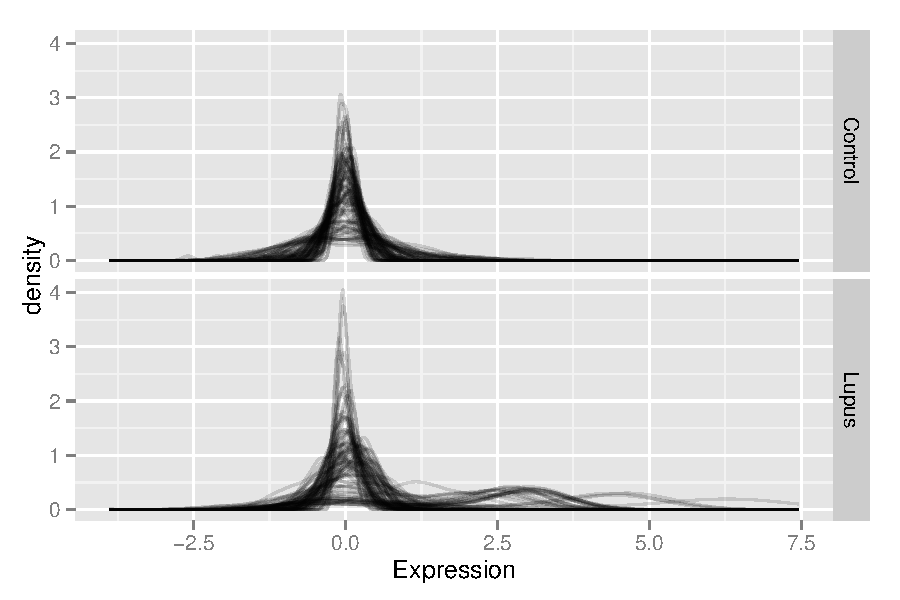
\includegraphics[width=\textwidth]{densities.pdf}
\caption{Densities of gene expression for lupus patients and controls suggesting higher expression levels and greater variability in lupus patients than controls.} 
\label{F:Density}
\end{centering}
\end{figure}

The boxplots in Figure \ref{F:Box} suggest differences in gene expression levels between lupus patients and \gls{Control}s. \gls{Lupus} patients appear to have higher expression levels and greater variability for many of the genes. Both groups have potential outliers for many of the genes. Figure \ref{F:Box} suggests that genetically distant genes are co-expressed in lupus patients.

\begin{figure}[H]
\begin{centering}
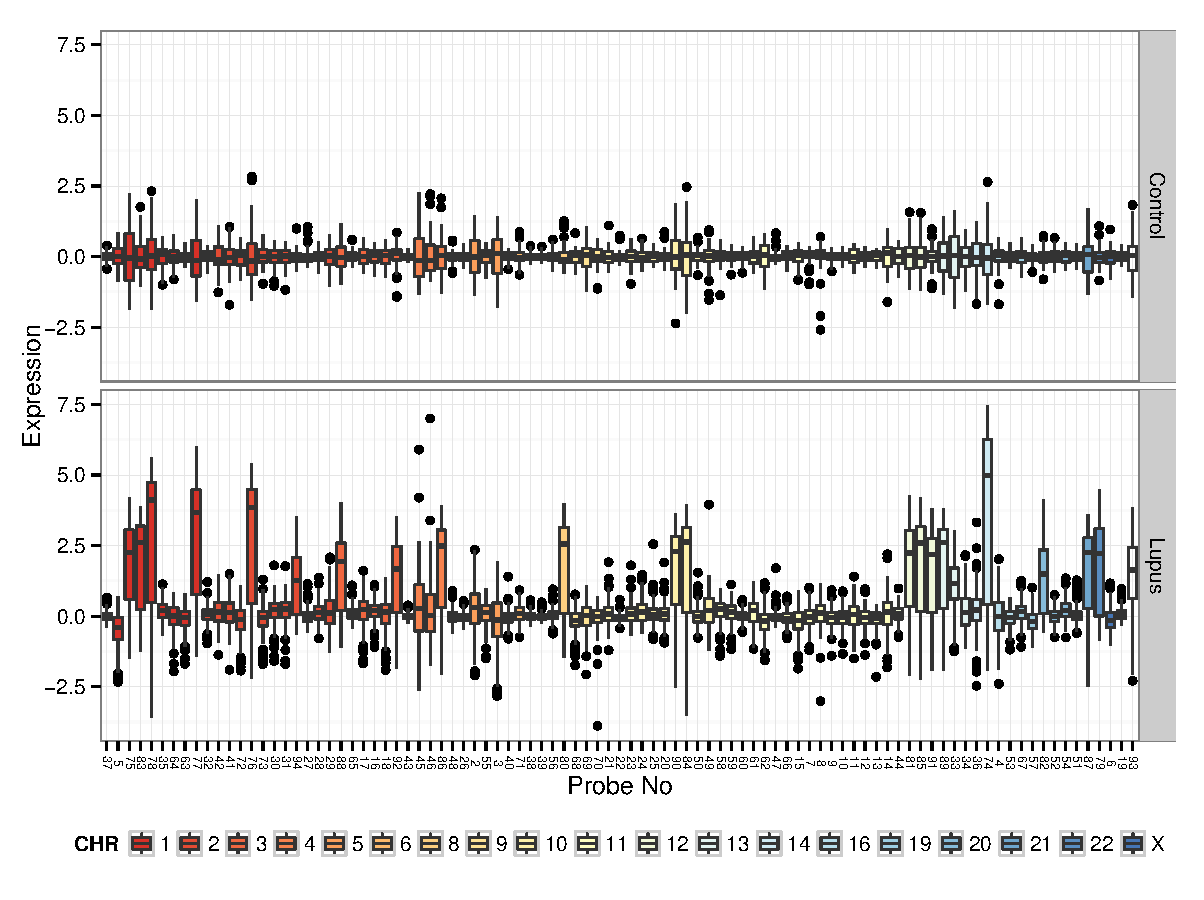
\includegraphics[width=\textwidth]{boxAll.pdf}
\caption{Boxplots of gene expression for controls and lupus patients suggesting higher expression levels and greater variability in lupus patients than controls. The probes are coloured by chromosome and ordered by chromosome and chromosome location.} 
\label{F:Box}
\end{centering}
\end{figure}

%Heatmaps are a useful exploratory tool for visualising a large dataset in two dimensions. 
The heatmap in Figure \ref{F:heat} gives a visualisation of the full training dataset (94 genes, 420 samples).  The colour in each cell represents the gene expression level of each gene for each sample. Blue represents high gene expression while white represents low expression. It clearly shows the apparent elevated elevated expression levels of certain genes in lupus patients. The heatmap was created by clustering the genes and samples separately to try to give structure to the data. Clustering methods aim to separate the data into a set of distinguishable groups based on some distance metric. %Clustering was used to try to identify groups of related genes based on the non-linear part of association which was converted into a dissimilarity metric by subtracting one. 
In this case the distance metric used was $1 - A$ in order try to capture both linear and non-linear relationships. The aim was to try to identify if genes cluster into distinct groups that differ between lupus patients and controls. The dendrogram for the genes shows that genes on some chromosomes seem to have similar expression levels while the block of highly expressed genes to the right are located on different chromosomes. Clustering did not clearly separate all lupus patients from controls but suggests that differences within lupus patients exist.

\begin{figure}[H]
\begin{center}
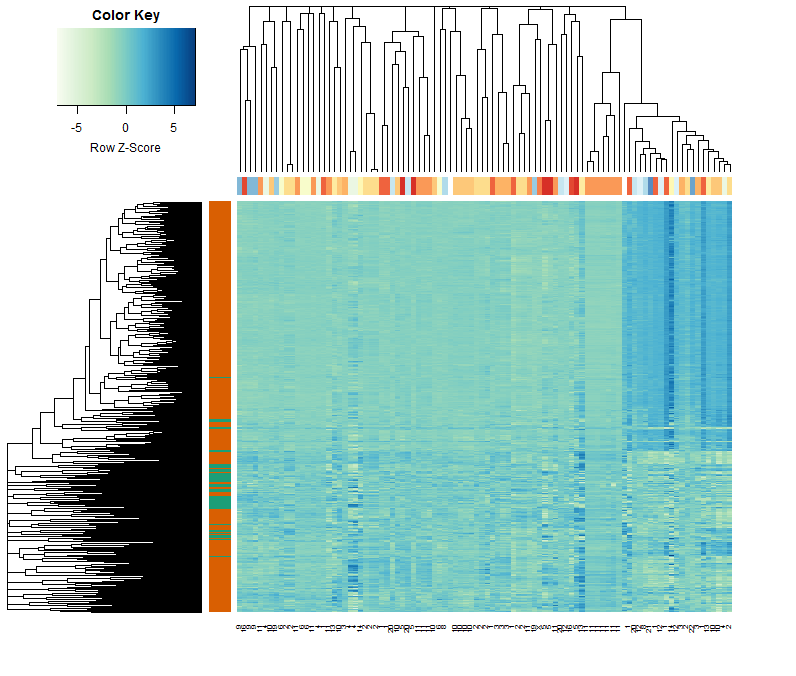
\includegraphics[width=\textwidth]{heat3.png}
\caption{Heatmap of gene expression of probes of biological interest. Clustering of probes and samples used $1-A$ as the distance metric. The band on the rows uses green for controls and orange for lupus patients. The column band and labels represents chromosome.} 
\label{F:heat}
\end{center}
\end{figure}

\subsubsection{Association}
The number of dimensions make direct visualisation of pairwise gene relationships using scatterplots difficult. An alternative approach is to use a form of heatmap known as correlation plots (corrplots) to  give a high level view of the pairwise correlations. They represent this graphically using a colour map where each square shows the correlation score between two variables. Colour is used to show the direction of correlation with positive correlation shown as blue, negative correlation shown as red and no correlation is shown as white. The strength of the colour indicates the strength of the correlation. 

The correlation plots in Figure \ref{F:Corr} show correlation plots for controls (left) and lupus patients (right) using Pearson correlation (top panel), $A$ (middle panel) and $dcor$ (bottom panel). The top panel shows that both lupus patients and controls have strong negative and positive Pearson correlations for different genes. Other genes appear uncorrelated. The training set appears to showing much stronger correlations for lupus patients than controls. Association plots based on $A$ confirm the strong association between some genes but also appear to have lower association scores for many genes as compared with Pearson correlation. A possible explanation for this is the lack of power for $A$ in the linear case when sample sizes are small (53 in the case of controls). The $A$ based corrplot does not suggest any strong, possibly non-linear, associations that were not detected by Pearson correlation. The $dcor$ based correlation plot of controls (bottom left) shows a higher pairwise association than either Pearson correlation or $A$. 

Corrplots allow a direct high level view of associations however the density of the information in the plots means that their usefulness is limited.  Dimension reduction offers other efficient alternatives and is explored in the next section. 

(Note: the $A$ and $dcor$ based corrplots were sign adjusted to allow easier comparison with the Pearson corrplots. This was performed by multiplying the association score by the sign of the corresponding Pearson correlation.) 

\begin{figure}[H]
\begin{centering}
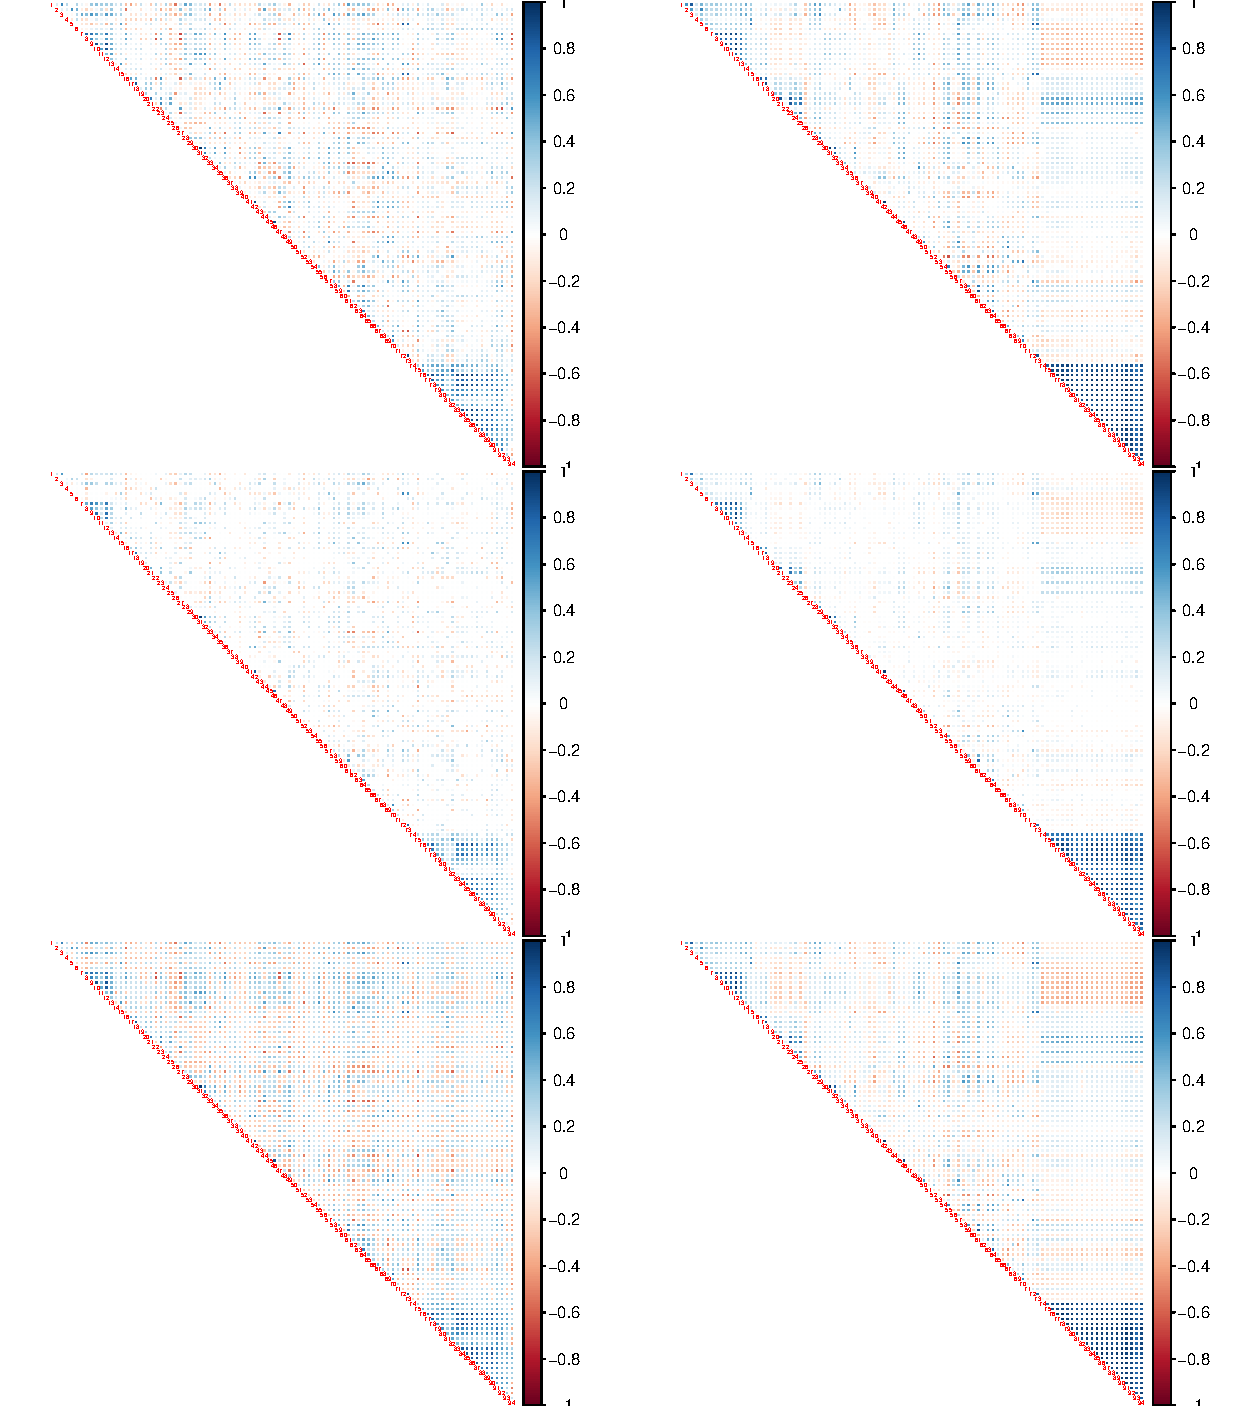
\includegraphics[width=\textwidth]{corrplot3.pdf}
\caption{Corrplots visualising association matrices of all 94 probes. The probes are ordered by probe number. The left side is controls, the right side is lupus patients. The top panel uses Pearson correlation. The middle panel uses correlation sign adjusted $A$ score. The bottom panel uses correlation sign adjusted $dcor$.} 
 \label{F:Corr}
\end{centering}
\end{figure}

\section{Dimension Reduction}
A variety of dimension reduction techniques were applied to the training dataset in order to explore structure in both the variables and the samples. Both linear and non-linear techniques were used as a possible way of highlighting any potential non-linear relationships of interest.

\subsection*{Principal Component Analysis}
\gls{PCA} was performed on the data in order to assess how effective linear based dimension reduction is on the training dataset. Due to the variability of the data, PCA based on the correlation matrix was used. The corrplots in Figure \ref{F:Corr} showed that many variables were highly correlated suggesting that PCA would be an appropriate choice for reducing the dimensions for exploratory analysis. A screeplot (not included) suggested that about 80\% of the variation is explained by the first two principal components but the amount of variation explained by subsequent principal components tailed off slowly. The scatter plot in Figure \ref{F:PCA} shows that controls and lupus patients are not clearly distinguished by the first two PCs. The loadings in Figure \ref{F:PCALoadings} suggest that much of PC1 is dominated by the genes with strong Pearson correlations indicated in the correlation plots in Figure \ref{F:Corr} (Probe No.'s 74 to 94). The controls are clearly associated with positive values of PC1 but so are many lupus patients. %This suggests that PCA has limited use for this dataset.

\begin{figure}[H]
\begin{centering}
\includegraphics[width=\textwidth]{pc12.pdf} 
\caption{The first two principal components.} 
 \label{F:PCA}
\end{centering}
\end{figure}

\begin{figure}[H]
\begin{centering}
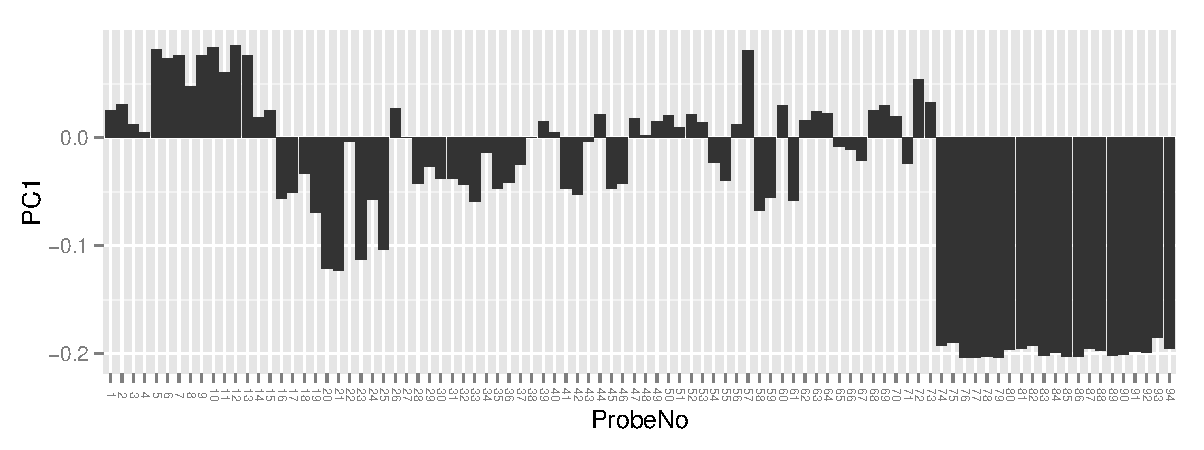
\includegraphics[width=\textwidth]{loadings.pdf} 
\caption{PC1 loadings.} 
 \label{F:PCALoadings}
\end{centering}
\end{figure}

\subsection*{Linear Discriminant Analysis}
Linear Discriminant Analysis (\gls{LDA}) is a form of dimension reduction that, for $k$ given classes attempts to find $k-1$ projected variables called linear discriminants (also called crimcoords). Thus, it attempts to find a reduced dimensional space that maximises inter class distance. It is a linear based technique with the first linear discriminant corresponding to Fisher's linear discriminant function. The remaining crimcoords are often interpreted in a similar way to Principal Components but differ in that they are not orthogonal but by convention are often plotted as such. 

\begin{figure}[H]
\begin{centering}
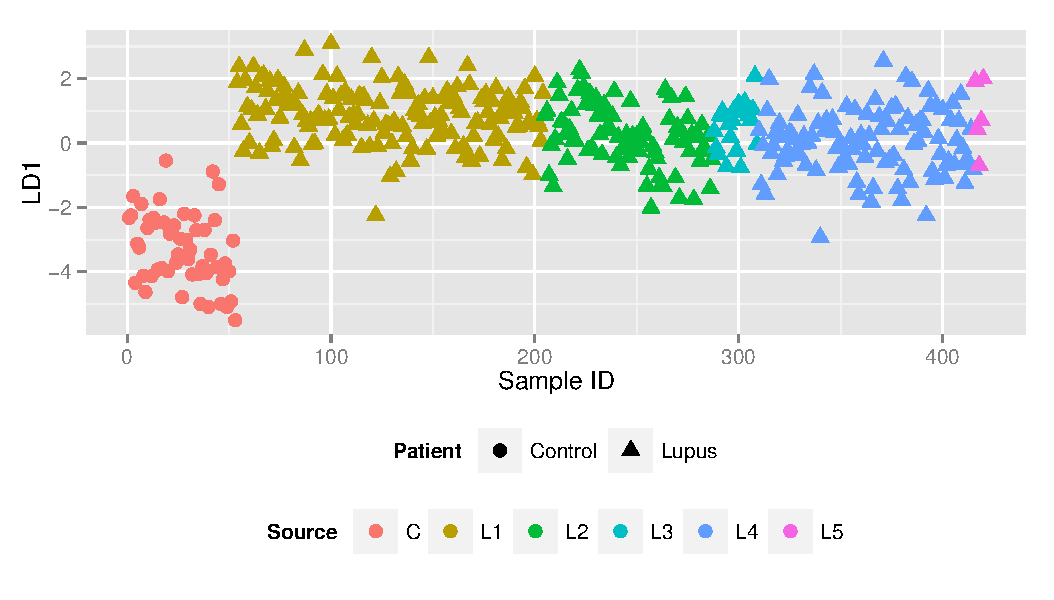
\includegraphics[width=\textwidth]{lda} 
\caption{The first linear discriminant of lupus vs. controls plotted against index.} 
 \label{F:LDA}
\end{centering}
\end{figure}

\begin{figure}[H]
\begin{centering}
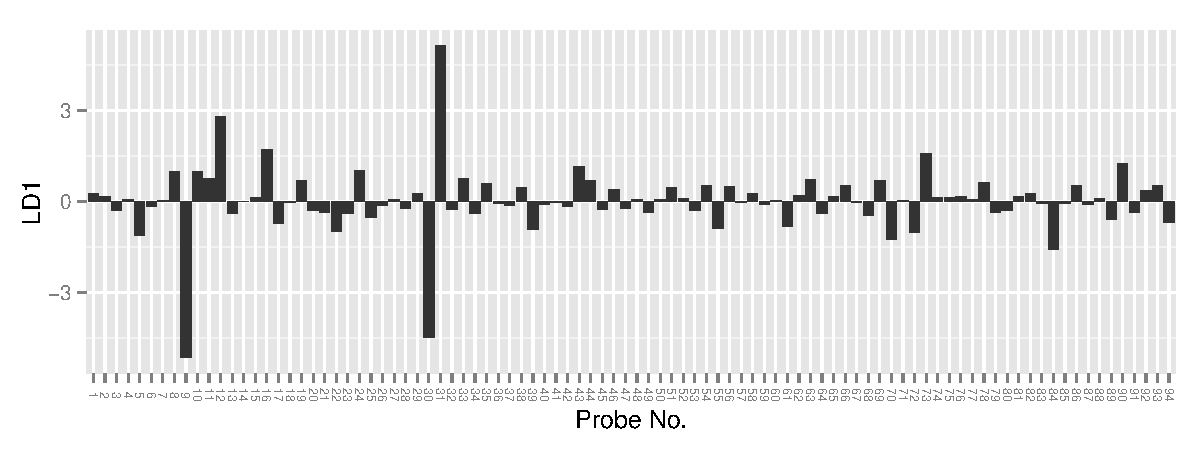
\includegraphics[width=\textwidth]{ldaScalings} 
\caption{The scalings from the first linear discriminant of lupus vs. controls.} 
 \label{F:LDAScalings}
\end{centering}
\end{figure}


Figure \ref{F:LDA} shows a crimcoord plot of the training dataset using the disease status as the response variable. It suggests that linear discrimination based on gene expression difference between lupus patients and controls is reasonably successful which again suggests the importance of linear relationships in this dataset. In general the two groups are well separated however overlaps exist. The scalings in Figure \ref{F:LDAScalings} suggest that four probes in particular (Probe No's 9, 30 for controls and Probe No 12 an 31 for lupus patients) contribute a large amount to discriminating patients and controls. 

LDA was also performed using Source as the response variable and the results are shown in Figure \ref{F:LDAType}. The results are interesting in that some lupus sources appear to be well separated based on a linear combination of genes. The first crimcoord appears to separate lupus source L1 and L2 from the controls and L4. The second crimcoord clearly separates lupus source L3 from the rest. While the fourth crimcoord separate lupus source L5 from the rest. The associated scalings (not shown) suggested that Probe No 9, 30, 31 and 32 have most weight. Probe No 32 did not appear to have much discriminatory power in separating lupus patients from controls.

\begin{figure}[H]
\begin{centering}
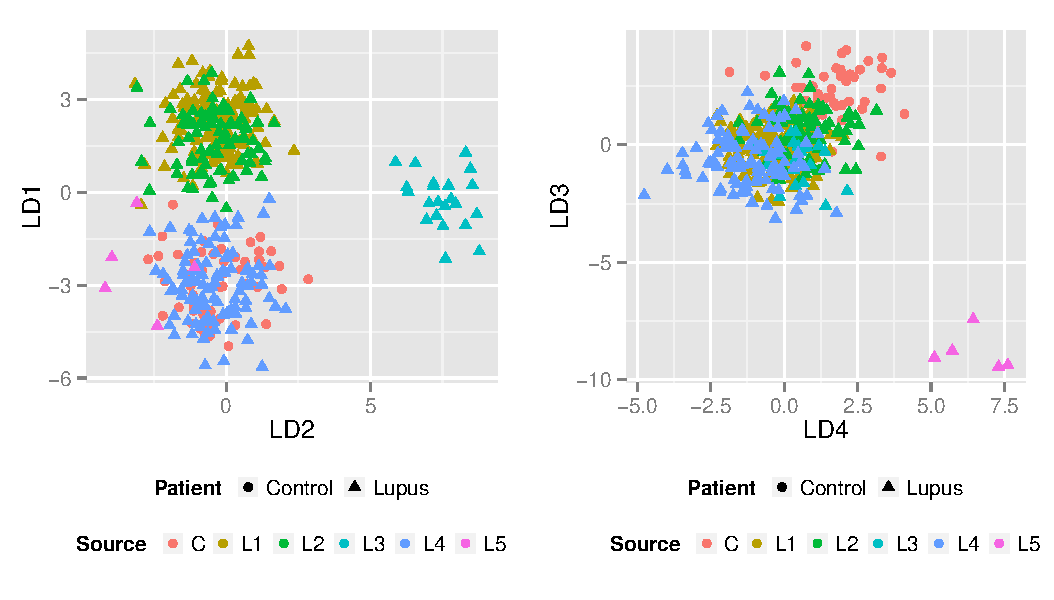
\includegraphics[width=\textwidth]{ldaType.pdf}
\caption{LDA based discrimination of sample sources.} 
 \label{F:LDAType}
\end{centering}
\end{figure}

\subsection*{Multidimensional Scaling}
Multidimensional scaling (MDS) is another form of dimension reduction that is useful for exploratory data analysis. There are a number of different variants of \gls{MDS}. In this case a technique called Sammon scaling was used which creates a non-linear low dimensional projection of the data based on a given distance metric. Sammon scaling has the advantage of being able to preserve small distances in the reduced dimensional space. 

In contrast to the previous analyses, MDS is used to project the genes into two dimensions. In order to try to assess if differences  between $R^2$, $A$ and $dcor$ existed these were all used as distance metrics in the MDS plots in Figure \ref{F:MDS}. Scree plots (not included) suggested that the first two components captured most of information but that 3 or 4 dimensions best describes the data, hence some distortion is present. 

Figure \ref{F:MDS} shows pronounced differences between controls and lupus patients. The scaling plots for the lupus patients show a tight cluster of genes (Probe No 74 to 94) that are reasonably well separated and consistent (ignoring reflection) between the three methods. These genes showed very high Pearson correlation and suggest that the strongest pairwise gene associations can be described well using linear methods. No other obvious gene clusters are visible in the lupus MDS plots although individual gene distances vary considerably between the different methods. 


\begin{figure}[H]
\begin{center}
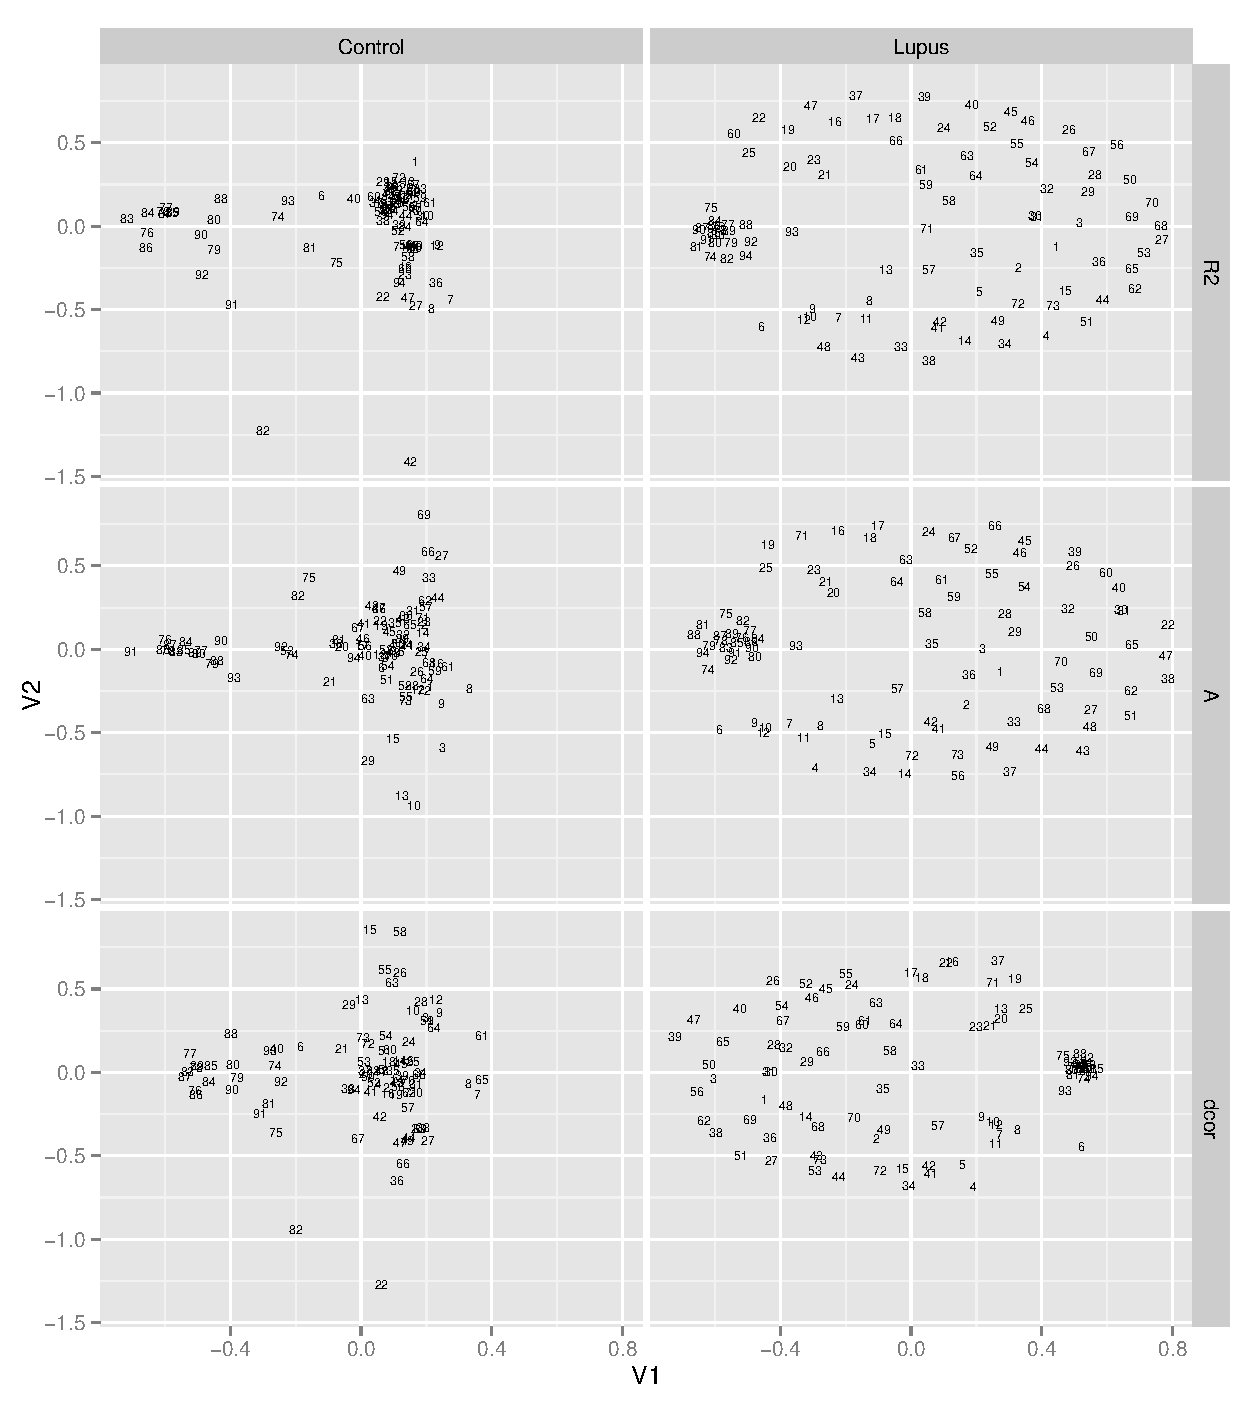
\includegraphics[width=\textwidth]{MDS.pdf}
\caption{2D MDS of the probes of the training data. The top plots used $1-R^2$ as a distance measure, the middle plots used $1 -  A$,  while the lower plost used $1 - dcor$.}
\label{F:MDS}
\end{center}
\end{figure}

\subsection*{Flexible Discriminant Analysis}
Flexible Discriminant Analysis (\gls{FDA}) is a classification technique related to \gls{LDA}. While LDA uses hyperplanes to form decision boundaries, FDA can fit curved surfaces and hence is better suited to exploring non-linear relationships. FDA works by using regression in the classification process using a procedure called optimal scoring to create a derived response variable \cite{earth}. An advantage of this approach is that it can accommodate a range of different regression techniques. In this case, the FDA model was built using Multiple Adaptive Regression Splines (\gls{MARS}) so the FDA discriminant planes are based on the underlying MARS model. Another useful feature of FDA/MARS is that it can treat predictor variables both singly or allow higher order interactions. MARS uses an iterative procedure of regression fitting to build a model from the data. Forward and backward steps, similar to stepwise regression, along with generalized cross validation are used to try to mitigate over-fitting the model \cite{EOSL} and also to rank variable importance \cite{earth}. In contrast to some other data mining techniques such as neural networks the model results are easily interpretable in terms of the input variables and is therefore particularly suited to exploratory analysis. The R packages $mda$ \cite{mda} and $earth$ \cite{earth} were used.

An important consideration in data mining is explanatory power, which can be assessed through the misclassification rate. The results of allowing differing levels of variable interaction are shown Table \ref{T:MARSFIT}.

\begin{table}[h]
\centering
\begin{tabular}{lll}
  \hline
Variable Interaction & Misclassification Rate \\ 
  \hline
None &  0.028 \\ 
Two-way &  0.019 \\ 
Three-way & 0.002 \\
   \hline
\end{tabular}
\caption{Misclassification rate of different MARS based FDA models.} 
\label{T:MARSFIT}
\end{table}

While the misclassification rate drops to almost zero by allowing two or three way interactions the underlying models are probably over fit to the data. Despite this they provide a means to look at potential interactions of interest. For pairwise relationships the FDA model showed good performance with a training misclassification error of 0.02 (rounded to 2 d.p.). The confusion matrix is  shown in Table \ref{T:confusion1}.  The underlying MARS model had an $R^2$ value of 0.80 (to 2 d.p.). Partial dependency plots showing the relationship of the most important predictor (or predictor pairs) to the FDA discriminant are shown in Figure \ref{F:MARS}. 

\begin{table}[h]
\centering
\begin{tabular}{lll}
  \hline
 & Control & Lupus \\ 
  \hline
Control &  47 &  2 \\ 
  Lupus &   6 & 365 \\ 
   \hline
\end{tabular}
\caption{FDA confusion matrix for disease classification based on two-way interactions.} 
\label{T:confusion1}
\end{table}

\begin{figure}[H]
\begin{center}
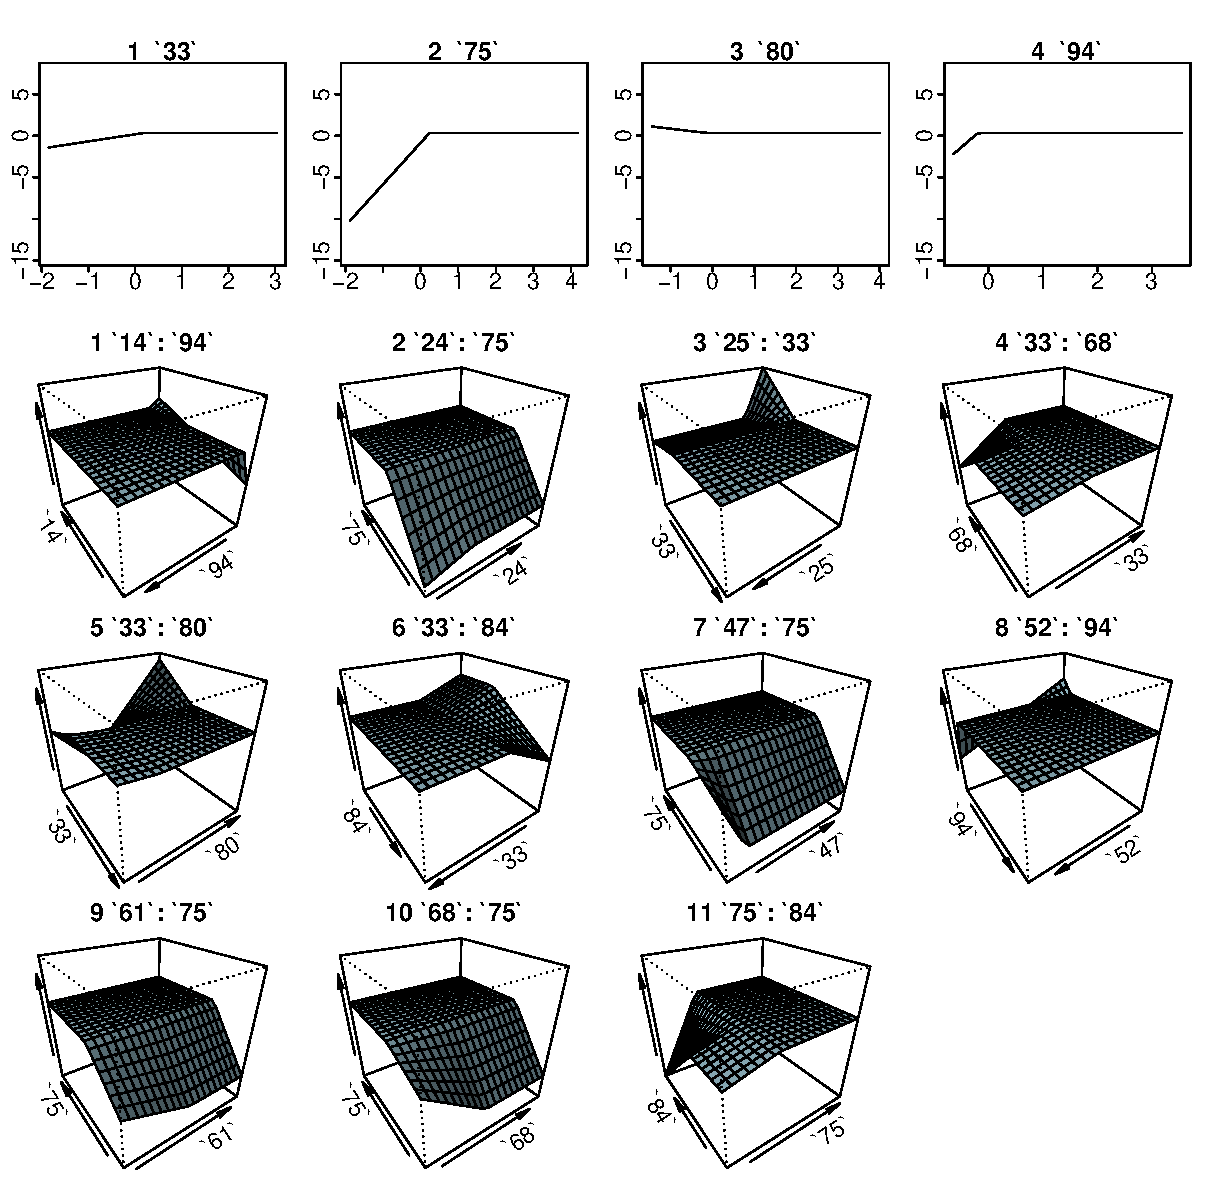
\includegraphics[width=\textwidth]{MARS.pdf}
\caption{Plots of the variables selected by MARS based FDA to classify disease status. The plots are ordered by variable importance. The Y-axis is the FDA discriminant. The subtitle of each plot gives the ranked importance followed by the Probe No(s).}
\label{F:MARS}
\end{center}
\end{figure}

Using \gls{FDA} to classify source had mixed results. The overall misclassification rate was $0.20$ but much of this is due to misclassification of source L1 and L2. When appraising classification results it is important to consider the misclassification cost. Given that both of these sources are lupus patients this misclassification may not be costly in of itself. The misclassification of six controls as source L4 would appear to have a greater cost. The associated confusion matrix is given in Table \ref{T:confusion2}. 

\begin{table}[h]
\centering
\begin{tabular}{rrrrrrr}
  \hline
 & C & L1 & L2 & L3 & L4 & L5 \\ 
  \hline
C &  47 &   1 &   0 &   0 &   6 &   0 \\ 
  L1 &   1 & 132 &  17 &   0 &   5 &   0 \\ 
  L2 &   2 &  16 &  66 &   1 &   5 &   0 \\ 
  L3 &   0 &   0 &   0 &  21 &   0 &   0 \\ 
  L4 &   3 &   2 &   0 &   0 &  90 &   0 \\ 
  L5 &   0 &   0 &   0 &   0 &   0 &   5 \\ 
   \hline
\end{tabular}
\caption{FDA confusion matrix for source classification} 
\label{T:confusion2}
\end{table}

\section{Differential Gene Expression}
Differential gene expression analysis is used to try to understand differences in transcriptional activity between population types which in turn could imply biological differences. In contrast to the other methods in this section it involves formal hypothesis testing. It was used as an exploratory tool in order to:

\begin{enumerate}
\item Validate that the training dataset did in fact contain genes which appear to be associated with lupus.
\item Explore any potential differences between lupus sources.
\item Identify differentially expressed genes to aid in subsequent association analysis.
\end{enumerate}

The primary interest was in differential expression of single genes between lupus patients and controls. Differences between the sample sources were also tested.

A Bioconductor R package called $limma$ \cite{limma} was used to perform the differential expression analysis.  It works by fitting linear models for each gene and can therefore take advantage of the power of linear models to specify complex hypotheses. It also uses a parametric empirical Bayes model to share information between the individual gene models to handle differing levels of variability between genes and between samples and also reduces the influence of outliers. The result is that the global estimate of variability across all genes is combined with the per gene variability to  estimate the variance of  each gene \cite{limma}. While permutation or randomisation tests are often used for this kind of analysis $limma$ has a number of advantages such as the ability to specify contrasts (for example to explore differences in sample sources) and to specify sample correlations e.g. if technical replicates are used.  It is designed to handle small sample sizes and highly dimensional data so is an appropriate choice for the lupus dataset.

The Benjamini Hochberg \cite{FDR} method was used to adjust the $p$-values of the model to try to mitigate the false discovery rate (\gls{FDR}). The main reason for using an adjusted $p$-value is due to what is known as the multiple comparison problem. In a simple $t$-test a widely used convention is to use a critical value of 0.05 for the test. If the test result is a $p$-value of less than 0.05 then this is taken as evidence against the null hypothesis, however there is a 1 in 20 probability that this result could occur by chance alone, i.e. a false positive. (A false positive occurs if the null hypothesis is rejected, when it is in fact true. These are also known as Type I errors.)  In the case of the gene expression data there are 94 hypotheses to test meaning that if the $p$-value is not adjusted we would expect about five false positives to occur. An additional problem is that gene expressions are not independent of one another.

While methods such as Bonferroni corrections can be overly conservative, the FDR addresses the need to use an `adjusted' $p$-value but adopts a less conservative approach and increases the ‘power’ of the test, i.e. increases the probability of identifying significant differences between patients and controls.  FDR adjusted $p$-values are calculated as follows:

\begin{enumerate}

\item Place the $p$-values in ascending order, and label these $p_i$. So $p_1$ will be the smallest $p$-value, and $p_{94}$ the largest $p$-value.
\item Set a significance level to test, e.g. at the 5\% level ($\alpha= 0.05$).
\item Identify $n$, the number of ‘parallel’ tests being conducted, in this case n=94.
\item Starting with the largest $p_i$, identify the first $p_i$ in the sequence for which the following is true: $p_i \le \alpha(i / n)$.
\item Stop at the first $p_i$ that meets this condition, and calculate the `adjusted' $p$-value as $\alpha (i / n)$, using this value of $i$.

\end{enumerate}

A value of $5\%$ was taken to signify differential expression. It is important to note that this is a somewhat arbitrary choice and does not imply biological importance. The interest is in differentially expressed genes where the difference in effect size is large. It is possible to have a significant result as measured by a small $p$-value but which also has a very small effect size and hence is unlikely to be of biological interest. A common convention in microarray studies is to set a minimum for a log fold change value of 1 and  $\alpha = 0.05$ for adjusted $p$-values when searching for differentially expressed genes. This can be seen in the volcano plot in Figure \ref{F:volcano}. The Y-axis is $-log_{10}$ of the adjusted $p$-value. The X-axis is the $log_2$ fold change in gene expression. The black horizontal line corresponds to a $p$-value of $0.05$ while the black vertical line corresponds to a doubling in gene expression from controls to lupus patients. The genes identified as being significantly different between lupus patients and controls and with a log fold change $\ge 1$ are given in Table \ref{T:GEGD}. The genes identified as being most different between each lupus source and controls are given in Table \ref{T:DEGT}. Contrasts were specified as L1 v C, L2 v C, L3 vC, L4 v C and L5 v C. The results are based on an $F$-test combining the five pairwise comparisons \cite{limma}.

\begin{figure}[H]
\begin{centering}
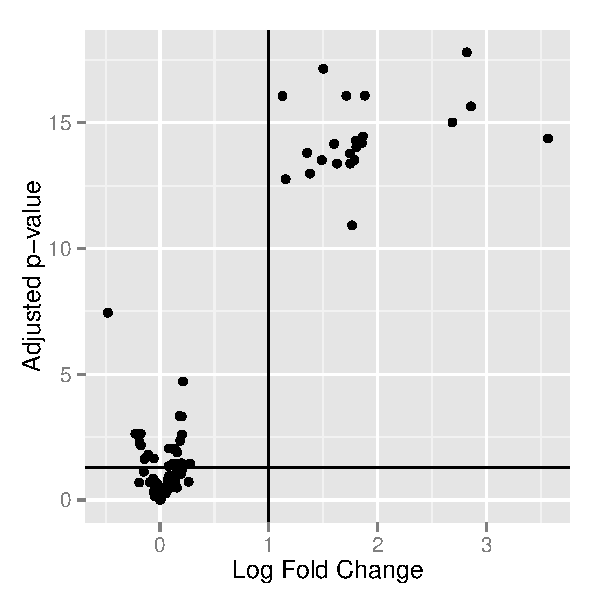
\includegraphics[width=6cm]{volcano.pdf}
\caption{Volcano plot showing differential gene expression.}
\label{F:volcano}
\end{centering}
\end{figure}

\begin{table}[H]
\begin{centering}
\begin{tabular}{cccc}
  \hline
Rank & Probe No & Probe ID & Log Fold Change \\ 
  \hline
1 &  74 & 202411\_at & 3.56 \\ 
  2 &  78 & 204439\_at & 2.86 \\ 
  3 &  77 & 214059\_at & 2.82 \\ 
  4 &  76 & 213797\_at & 2.69 \\ 
  5 &  75 & 204415\_at & 1.88 \\ 
  6 &  83 & 205483\_s\_at & 1.86 \\ 
  7 &  85 & 218400\_at & 1.85 \\ 
  8 &  89 & 227609\_at & 1.80 \\ 
  9 &  86 & 219863\_at & 1.80 \\ 
  10 &  80 & 202145\_at & 1.78 \\ 
  11 &  84 & 203153\_at & 1.76 \\ 
  12 &  79 & 219211\_at & 1.75 \\ 
  13 &  81 & 202869\_at & 1.74 \\ 
  14 &  90 & 204747\_at & 1.71 \\ 
  15 &  87 & 202086\_at & 1.63 \\ 
  16 &  91 & 204972\_at & 1.60 \\ 
  17 &  93 & 241916\_at & 1.50 \\ 
  18 &  88 & 205569\_at & 1.49 \\ 
  19 &  92 & 219684\_at & 1.38 \\ 
  20 &  82 & 44673\_at & 1.35 \\ 
  21 &  94 & 241812\_at & 1.15 \\ 
  22 &  33 & 212418\_at & 1.13 \\ 
   \hline
\end{tabular}
\caption{Differentially expressed genes using a cut off of $\alpha=0.05$ and log fold change $\ge 1$. In all cases FDR adjusted $p$-values were $\le$ 0.001} 
\label{T:GEGD}
\end{centering}
\end{table}

\begin{table}[h]
\centering
\begin{tabular}{ccc}
  \hline
Rank & ProbeNo & ProbeID \\ 
  \hline
1 &  33 & 212418\_at \\ 
  2 &  93 & 241916\_at \\ 
  3 &  75 & 204415\_at \\ 
  4 &  77 & 214059\_at \\ 
  5 &  62 & 222351\_at \\ 
  6 &  78 & 204439\_at \\ 
  7 &  79 & 219211\_at \\ 
  8 &  90 & 204747\_at \\ 
  9 &  76 & 213797\_at \\ 
  10 &  86 & 219863\_at \\ 
  11 &  74 & 202411\_at \\ 
  12 &  89 & 227609\_at \\ 
  13 &  94 & 241812\_at \\ 
  14 &  81 & 202869\_at \\ 
  15 &  92 & 219684\_at \\ 
  16 &  85 & 218400\_at \\ 
  17 &  88 & 205569\_at \\ 
  18 &  80 & 202145\_at \\ 
  19 &  83 & 205483\_s\_at \\ 
  20 &  91 & 204972\_at \\ 
   \hline
\end{tabular}
\caption{The top 20 genes which vary the most between the lupus sources and controls.} 
\label{T:DEGT}
\end{table}


\section{Summary}
The exploratory analysis suggested the following: 

\begin{enumerate}
\item There is strong evidence for differential gene expression between lupus patients and controls.
\item There is strong evidence for differential gene expression between different lupus sources. This is of secondary interest and might be due to some technical difference between samples, for example batch effects. Due to the small sample sizes which arise from classifying by source, the potential effect of source was not analysed further.

\item Genes show very strong linear associations and linear based techniques appear to describe the data well.
\item Both $A$ and $dcor$ appear to capture the linear relationships well.
\item $A$ and $dcor$ appear to differ in the relative importance of pairwise variable relationships.
\item LDA has less discriminatory power than FDA on the training dataset. The misclassification rate of FDA was only very slightly improved by allowing interactions to be considered.
\item MDS using $A$ or $dcor$ as a distance metric is a potential useful way to try to visualise variables in larger datasets.
\end{enumerate}

\chapter{Measuring Association: The Training Data}

\section{Two-way Associations}

\subsection*{Methods}
All two-way associations in the training dataset were analysed using $R^2$, $A$, $MIC$ and $dcor$ separately for lupus patients and controls. All two-way residual associations using $A$, $dcor$ and $MIC$ for lupus patients and controls were also calculated separately. This was performed as follows:

\begin{enumerate}

\item Fit a linear linear model of the form $Y = \beta_0 + \beta_1X + \epsilon$
\item Calculate the residual associations between $Y$ and $X$ as $A(\epsilon, X)$, $dcor(\epsilon, X)$ and $MIC(\epsilon, X)$.

\end{enumerate}

All association and residual association values were analysed visually and using rank based methods to assess if differences exist between lupus patients and controls and between each measure of association. The predictive power of strongly associated gene pairs was assessed by measuring their classification performance when used as explanatory variables in a MARS model where the response was disease status. For contrast the results were also compared to variable selection using MARS, this is given in Section 5.3.

 For results that were deemed significant, robust estimates of the association coefficients, $\hat{\theta}$, with associated standard errors were estimated using bootstrapping as follows:

\begin{enumerate}

\item For each $X$, $Y$ pair.
\item Sample $n$ data points with replacement from the observed data $z = \{ (x_1,y_1),...,(x_n,y_n) \}$ to get new data $z^*$.
\item Evaluate the sample association $\hat{\theta}^*$ of $z^*$.
\item Repeat steps 2 and 3 to obtain $\hat{\theta}_1^*,...,\hat{\theta}_{1000}^*$
\item Estimate the robust estimate of $\hat{\theta}$ by the mean of $\hat{\theta}_1^*,...,\hat{\theta}_{1000}^*$.
\item Estimate the standard error of $\hat{\theta}$ by the standard deviation of $\hat{\theta}_1^*,...,\hat{\theta}_{1000}^*$.

\end{enumerate}

\subsubsection{Testing Differences between Independent Associations}
The associations were calculated separately for lupus patients and controls meaning that they are from independent samples and that the difference in association between the two samples may be tested. In the case of correlations the difference in correlation between two independent samples could be tested using Fisher's $r$ to $z$ transformation.  In the case of the associations under study a non-parametric alternative is required, so a sign test based on bootstrapped estimates of the associations was used to estimate the significance of an observed difference as follows:

\begin{enumerate}

\item For each pair $X_L$, $Y_L$ and $X_C$, $Y_C$ in samples $L$ and $C$.
\item Sample $n=1000$ data points with replacement from the observed data $z_L = \{ (x_{L1},y_{L1}),...,(x_{Ln},y_{Ln}) \}$ and $z_C = \{ (x_{C1},y_{C1}),...,(x_{Cn},y_{Cn}) \}$ to get new data $z_L^*$ and $z_C^*$.
\item Evaluate the sample association $\hat{\theta_L}^*$ of $z_L^*$ and $\hat{\theta_C}^*$ of $z_C^*$.
\item Repeat steps 2 and 3 to obtain $\hat{\theta_{L1}}^*,...,\hat{\theta_{L1000}}^*$ and $\hat{\theta_{C1}}^*,...,\hat{\theta_{C1000}}^*$
\item Let $p$ be the probability that $\hat{\theta^*}_{Li} \ge \hat{\theta^*}_{Ci}$. Estimate the $p$-value of the difference in association using a sign test of the hypothesis: $H_0: p = 0.5$ against the two-sided alternative $H_1: p \ne 0.5$. 

\end{enumerate}
\subsection*{Results}
The distributions of each association can be seen in the box plots in Figure \ref{F:associationBox} which show positively skewed distributions in all cases. Both $dcor$ and $MIC$ show the greatest apparent differences in lupus patients and controls as measured by the inter-quartile range (IQR). All measures showed higher associations in controls than lupus patients however some very strong associations are present in lupus patients. The plots suggest general agreement between the different measures with stronger associations in lupus patients. The most obvious difference are the low level association recorded by both $dcor$ and $MIC$ however these are unlikely to be of interest. Obviously the rank order of the pairwise relations may differ meaning this has to be assessed by other means.

In all cases two-sided Wilcoxon rank sum tests provided overwhelming evidence that the distributions have different locations.

\begin{figure}[H]
\begin{center}
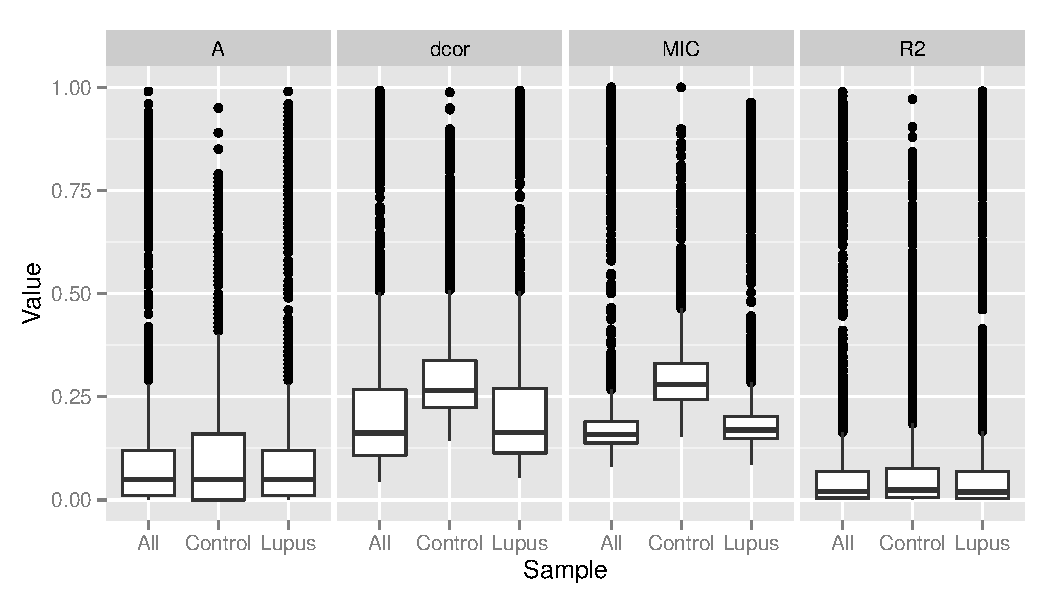
\includegraphics[width=\textwidth]{associationBox.pdf}
\caption{Boxplots of each association measure for all samples and then separately for controls and lupus patients.} 
\label{F:associationBox}
\end{center}
\end{figure}

\subsubsection{Comparison of the Association Estimates}
Bland-Altman \cite{Altman1983} plots (see Figure \ref{F:baTwoway}) were used to visually assess if any systematic differences existed between the measures and also to see if any bias as a result of the sample sample size was identifiable. Comparisons were made of each measurement type separately for lupus patients and controls. The red lines in each plot represent the 95\% limits of agreement between each measurement pair. 

The measures show less agreement in controls but this probably reflects the smaller sample sizes. The plots suggest that $MIC$ has the least agreement with the other measures. $A$, $dcor$ and $R^2$ appear to show reasonable agreement  as measured by the 95\% intervals although $dcor$ appears to have a systematic upward bias compared to $A$ and $R^2$. There are  no major differences between $R^2$ and either $A$ or $dcor$ which might suggest strong non-linear relationships. There appears to be little agreement in residual association as measured by $A$, $dcor$ and $MIC$.

\begin{figure}[H]
\begin{center}
\includegraphics[width=\textwidth]{mdAssociations2.pdf}
\caption{Bland-Altman plots comparing each association measure separately for controls and lupus patients.} 
\label{F:baTwoway}
\end{center}
\end{figure}


\subsubsection{Rank Comparison}
The absolute ranks of the computed associations were compared using two rank based correlation measures, Kendall's $\tau$ and Spearman's $\rho$. Ignoring ties, Kendall's $\tau$ is given by:
\[
\tau = \frac{n_c - n_d}{\frac{1}{2}n(n-1)}
\]

where $n_c$ is the number of concordant pairs, $n_d$ is the number of discordant pairs. This has an intuitive interpretation as the proportion of concordant pairs minus the proportion of discordant pairs making it attractive as a measure of association in contrast to Spearman's $\rho$ which is less easy to interpret but has other advantages. Kendall's $\tau$ is less sensitive to the effect of a few large differences in ranks when most pairs have the same rank. In general $\tau < \rho$ but Spearman's $\rho$ may heavily penalise large discordances (due to the $D^2$ term in the numerator) and hence is better suited to detecting one or two major discrepancies, for example if a $dcor$ value of 0.99 for a pair of genes vs. a $R^2$ value of 0.1 for the same pair \cite{Kendall}. 

In this case, $\tau < \rho$ for all measures in both samples and controls suggesting that there were no major discordances between the measures. The bar chart in Figure \ref{F:kendall} shows the results  for Kendall's $\tau$. In general the pattern is the same in both patients and controls although there are more discordances in controls, possibly a side effect of the smaller sample size. The most concordant measures are $R^2$ and $dcor$ while the most discordant are $R^2$ and $MIC$ possibly due to $MIC$'s lower power in detecting linear relationships. The residual associations were more discordant in all cases.

\begin{figure}[H]
\begin{centering}
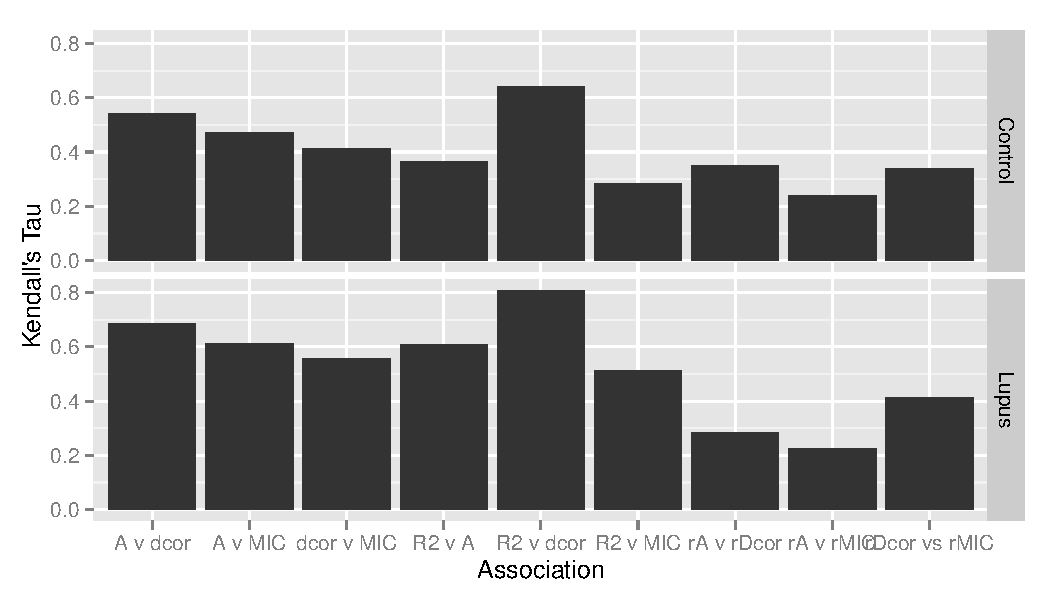
\includegraphics[width=\textwidth]{kendall2.pdf}
\caption{Bar charts showing rank correlation comparisons based on Kerndall's $\tau$.} 
\label{F:kendall}
\end{centering}
\end{figure}

\subsubsection{Strong Associations}
The main interest is in stronger associations so the results were grouped into the following levels: $\ge 0.01, \ge 0.05, \ge 0.10$. Within these levels discordances may exist but this is of secondary interest.

\begin{figure}[H]
\begin{centering}
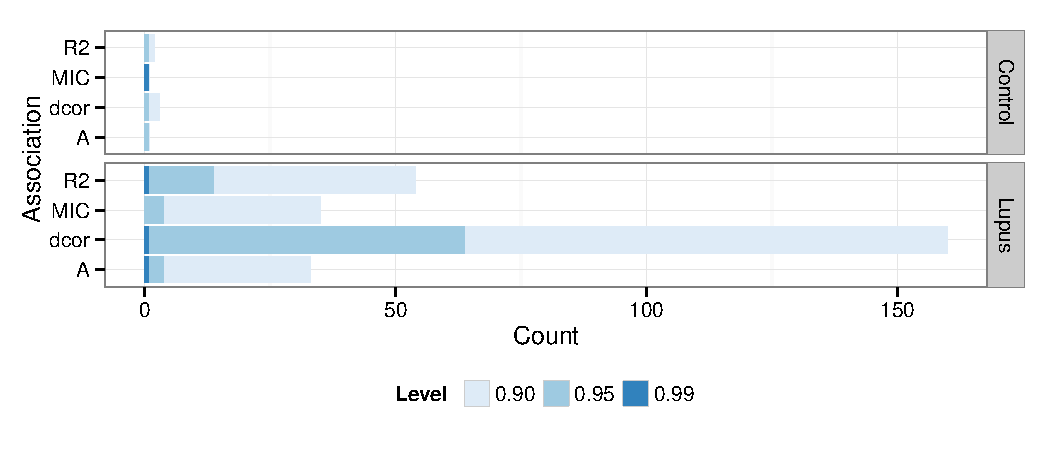
\includegraphics[width=\textwidth]{associationLevels.pdf}
\caption{Bar charts comparing the counts for each association measure at levels $\ge 0.90$, $\ge 0.95$ and $\ge 0.99$ separately for controls and lupus patients.} 
\label{F:levels}
\end{centering}
\end{figure}

Figure \ref{F:levels} shows the results of each association measure separately for lupus and controls. The most striking feature is that there are much stronger pairwise associations in lupus patients than controls. Within lupus patients only 2 values $\ge 0.99$ were recorded (one by $R^2$ and one by $dcor$), while $MIC$ scored one pair at this level in the control group. $A$ scored only 38 relationships $\ge 0.90$ in lupus patients compared with 160 in the case of $dcor$. $MIC$ had similarly low counts to $A$ in lupus patients.

Three pairwise relationships, (Probe No 30:31, 86:76, 42:41) formed the intersection of the associations $\ge 0.90$ for both samples. Plots (not shown) revealed that these had very strong linear relationships and were identified by all association measures. These associations also occurred in lupus patients, with strong ($\ge 0.95$) scores by all association measures. Of these probes, only probe number 86 (219863\_at) was differentially expressed. Because they occurred in both patients and controls they are unlikely to be of interest and hence can be excluded from further consideration. 

The Venn diagrams in Figure \ref{F:Venn} shows that $dcor$ is the union of the other association measures and that both $MIC$ and $A$ miss a large number (17 and 24 respectively) number of linear relationships. Clearly large differences exist between $dcor$ and both $A$ and $MIC$. 

\begin{figure}
    \centering
    \subfloat[Controls]{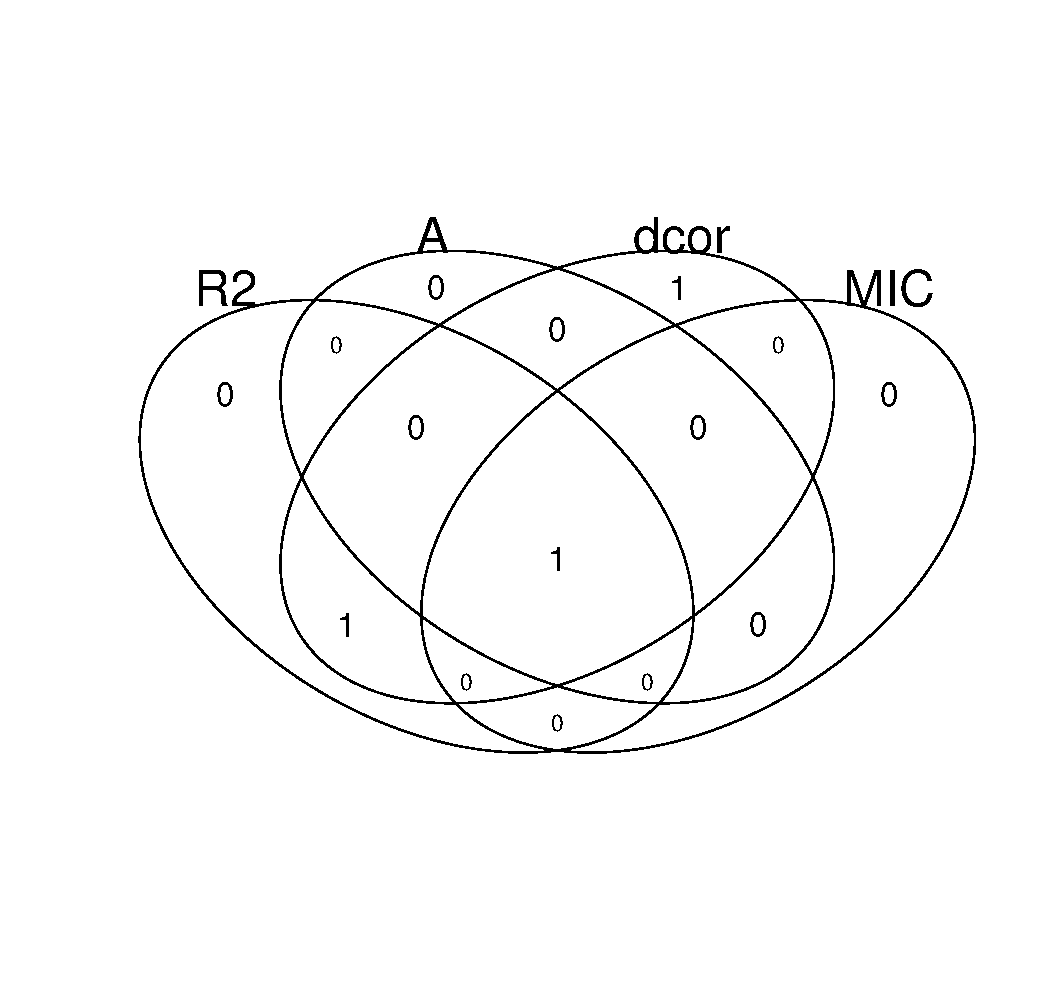
\includegraphics[width=7cm]{vennControl.pdf} }
    \qquad
    \subfloat[Lupus]{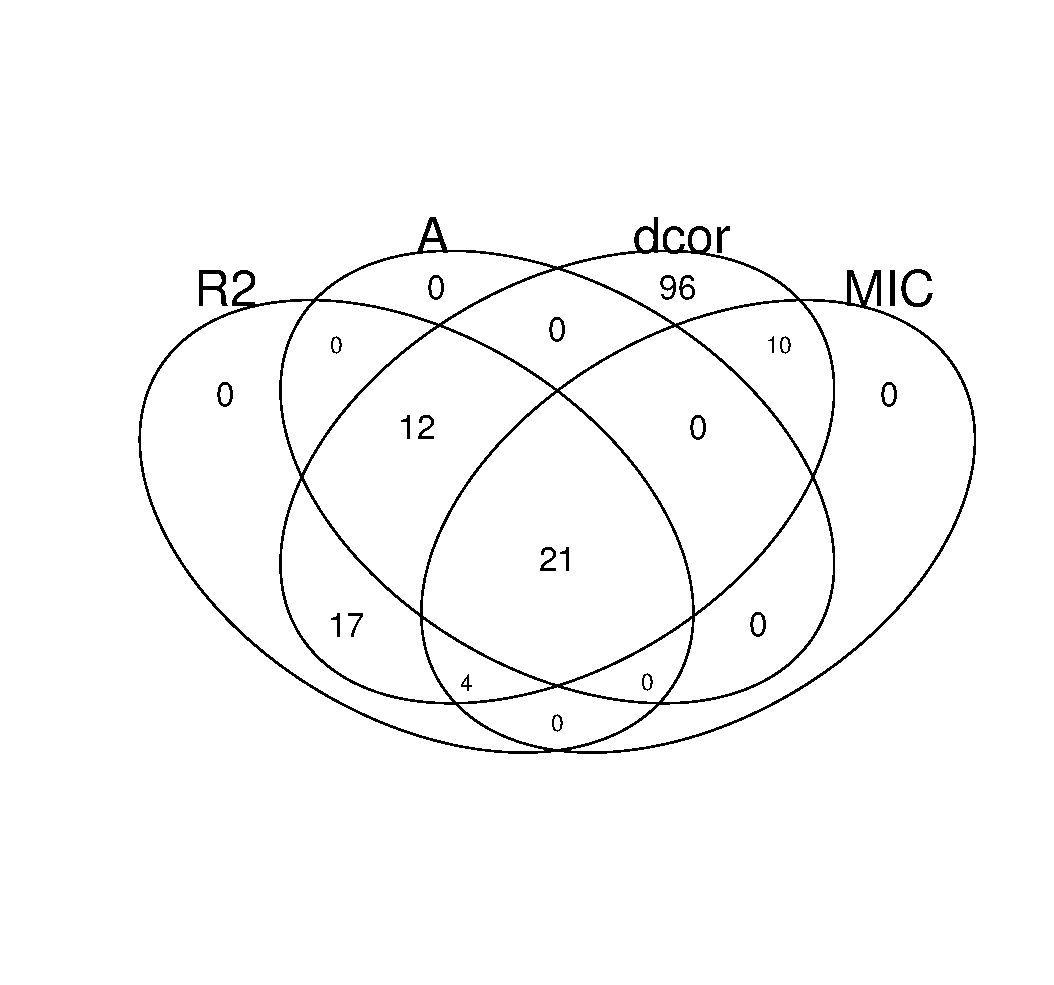
\includegraphics[width=7cm]{vennLupus.pdf} }
    \caption{Venn diagrams showing associations $\ge 0.90$.}
    \label{F:Venn}
\end{figure}

\subsubsection{Non-Linearity}
The Bland-Altman plots and Kendall's correlation showed that there was very little agreement between the $A$, $dcor$ and $MIC$ based on residual association. In particular, $A$ and $MIC$ based residual association tended to be higher but these pairs also had strong $R^2$ values. This suggests that $dcor$ may potentially produce more stable results for non-linear association mining, in that it produced consistently low values for both residual and partitioned association however further analysis would be needed to verify this.

Kendall's correlation of the residual association and non-linear part of association also showed low concordance within each measure (0.46, 0.37, 0.12 for $A$, $dcor$ and $MIC$ respectively). Rounding the results to 2 d.p. only resulted in very small increases ($\approx$ 0.02) in Kendall's $\tau$. The likely explanation for this is that the main extant two-way relationships are linear in nature meaning that the residual association is very noisy and that there is too little remaining signal for each measure too detect.  This suggests that where associations are suspected to be primarily linear in nature or have a strong linear component, partitioning based assessments of non-linearity are preferable to residual association.

Of the partitioned methods some differences in the ranks given by the non-linear part of association and non-linear proportion of association naturally exist but taken within a predefined threshold level such as $dcor \ge 0.90$ these were minor and made no qualitative difference in the case of the lupus dataset. Both $A$ and $MIC$ missed many of the linear associations, hence their partitioned non-linearity results are discordant with those of $dcor$.

\subsubsection{Filtering}
The preceding results can be combined to filter the results into associations of potential interest based on three criteria: $\alpha$, the desired strength of association, $\beta$, the amount of non-linearity and $\gamma$, the difference in association between lupus patients and controls. The results in Figure \ref{F:2wayTop} are based on the following formula:

\[
(X_i, Y_i) = \{\theta_{lupus} \ge \alpha\} \cap \{(\theta_{lupus} - R^2_{lupus}) \ge \beta \} \cap \{\theta_{lupus} - \theta_{control} \ge \gamma \}
\]

where $X_i$ and $Y_i$ are probes of interest, $i \in \{1, ..., 94\}$, the association measure $\theta = dcor$, $\alpha$ the required association level $\ge 0.90$, $\beta$, the required non-linear part of association $\ge 0.1$ and $\gamma$, the required difference in association between lupus and controls $\ge 0.45$. The results were then ordered by non-linear part of association. The sign test for differences in association were highly significant in all cases (estimated $p$-value $<$ 0.001).

Based on this criteria the analysis found 18 pairwise association of interest consisting of different 15 probes. Of these all were differentially expressed and had a log-fold change $\ge 1$. The 15 probes mapped to the following 15 genes on 11 different chromosomes: IFI27,  Hs.82316, IFI44L   LY6E, OAS1. SIGLEC1, ISG15, IFIT1, OAS3, MX1, LAMP3, EPSTI1, IFIT3, RTP4  and SPATS2l.  

The chosen threshold values are somewhat arbitrary and primarily illustrative but could obviously be varied according to need or domain expertise or encompass additional criteria such as differential expression. It is important to note that a large difference in association  between lupus patients and controls does not mean that the difference is statistically significant and conversely a statistically significant difference in association does not imply biological importance. 
 
All of these relationships were well described by linear methods such as Pearson correlation as can be seen in Figure \ref{F:2wayTop} which shows scatter plots of the eighteen  associations identified by $dcor$. Each plot shows lupus patients in blue and controls in red. Smoothed lines describing the relationship were fitted separately using a form of locally weighted regression called loess \cite{MASS}. The bands represent 95\% confidence intervals. The plots show some suggestion of quadratic or sigmoid relationships but these are modest and consistent with the non-linear part of association which varies from 0.15 to 0.10. 

Table \ref{T:2wayAssociations} compares the corresponding association values based on bootstrapped estimates of each measure (see Section 5.1 for the method used). An interesting aspect of these results is that the robust estimates of $A$ and $MIC$ are closer to $dcor$ than the point estimates were. A possible explanation for this is that $A$ and $MIC$ are more sensitive to outliers than $dcor$ which has very low estimated standard deviation. Simulation could be used to explore this further in a future study. The estimated standard deviation of $MIC$ appears higher than that of either $A$ or $dcor$.




\begin{figure}[H]
\begin{centering}
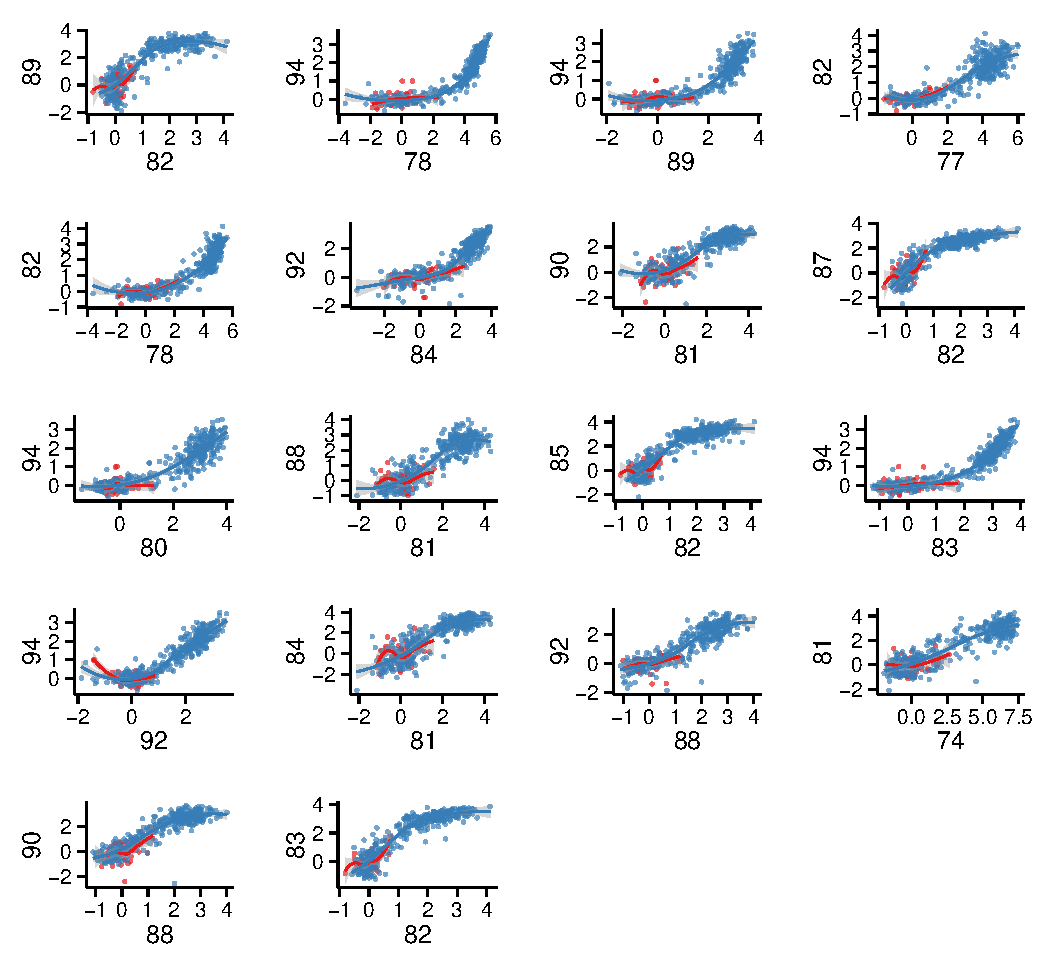
\includegraphics[width=\textwidth]{2wayTop.pdf}
\caption{Scatter plots showing eighteen two-way associations where $dcor_{lupus} \ge 0.90$ and $dcor_{lupus} - R^2_{lupus} \ge 0.10$ and $dcor_{lupus} -dcor_{control} \ge 0.45$. The plots are in decreasing order  by $dcor_{lupus} - R^2_{lupus}$} 
\label{F:2wayTop}
\end{centering}
\end{figure}

\begin{table}[h]
\begin{centering}
\begin{tabular}{cccccccccc}%rrrrrrrrrrr
  \hline
  X & Y & $dcor$ & $\sigma_{dcor}$ & $R^2$ & $\sigma_{R^2}$ & $A$ & $\sigma_{A}$ & $MIC$ & $\sigma_{MIC}$ \\ 
  \hline
 82 & 89 & 0.906 & 0.008 & 0.758 & 0.016 & 0.920 & 0.013 & 0.885 & 0.035 \\ 
 78 & 94 & 0.910 & 0.008 & 0.771 & 0.017 & 0.941 & 0.010 & 0.971 & 0.018 \\ 
 89 & 94 & 0.905 & 0.008 & 0.766 & 0.017 & 0.924 & 0.013 & 0.924 & 0.030 \\ 
 77 & 82 & 0.902 & 0.010 & 0.766 & 0.019 & 0.926 & 0.013 & 0.885 & 0.038 \\ 
 78 & 82 & 0.921 & 0.007 & 0.792 & 0.014 & 0.927 & 0.012 & 0.902 & 0.032 \\ 
  84 & 92 & 0.907 & 0.009 & 0.791 & 0.023 & 0.932 & 0.012 & 0.910 & 0.038 \\ 
 81 & 90 & 0.917 & 0.008 & 0.802 & 0.022 & 0.929 & 0.013 & 0.883 & 0.040 \\ 
 82 & 87 & 0.915 & 0.008 & 0.801 & 0.014 & 0.930 & 0.012 & 0.888 & 0.031 \\ 
 80 & 94 & 0.910 & 0.010 & 0.801 & 0.015 & 0.919 & 0.013 & 0.903 & 0.036 \\ 
  81 & 88 & 0.908 & 0.009 & 0.801 & 0.016 & 0.925 & 0.013 & 0.863 & 0.041 \\ 
  82 & 85 & 0.924 & 0.007 & 0.819 & 0.014 & 0.924 & 0.012 & 0.893 & 0.036 \\ 
  83 & 94 & 0.924 & 0.007 & 0.818 & 0.013 & 0.938 & 0.009 & 0.948 & 0.023 \\ 
  92 & 94 & 0.938 & 0.008 & 0.833 & 0.021 & 0.934 & 0.011 & 0.961 & 0.020 \\ 
  81 & 84 & 0.905 & 0.010 & 0.799 & 0.018 & 0.928 & 0.013 & 0.867 & 0.037 \\ 
  88 & 92 & 0.913 & 0.009 & 0.808 & 0.020 & 0.925 & 0.013 & 0.879 & 0.043 \\ 
  74 & 81 & 0.908 & 0.011 & 0.806 & 0.019 & 0.927 & 0.013 & 0.881 & 0.041 \\ 
  88 & 90 & 0.929 & 0.009 & 0.827 & 0.031 & 0.926 & 0.013 & 0.862 & 0.042 \\ 
  82 & 83 & 0.930 & 0.007 & 0.829 & 0.013 & 0.931 & 0.011 & 0.906 & 0.033 \\ 
   \hline
\end{tabular}
\caption{Bootstrap estimates of the eighteen two-way associations along with the corresponding estimates of standard deviation. $X$ and $Y$ refer to probes in two-way associations.} 
\label{T:2wayAssociations}
\end{centering}
\end{table}

\subsubsection*{Multiple Adaptive Regression Splines}
MARS models were used as a way to contrast the association results with a classification method. MARS allow binary classification by fitting an adapted logistic regression model but allows the explanatory variables to enter as curved linear basis functions called `hinge' functions and so can handle non-linearity \cite{earth}. A useful feature of MARS models is that the explanatory terms can also be treated linearly and hence the difference in results between linear and non-linear models provides some additional insight into how non-linear relationships may be important for lupus. 

For each of the associations of interest identified, MARS models were built and their goodness of fit was measured. One criterion for assessing the goodness of fit of a MARS model is Generalised Residual Sum of Squares (GRSq, an approximation of RSS that would be measured on independent data, further criteria for interpreting MARS models are given in Section 5.3).  For each of the eighteen two-way associations the GRSq for a linear and non-linear MARS models was calculated. Figure \ref{F:GRSqvAssociation} shows the relationship of associations $\ge 0.90$ against the corresponding MARS model. It shows that by themselves the probe pairs are poor classifiers of lupus but that using `hinge' functions produces a very modest improvement in GRSq in all cases. This is therefore consistent with the results of the two-way association analysis indicating that linear relationships are dominant. It also illustrates the important distinction between association and causation, i.e. the fact that random variables are associated does not imply a causal relationship.

\begin{figure}[H]
\begin{centering}
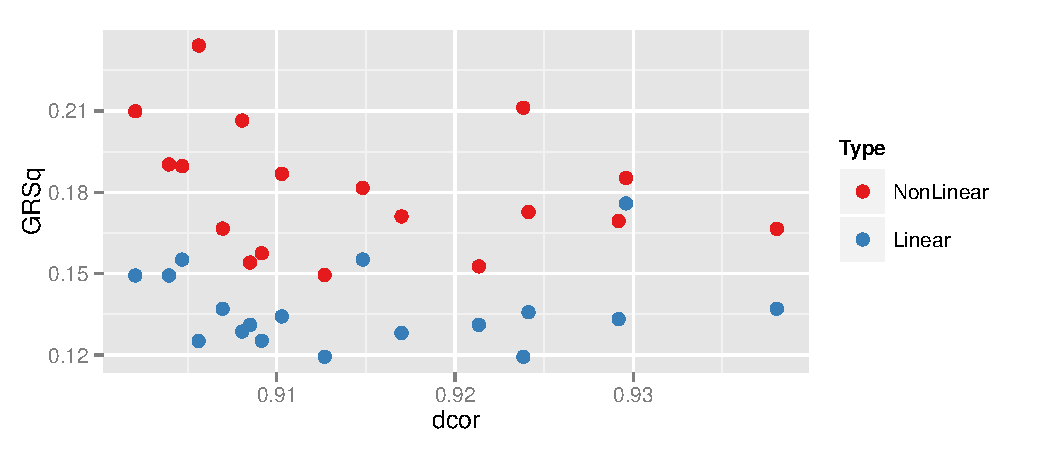
\includegraphics[width=\textwidth]{grsqVdcor.pdf}
\caption{MARS based GRSq vs association for the 18 two-way associations of interest.} 
\label{F:GRSqvAssociation}
\end{centering}
\end{figure}

\section{Three-way Associations}
The method for analysing three-way relationships followed that used for two-way associations with the following two exceptions:

\begin{enumerate}
\item Only $R^2$, $dcor$ and $A$ extend to the multivariate case so all three way combinations were compared using each of these association measures. $MIC$ can only handle pairwise relationships so could not be included.
\item $R^2$ was calculated by fitting a linear model allowing interaction of the two explanatory variables, i.e. $Y= \beta_0 +\beta_1X+ \beta_2Z+ \beta_{1,2}X  Z$. 
\end{enumerate}

The number of possible three way relationships for the training dataset is $\frac{1}{2}(_{94} P_{3})=402132$, making the analysis computationally expensive but still tractable given that there were only 94 variables. This allowed for asymmetry in the associations, i.e. for some association function $\theta$; $\theta(X:Y,Z) \ne \theta(Y:X,Z) \ne \theta(Z:X,Y)$, but did not allow duplicates caused by the fact that $\theta(X:Y,Z) = \theta(X:Z,Y)$.

\subsection*{Results}
The boxplots in Figure \ref{F:3wayBox} show the distributions of each association measure. They show that $dcor$ has higher IQR values than either $A$ or $R^2$ as in the two-way case but that all measures show some very strong three-way associations. The range of $A$ based residual association is again greater than that of $dcor$. The Bland-Altman plots in Figure \ref{F:3wayBA} suggests generally moderate agreement between $A$ and $R^2$ but better agreement for very strong associations. $dcor$ is again biased upwards from both $A$ and $R^2$ (median values for lupus patients were 0.21, 0.07 and 0.09 respectively). There appears to be little agreement between $A$ and $dcor$ based on residual association. 

\begin{figure}[H]
\begin{centering}
\includegraphics[width=\textwidth]{3wayBox.pdf}
\caption{Boxplots of each association measure for controls and lupus patients.} 
\label{F:3wayBox}
\end{centering}
\end{figure}

\begin{figure}[H]
\begin{centering}
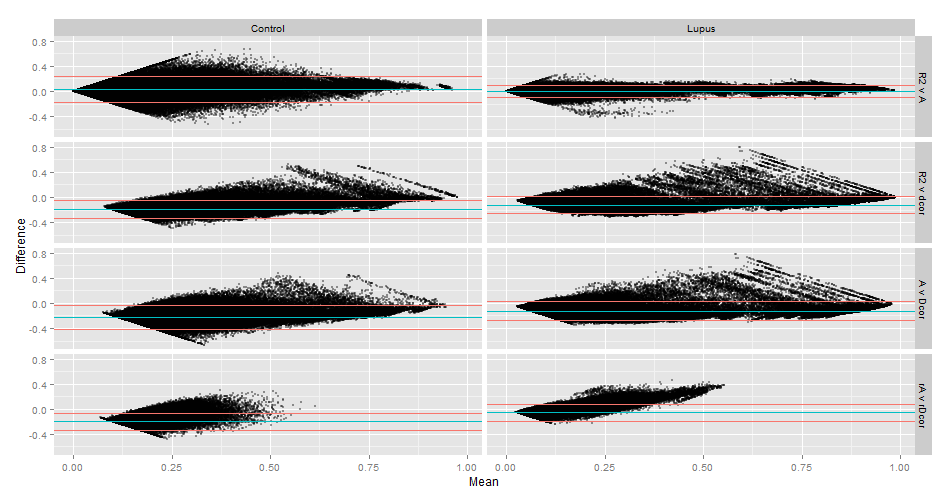
\includegraphics[width=\textwidth]{3wayBA.png}
\caption{Bland-Altman plots of controls and lupus patients for each association measure.} 
\label{F:3wayBA}
\end{centering}
\end{figure}

The bar chart in Figure \ref{F:3wayKendall} suggests greater discordance in the three-way case than the two way case, but given the number of associations being measured the decrease in concordance is unsurprising. Of the pairs, $R^2$ and $dcor$ still are most concordant while the residual associations are most discordant. As in the two-way case Spearman's $\rho$ was greater than Kendall's $\tau$ for all pairs implying that there were no major discordances.

\begin{figure}[H]
\begin{centering}
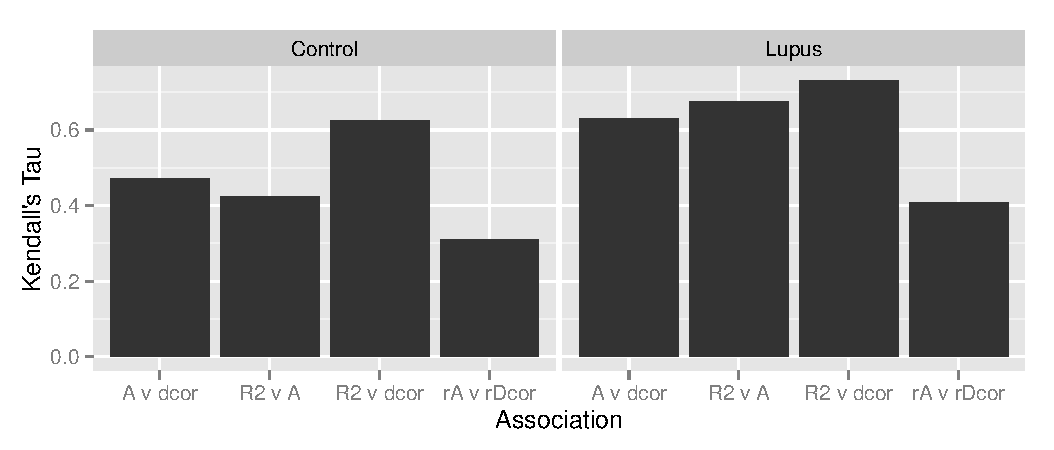
\includegraphics[width=\textwidth]{3wayKendall.pdf}
\caption{Kendall's $\tau$ comparing ranks of three-way associations.} 
\label{F:3wayKendall}
\end{centering}
\end{figure}

The barcharts in Figure \ref{F:3wayLevels} show the associations at the $\ge 0.90$, $\ge 0.95$ and $\ge 0.99$ levels. Again the picture is similar to the two-way case with the majority of high level associations in lupus patients and $dcor$ having much higher values but $A$ having the fewest. The Venn diagram in Figure \ref{F:Venn3} shows that all association $\ge 0.90$ in both controls and lupus patients were found by the union of $dcor$ and $R^2$.  $dcor$ identified 58.0\% and 93.9\% of associations identified by $R^2$ in controls and lupus patients respectively, compared with 35.25\% and 27.19\% for $A$. This indicates that the power deficiencies of $A$ in identifying linear relationships extend to the three-way case. Ignoring the possibility of inflated false discovery by $dcor$, the analysis suggested that $A$ added no new information over the combination of $dcor$ and $R^2$.

\begin{figure}[H]
\begin{centering}
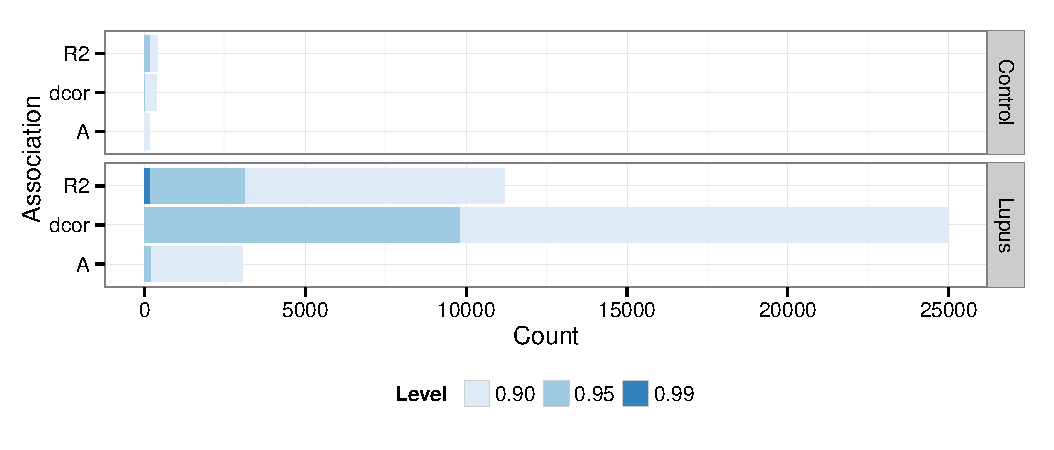
\includegraphics[width=\textwidth]{3wayLevels.pdf}
\caption{Three-way associations $\ge 0.90$.} 
\label{F:3wayLevels}
\end{centering}
\end{figure}

Four three-way relationships had $dcor > 0.99$ however all of these had $R^2 > 0.98$ and $A > 0.95$, suggesting that linear effects were dominant. Additionally three of the four associations involved probes 86 and 87 which were very highly correlated in both controls and lupus patients and therefore unlikely to be of interest. Most of the $dcor$ associations $\ge 0.95$ also had high $R^2$ values and contained all 94 probes. On average the non-linear difference $dcor -R^2$ was 0.03 with a standard deviation of $0.015$ indicating that $dcor$ was only detecting minor additional non-linear effects. 3D scatter plots (not shown) suggested that these were  well described by a plane. The residual association values for both $A$ and $dcor$ failed to identify any strong non-linear relationships. As with the two-way case $A$ based residual association seemed unreliable in that in that a high residual association value also had high $A$ and $R^2$ values.

\begin{figure}
    \centering
    \subfloat[Controls]{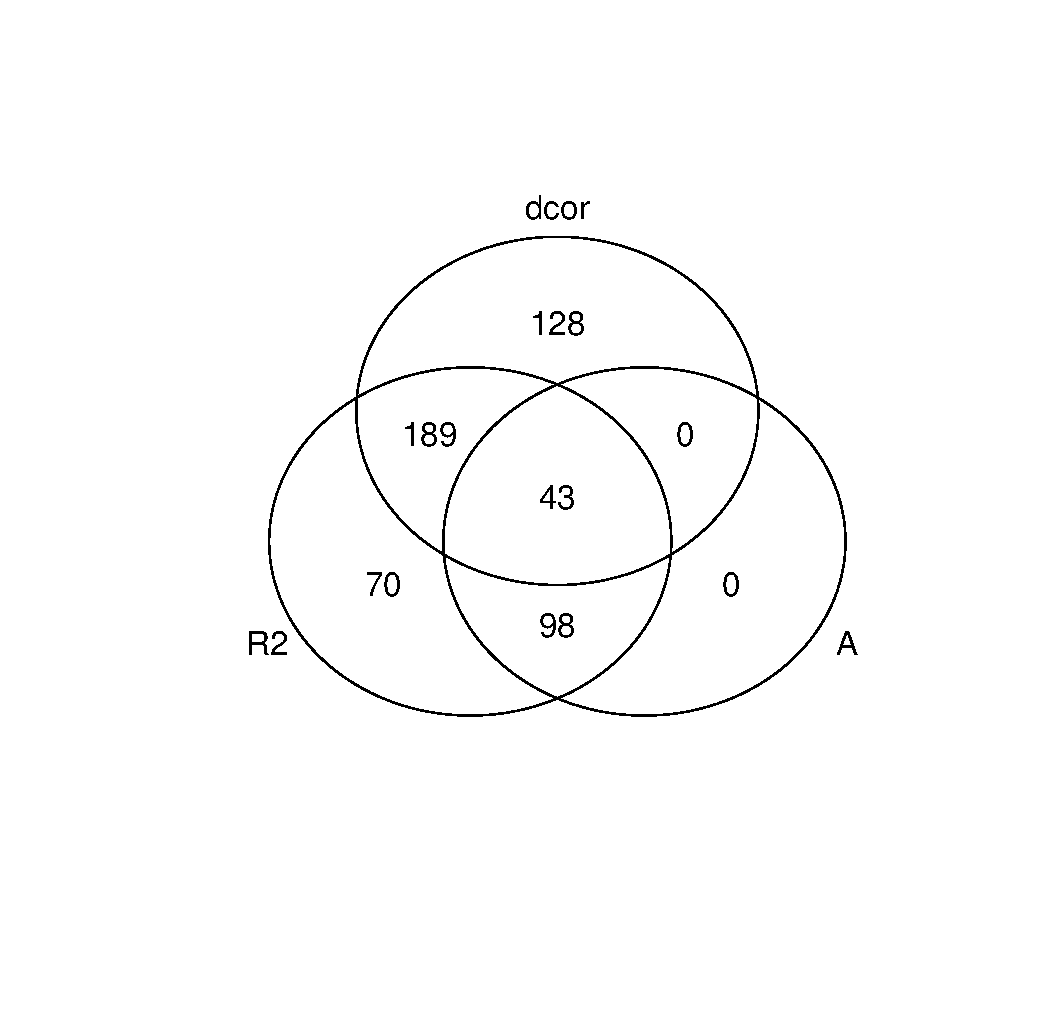
\includegraphics[width=7cm]{vennControl3.pdf} }
    \qquad
    \subfloat[Lupus]{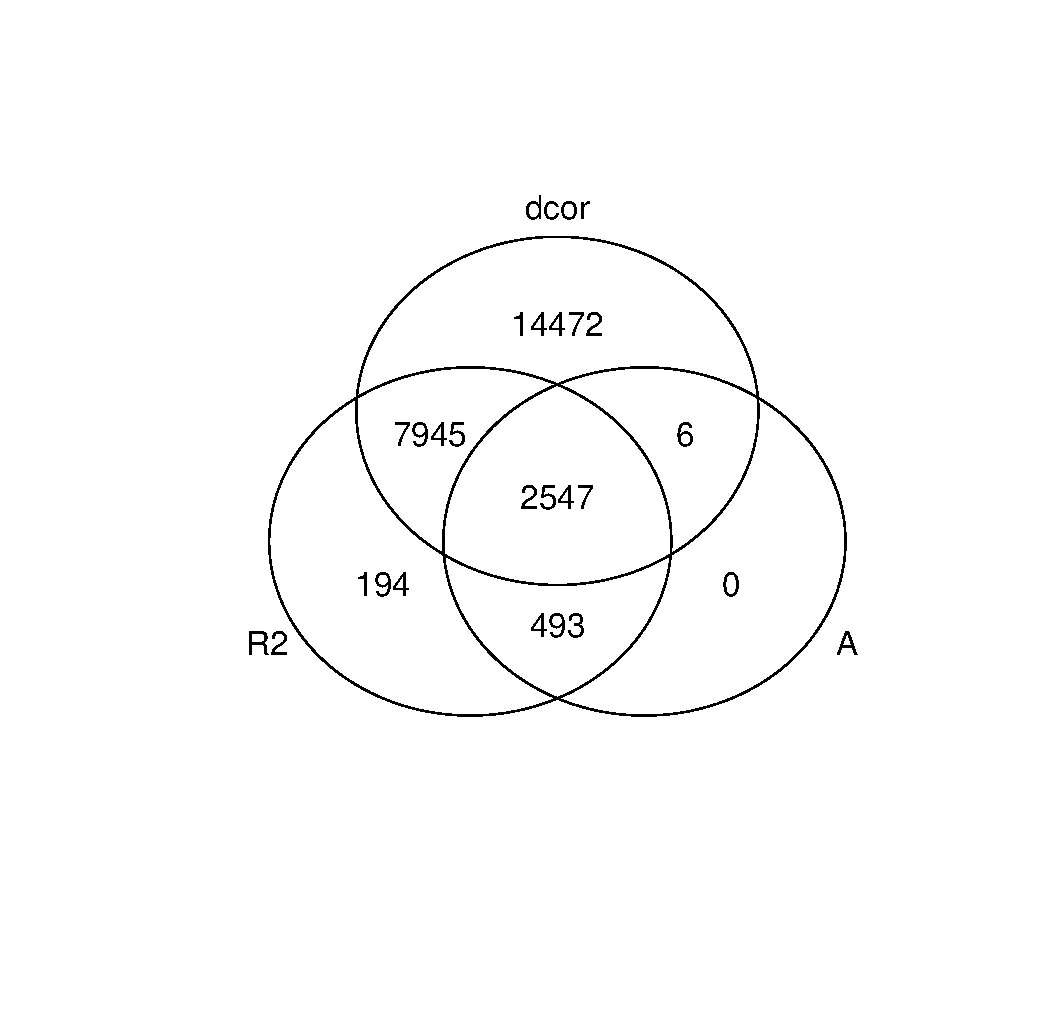
\includegraphics[width=7cm]{vennLupus3.pdf} }
    \caption{Venn diagrams showing three-way associations $\ge 0.90$.}
    \label{F:Venn3}
\end{figure}

\subsubsection{Filtering}
The number of strong three-way associations is problematic and is a consequence of the necessary increase in association caused by the addition of extra explanatory information provided by the third variable. For example, if two variables $X$ and $Z$ have a high two-way association as measured by $\theta(X, Z)$ then $\theta(X: Y,Z)$ and $\theta(Z: Y,X)$ will also be high. To mitigate this a more refined filtering strategy than that used in the two-way case is required. Figure \ref{F:3wayFilter} illustrates this by showing the effect of four different filtering strategies on the three-way association results. Each plot shows the amount of times a probe occurs in a three-way association. Plot A shows the three-way equivalent of the two-way filter from Section 5.2, i.e. it deems a three-way association to be of interest if the total association is large ($\alpha$), considerably different between lupus patients and controls ($\beta$), and the non-linear part of association is more than 10\% ($\gamma$), giving

\[
(X_i, Y_i, Z_i) = \{\theta_{lupus} \ge \alpha \} \cap \{ (\theta_{lupus} - R^2_{lupus}) \ge \beta \} \cap \{ \theta_{lupus} - \theta_{control} \ge \gamma \}
\]

However this results in 1044 associations of interest many of which contain probes 74 to 94 which have very strong pairwise associations while the addition of the third probe only causes a marginal increase in association. (In all cases there was overwhelming evidence ($p$-value $<$ 0.001) that there was a difference in association between the two samples.) Plot B imposes the additional constraint that probes from strong two-way associations are removed, this results in 168 associations. Plot C is the same as plot A but also filters for differentially expressed genes, yielding 12 associations. Plot D is the result of combining the previous 3 filter strategies resulting in a single three-way association of interest. The non-linear part of association is similar to the two-way case varying from 0.15 to 0.10 for these associations. 

As with the two-way case, these filters could be adapted on a needs basis. If it is the case that the sole interest is in differentially expressed genes then considerable computational effort could be avoided by only analysing the three-way associations of those genes.

\begin{figure}[H]
\begin{centering}
\includegraphics[width=15cmh]{3wayFilter.pdf}
\caption{Four different filter strategies for three-way associations with $dcor \ge 90$ \& $dcor - R^2 \ge 0.1$ \& $dcor_{lupus} - dcor_{control} \ge 0.45$. Each plot shows the frequency of probe involvement in a three-way association.} 
\label{F:3wayFilter}
\end{centering}
\end{figure}

\begin{figure}[H]
\begin{centering}
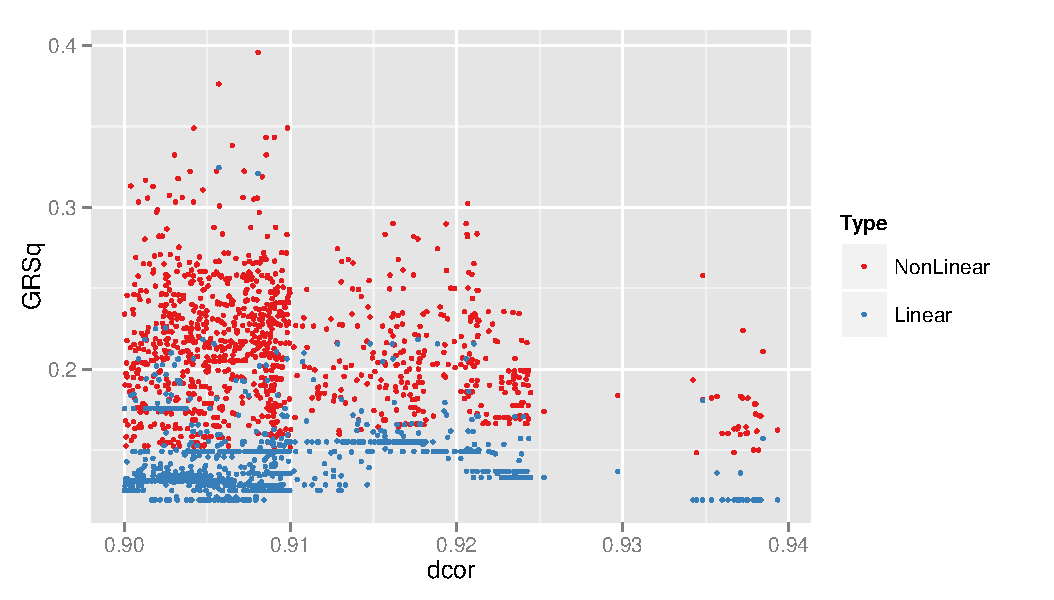
\includegraphics[width=\textwidth]{grsqVdcor3way.pdf}
\caption{MARS based GRSq vs association for the initial 1044 three-way associations of interest, corresponding to Figure \ref{F:3wayFilter} A.} 
\label{F:GRSqvAssociation3way}
\end{centering}
\end{figure}

\begin{table}[H]
\begin{centering}
\begin{tabular}{rrrrrrrrr}
  \hline
 X & Y & Z & $dcor$ & $\sigma_{dcor}$ & $R^2$ & $\sigma_{R^2}$ & $A$ & $\sigma_A$ \\ 
  \hline
82 &   77 &   88 & 0.910 & 0.009 & 0.792 & 0.018 & 0.997 & 0.001 \\ 
 82 &   33 &   78 & 0.908 & 0.008 & 0.794 & 0.015 & 0.998 & 0.001 \\ 
 92 &   74 &   82 & 0.903 & 0.011 & 0.790 & 0.023 & 0.997 & 0.001 \\ 
  82 &   88 &   89 & 0.909 & 0.008 & 0.798 & 0.018 & 0.996 & 0.002 \\ 
  92 &   74 &   75 & 0.904 & 0.011 & 0.796 & 0.024 & 0.998 & 0.001 \\ 
  82 &   89 &   93 & 0.903 & 0.009 & 0.794 & 0.018 & 0.997 & 0.001 \\ 
  92 &   82 &   93 & 0.909 & 0.009 & 0.803 & 0.022 & 0.998 & 0.001 \\ 
  82 &   89 &   92 & 0.912 & 0.009 & 0.809 & 0.019 & 0.996 & 0.001 \\ 
  82 &   77 &   89 & 0.911 & 0.008 & 0.808 & 0.019 & 0.996 & 0.001 \\ 
  74 &   88 &   92 & 0.902 & 0.012 & 0.801 & 0.020 & 0.997 & 0.001 \\ 
 74 &   77 &   92 & 0.905 & 0.011 & 0.805 & 0.018 & 0.997 & 0.001 \\ 
  81 &   33 &   74 & 0.906 & 0.010 & 0.807 & 0.019 & 0.998 & 0.001 \\ 
   \hline
\end{tabular}
\caption{Bootstrap estimates of the twelve three-way associations along with the corresponding estimates of standard deviation} 
\label{tabsmall}
\end{centering}
\end{table}

An additional consideration is the explanatory power of the associations of interest identified to predict disease status. MARS models were again used to assess this based on the model GRSq. In the three-way case the models were allowed the additional flexibility of three-way variable interactions. The results are shown in Figure \ref{F:GRSqvAssociation3way}. They suggest an average improvement in model fit (mean = 0.21) but that overall they have explained relatively little of the observed variability between lupus patient and controls. Using MARS `hinge' functions as opposed to linear predictors resulted in increased GRSq in all cases. On average the increase was modest at 0.07 (to 2 d.p.) with a standard deviation of 0.03, showing consistency with the two-way case.

Generally the results of the three-way analysis was similar to the two-way case, in that $dcor$ identified more relationships of interest than $A$ and was biased upwards from $R^2$. A possible explanation for this is that $dcor$ was able to detect the additional non-linear relationships present that were missed by $R^2$. $A$ missed many of the linear associations detected by $R^2$ suggesting that at the least it needs to be used in conjunction with either $R^2$ or $dcor$ for exploratory association analysis.

\section{Multiple Adaptive Regression Splines: Variable Importance}
A large association does not necessarily imply that it is a good predictor of lupus, this was the reason for using MARS to try to classify disease status on the basis of large associations in the previous sections. This section further explores the classification capacity of MARS and how they can be used to select important genes. The results provide additional contrast to the two and three-way association analyses and also investigate some differences between linear and non-linear modelling.

Six different MARS models were compared. Models were built allowing either no, two or three-way interactions, this is called the model degree. All genes were input as either non-linear MARS `hinge' functions or as linear predictors. The response variable was disease status so the underlying model was similar to logistic regression. All models were fitted using 10 step, 2 fold cross validation for robustness. The flexibility of MARS models makes them susceptible to over-fitting so stratified sampling was used to create a 70:30 split of training and test subsets (based on the training data reported on in this chapter). 

 The classification  performance of the the model can be assessed by measuring the Area Under the Curve (\gls{AUC}) of the Receiver Operating Characteristic (\gls{ROC}). The ROC is a graph of `sensitivity' (true positive rate) versus `specificity' (false positive rate). AUC takes values from 0 to 1. An AUC close to 1 indicates high classification accuracy (few false positives and negatives) while a random classifier would have an AUC of $\approx 0.5$. The ROCs of each model built on the training data and used to predict the test data are shown in Figure \ref{F:marsROC}. The results show that all models have mixed classification rates with AUCs of 0.90, 0.96, 0.84 for the non-linear models and 0.94, 0.90, 0.94 for the linear ones. If no variable interaction is allowed then the linear models have very slightly improved classification however the amount of permitted variable interaction appears to be more important in classification. The highest AUC is achieved by the two degree non-linear model but this is only a very marginal increase over the linear case. This result is consistent with the exploratory and association analyses which suggest that linear relationships well describe the lupus dataset. A refinement to the analysis would be to consider the relative costs of misclassifying disease status when evaluating model performance.

\begin{figure}[H]
\begin{centering}
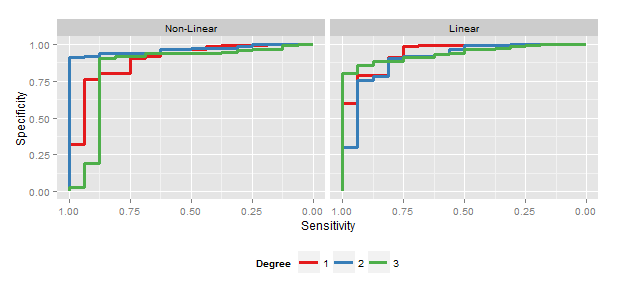
\includegraphics[width=\textwidth]{marsROC.png}
\caption{Receiver Operating Characteristics comparing six different MARS models allowing different levels of interaction and flexibility of the explanatory variables.} 
\label{F:marsROC}
\end{centering}
\end{figure}

\subsubsection{Variable Importance}
The fact that MARS allows different degrees of variable interaction makes it appealing for variable selection, however, as with other data mining techniques, ranking variable importance can be misleading in MARS, so the underlying selection process needs to be understood. 

MARS uses the following three criteria to assess variable importance: Residual Sum of Squares (RSS), Generalised Cross Validation (GCV, an approximation of RSS that would be measured on independent data) and the number of model subsets which contained the model. (GCV and GRSq are related statistics, GRSq normalises GCV in the same way that $R^2$ normalise RSS \cite{earth}). Variables which cause a large decrease in RSS and GCV are considered important and variables occurring in a large number of sub-models are also considered important. The final variable importance is a function of these three criteria. A particular problem with MARS can arise due to collinearity between predictor variables in which case the stepwise selection process can artificially inflate one predictors importance over another \cite{earth}. An additional problem is that is that variables which are considered important singly and also in an interaction may be given an artificially high weight. Hence the rankings in Table \ref{T:MARS} need to be evaluated with this in mind. One mitigation strategy is to use a process known as `bagging' to average out fitted models and the associated ranked predictors \cite{earth}. A consequence of this variable selection procedure is that the final rankings are on a per variable basis and not in terms of interactions. 

\begin{table}[H]
\begin{tabular}{ccccc}
  \hline
Probe No & MARS Rank & $dcor$ two-way & $dcor$ three-way & Differentially Expressed \\ 
  \hline
33 & 1  &  & 1 & Y \\ 
80 & 2  & 1 &  & Y \\ 
66 & 3  &  &  &  \\ 
75 & 4  &  & 1 & Y \\ 
89 & 5 & 2 & 2 & Y \\ 
84 & 6  & 2 &  & Y \\ 
 77 & 7  & 1 & 1 & Y \\ 
37 & 8  &  &  &  \\ 
 78 & 9  & 1 & 1 & Y \\ 
 68 & 10  &  &  &  \\ 
  5 & 11  &  &  &  \\ 
  14 & 12  &  &  &  \\ 
  38 & 13 &  &  &  \\ 
  73 & 14  &  &  &  \\ 
  53 & 15  &  &  &  \\ 
  83 & 16  & 2 &  & Y \\ 
  25 & 17 &  &  &  \\ 
  19 & 18  &  &  &  \\ 
  56 & 19 &  &  &  \\ 
  35 & 20  &  &  &  \\ 
   \hline
\end{tabular}
\caption{Comparison of MARS ranking of variable importance with the $dcor$ selected associations and differential expression results. $dcor$ two-way and three-way refers to the number of times a probe occurred in a two-way or three-way association.} 
\label{T:MARS}
\end{table}

The results in Table \ref{T:MARS} show the variables selected from fitting a MARS model using `hinge' functions and allowing two-way interactions. It also shows the relationship of the selected variables to the differentially expressed genes and to the two-way and three-way associations selected by $dcor$. An alternative view of these is shown in Figure \ref{F:vennMARS}. It shows that there is no overall agreement between the three different methods but that $dcor$ found high associations in $\frac{18}{22}$ differentially expressed genes compared to only $\frac{8}{22}$ for MARS. This difference could be due to the issues around variable selection discussed in the previous paragraph or perhaps are a consequence of the somewhat arbitrary thresholds chosen for what constitutes differential expression or how strong an association must be to be regarded as interesting. 

To investigate the MARS variable rankings further, the R \textit{drop1} function was used to assess the relative importance of variables be repeatedly fitting MARS models leaving a single explanatory variable out each time and measuring the difference in GCV. The results suggested that probes 78, 76, 34, 38 and 22 were relatively more important but this was due to a very small increase in GCV  by omitting each one singly. The minimum, median and maximum GCVs were 0.017, 0.018 and 0.032 suggesting that no one variable had much greater relative importance than another. 

\begin{figure}[H]
\begin{centering}
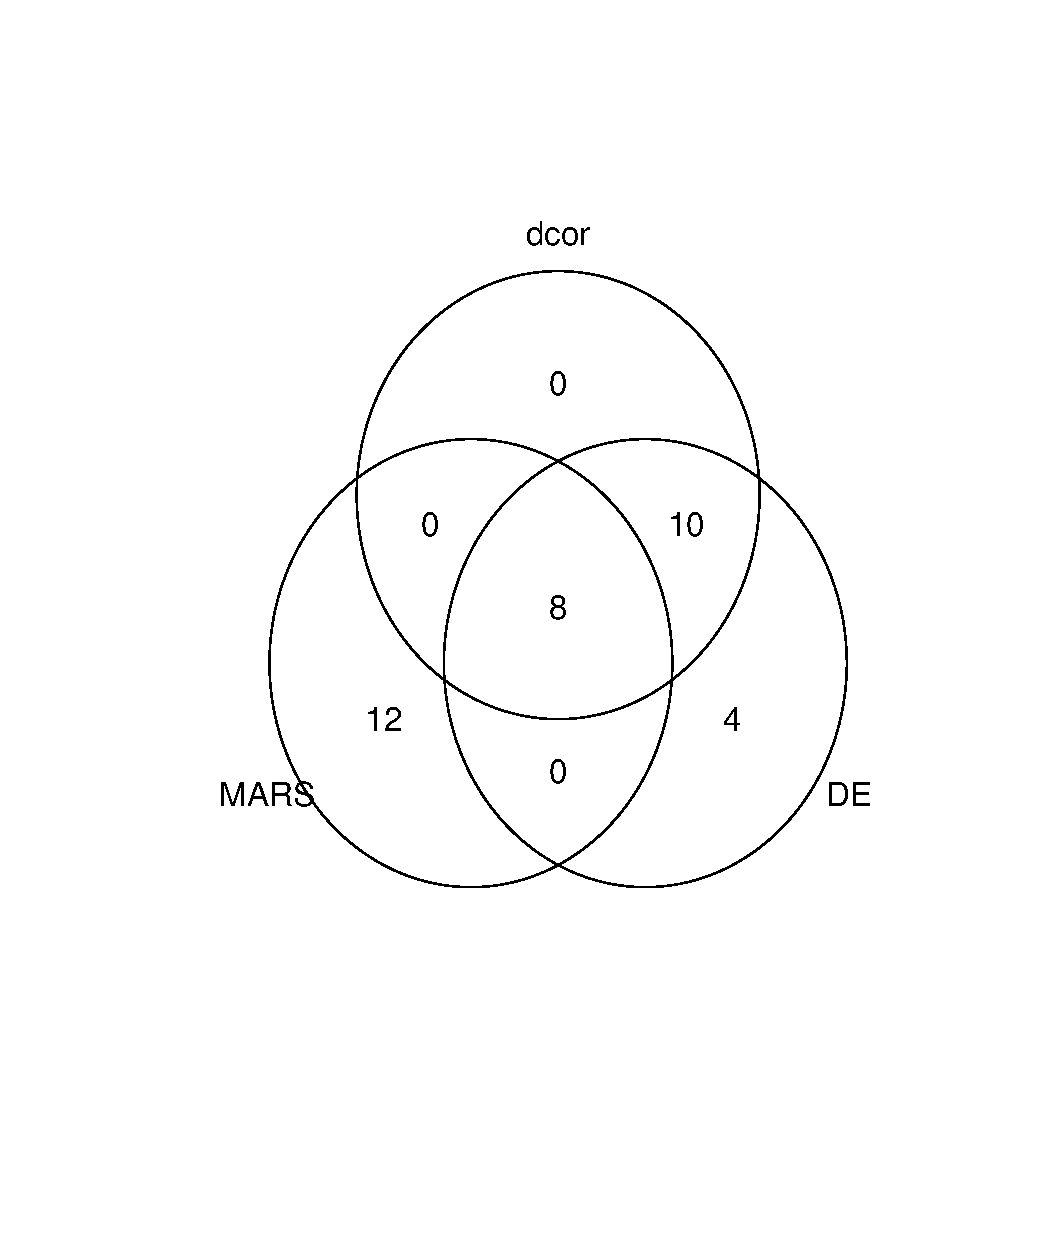
\includegraphics[width=7cm]{vennMARS.pdf}
\caption{Relationship of variables selected by $dcor$ (two-way and three-way), MARS and which were differentially expressed (\gls{DE}).} 
\label{F:vennMARS}
\end{centering}
\end{figure}


\section{Discussion}
There is strong evidence that two-way associations are different in lupus patients and controls. Fifteen genes were identified as having strong two-way associations that were present in lupus patients but not in controls. These were spread across eleven different chromosomes. No strong associations were found in controls that were not also present in lupus patients. Most of these associations are linear in nature and are formed by genes exhibiting the most variability. 

Residual association and non-linear partitioning based methods failed to find any large non-linear associations of interest. The non-linear part of association was between 10\% and 15\% in the two-way associations of interest. The three-way analysis also failed to identify any significant non-linearities based on residual association. Of the three-way associations of interest, the non-linear part of association was again between 10\% and 15\%. The three-way analysis produced many apparent false-positives seemingly arising from the fact that if two variables are strongly associated the extra information provided by a third variable necessarily increases the association.

The two-way analysis suggests that on the lupus dataset $dcor$ identified all associations of interest at the $\ge 0.90$ level.  $dcor$ appears to be biased upwards from $R^2$ (median = 0.16 vs 0.02) but has a high ($\ge 0.8$) concordance with $R^2$ as measured by Kendall's $\tau$. Part of the upward bias can be explained by the fact that $R^2$ was calculated as Pearson's $\rho^2$, so for very strong correlations the corresponding association value is lowered, for example $0.95^2 = 0.9025$. A possible explanation for remainder of the upward bias could be the additional non-linear relationships which $dcor$ can identify but are missed by $R^2$. Both $A$ and $MIC$ failed to identify many linear associations of interest. $A$ is biased upwards from $MIC$, concordance between the two is relatively low ($\tau \approx 0.6$) even at the $\ge0.90$ level.

In the three-way analysis $dcor$ appeared to outperform $A$. The results suggest that $dcor$ is again upward biased from $R^2$. Concordance and agreement between $dcor$ and $R^2$ was lower than in the two-way case. This was more pronounced in controls, so possibly due to the smaller sample size. $A$ failed to identify many three-way linear relationships. Surprisingly the identification rate decreased in lupus patients which had a larger sample size.  

In both the two and three-way cases the GRSq of the associated MARS models showed a small improvement by allowing the explanatory variables to be treated as `hinge' functions, providing further evidence that the main associations were linear but that classification could be improved by allowing non-linearities. Using the full set of variables in the MARS model showed that classification performance was primarily related to the amount of variable interaction permitted rather than whether or not the variables were treated linearly or non-linearly. There was partial overlap between the genes selected by MARS and those by $dcor$. As with other some other data mining methods the chosen variables can be artefacts of the underlying variable selection algorithm and so need to be treated with caution. This is one of the areas where explicit association identification offers distinct advantages.

\chapter{Measuring Association: The Test Data}
This chapter documents the association analysis on the test dataset using the approach developed in Chapter 5. The test dataset consisted of the full Affymetrix biochip described in Section 3.1. As described in Section 3.1 no sample description data was available so only 397 out 1024 observations were identifiable as lupus patients or controls, hence the numbers of controls is very low at only 29 observations.

The heatmap in Figure \ref{F:bigHeat} shows the top 1000 probes showing greatest difference between lupus patients and controls in a $limma$ model. Clustering using $1 - dcor$ was used to order the rows (patients) and columns (probes). The vertical band indicates controls in orange and lupus patients in yellow. Annotation was attempted using Bioconductor (see Section 3.1) but missed many probes meaning that no genetic locations could be added. The plot shows that clusters of controls do form, however there is some overlap lupus patients. Several distinct clusters of probes can be seen suggesting that strong two-way associations exists.

\begin{figure}[h]
\begin{centering}
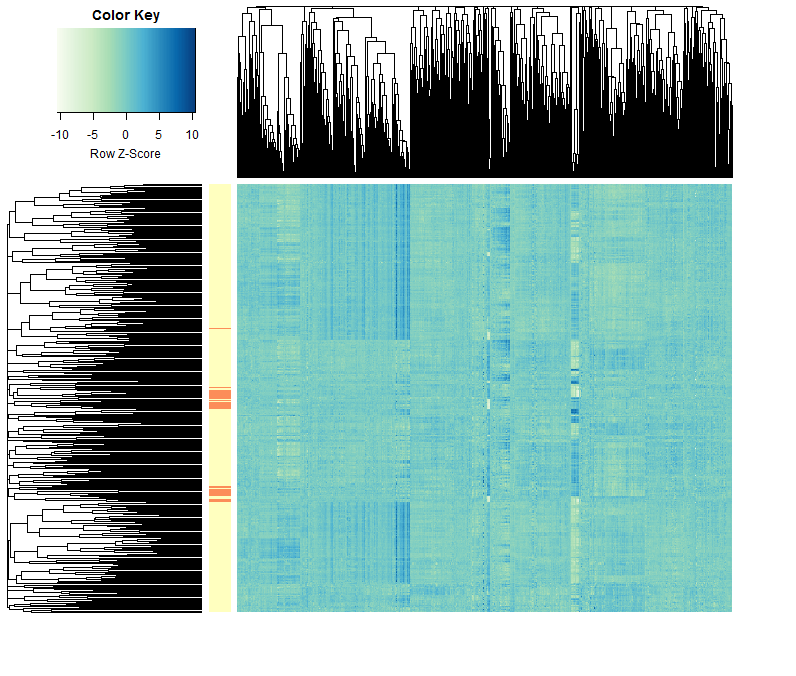
\includegraphics[width=\textwidth]{bigHeatSafe}
\caption{$1-docr$ based heatmap of the top 1000 genes showing greatest difference between lupus patients and controls in a $limma$ model. The row band shows controls in orange and lupus in yellow.} 
\label{F:bigHeat}
\end{centering}
\end{figure}

\section{Methods}
The methods followed that described in Section 5.1. Due to computational limitations the analysis could only be performed on two-way associations. Some modifications to the method used for the two-way association analysis are discussed in the next section.  Differential expression analysis using $limma$ and MARS based classification were also performed.

\subsubsection{Computing}
No large computing infrastructure was available so all of the analysis was conducted on a single laptop (Intel(R) Core(TM) i7-4800MQ CPU @ 2.70GHz) with 16Gb of memory (RAM). Both memory and processing problems were encountered during the analysis.

The test data set consisted of 54,675 probes giving 1494650475 pairs making it a big data problem in that an R matrix for a single association measure exceeded the available memory. %There are a number of R packages which aim to address these problems, such as the $ff$ which presents a `virtualised' interface to the data by keeping a subset of the data in memory while most of the data is stored on disk. 
An additional problem is the processing time required to measure a single two-way association using each measure. Table \ref{T:times} gives the total elapsed time to measure 10000 associations between two vectors of length 320 (320 was taken to be representative of the test data). While they were not recorded under strict control conditions they illustrate that an exhaustive search of all two-way associations could not be performed using the available hardware. The scalability of each implementation could be formally assessed using asymptotic algorithm analysis \cite{knuth} but this was beyond the scope of the project.

\begin{table}[H]
\begin{centering}
\begin{tabular}{cccc}
  \hline
Association & Total Elapsed Time & Associations per second \\ 
  \hline
$R^2$ & 0.57  & 17543.9 \\ 
dcor & 281.94  & 35.5   \\ 
MIC & 448.47  & 22.3   \\ 
A & 1123.57  & 8.9   \\ 
   \hline
\end{tabular}
\caption{Comparison of the times to process 10000 two-way associations of vectors of length 320 on an Intel I7 processor.} 
\label{T:times}
\end{centering}
\end{table}

The processing times meant that only a subset of the possible pairs could be measured using $A$, $MIC$ and $dcor$, however all pairs could be measured using $R^2$. The analysis on the training data demonstrated that $dcor$ had a high concordance with and was upward biased from $R^2$. %The training data set had very low proportions of $R^2$ values $\ge$ 0.7. All of the genes in strong associations were in the top 5\% most variable  genes in the training dataset as measured by both standard deviation and IQR. 
Based on these observed results, $R^2 \le 0.6$ was used as a filter to identify a reduced set of possible pairs which were then measured using the more computationally intensive $dcor$, $A$ and $MIC$. To avoid memory issues, $R^2$ association matrices were incrementally created and searched and the pairs of interest returned.

A risk of this approach is that the search for associations was only partial so potentially interesting associations may have been missed. Larger computing infrastructures could easily handle the workload required for a full evaluation of all associations. However, regardless of the size of the computing resources available, limits will always exists and the filtering approaches adopted could be easily scaled up and lend themselves to parallelisation.


\section{Differential Expression}
All genes were tested for differential expression between lupus patients and controls. Figure \ref{F:BDVolcano} (a) shows a mean-difference plot suggesting that some genes show a large difference between controls and lupus patients. Figure \ref{F:BDVolcano} (b) shows a volcano plot of the FDR adjusted $p$-values. The number of significant results is surprisingly high but only 119 of these had a log fold change $\ge 1$, these are given in Appendix \ref{T:bigDE}. Genes are differentially expressed in both directions, in contrast to the training dataset where all differentially expressed genes were higher in lupus patients than controls. All of the differentially expressed genes from the training data are also differentially expressed in the test data with a log fold change $\ge 1$. No additional genes of biological interest were differentially expressed in the test data. 

\begin{figure}[H]
    \centering
 \subfloat[MA Plot]{{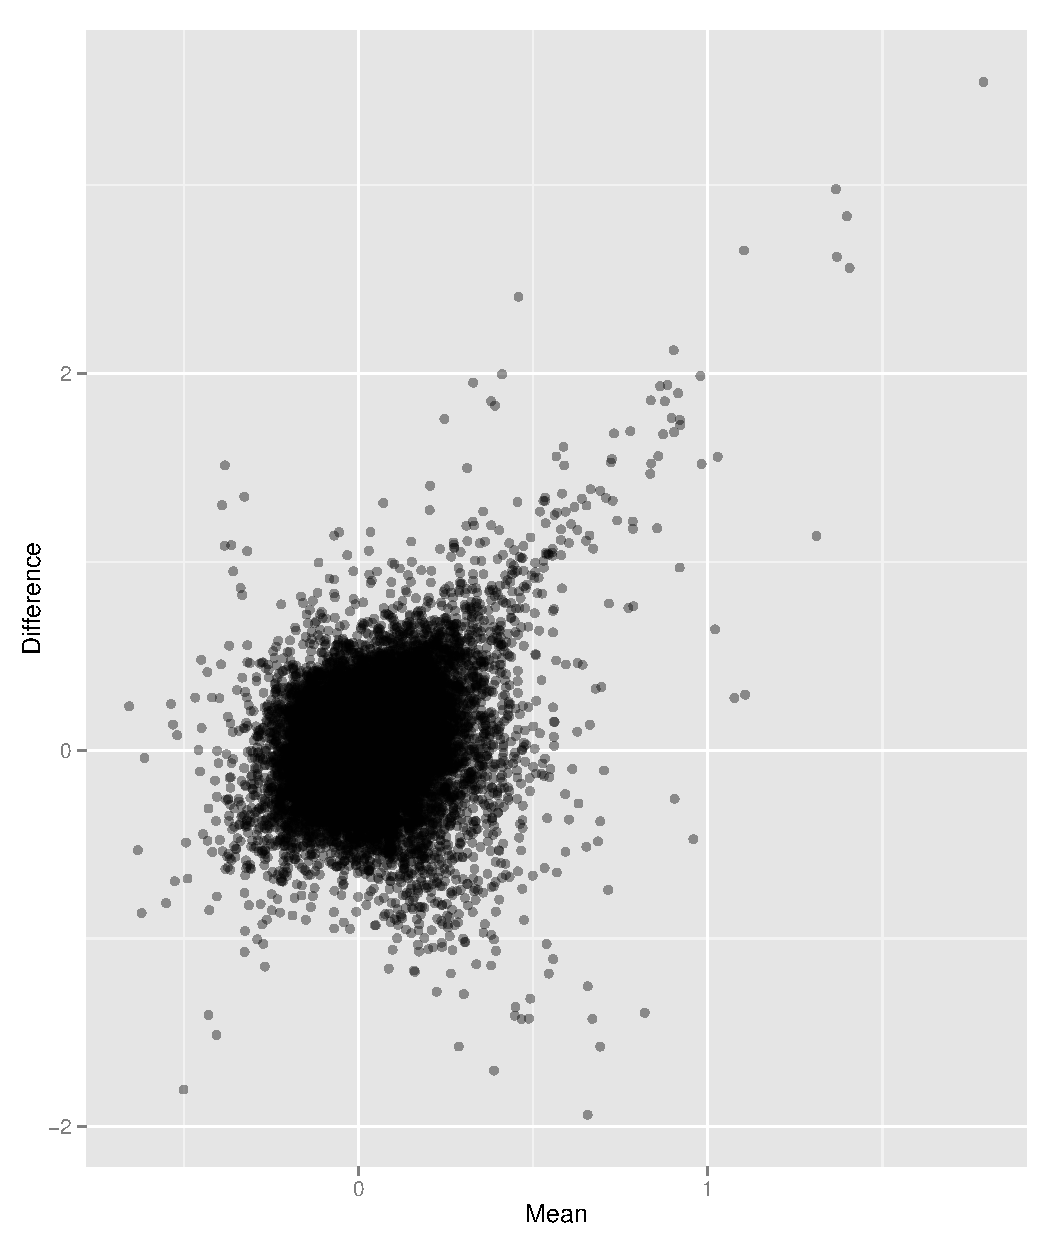
\includegraphics[width=6cm,]{mdbdSafe} }}%
    \qquad    
    \subfloat[Volcano Plot]{{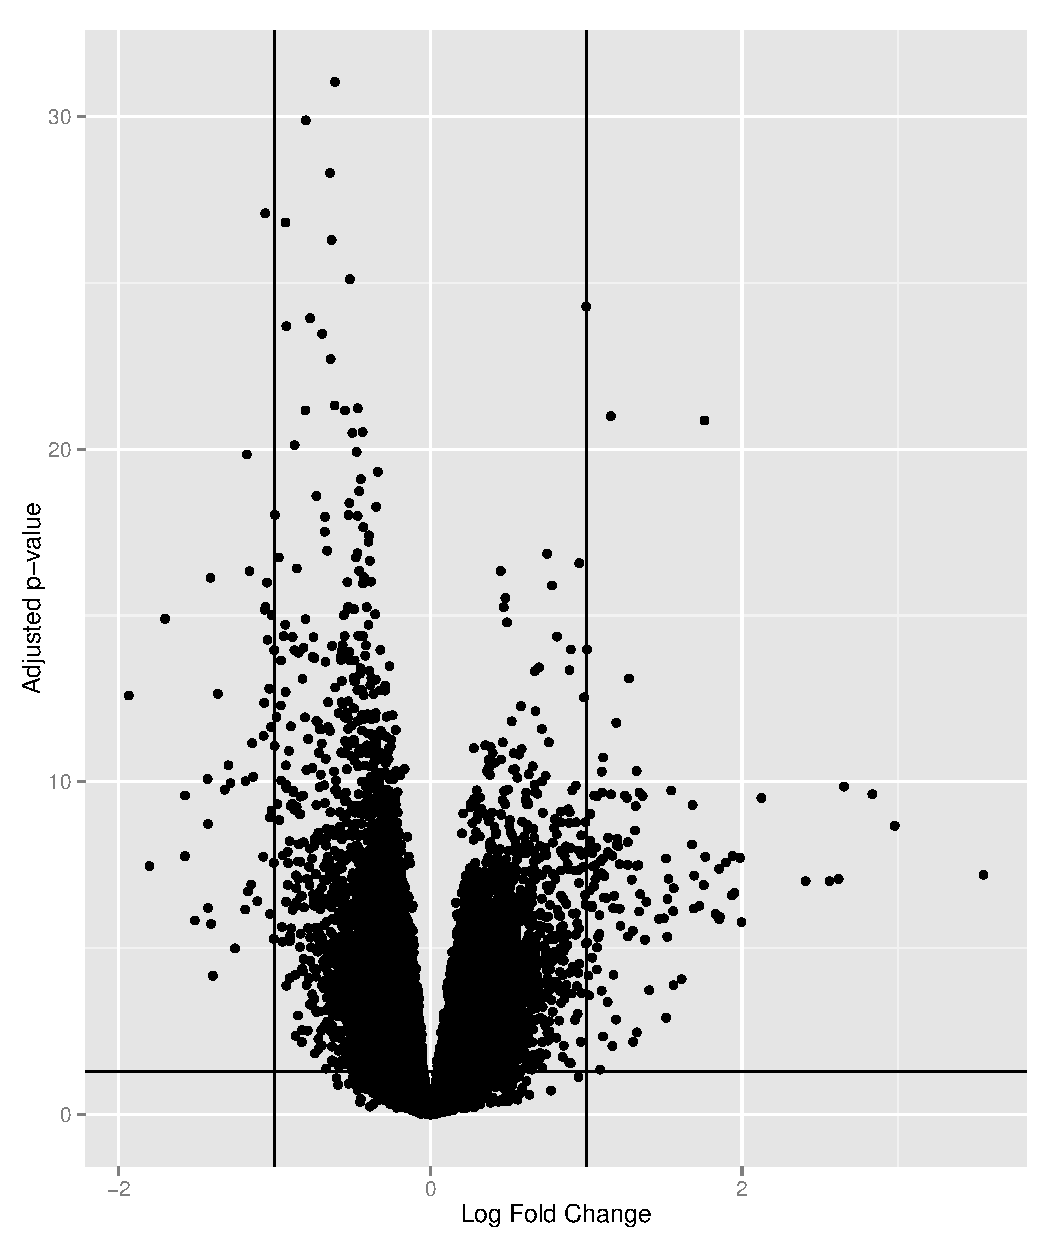
\includegraphics[width=6cm]{volcanoBDSafe.pdf} }}%
    \caption{(a) shows the MA or mean difference plot of lupus patients and controls for the test data. (b) shows a volcano plot showing the results of the $limma$ based differential expression (DE) analysis between lupus patients and controls.}
    \label{F:BDVolcano}
\end{figure}

\section{Two-way Association}
The computational issues described in Section 6.1 meant that the full set of all two-way associations could not be analysed. These results are based on the reduced set:


\[
(X_i, Y_i) = \{\theta_{lupus} \ge \alpha \} \cap \{ (\theta_{control}  \ge \alpha \}
\]

where $X$ and $Y$ are probes, $\theta = R^2$, $i \in {1:54675}$ and $\alpha = 0.6$. The box plot in Figure \ref{F:bigBox} shows that as with the training data two-way associations are higher in controls than lupus patients. The barchart in Figure \ref{F:bigLevels} shows the associations $\ge 0.90$ showing again that $dcor$ many more associations than the other measures. There are also a large number of strong two-way associations in the control group. (Bland-Altman plots comparing each measure of association are provided in Appendix \ref{F:ba2way}.)


\begin{figure}[h]
\begin{centering}
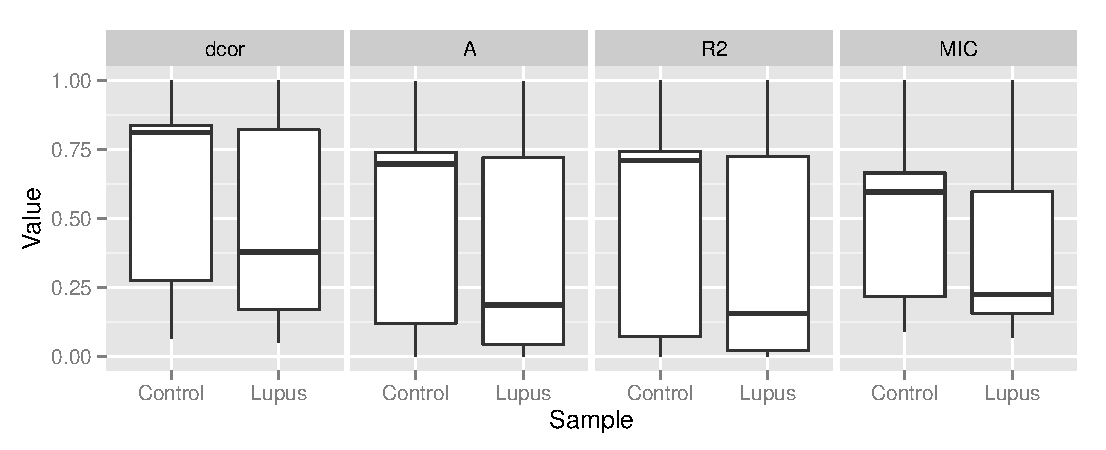
\includegraphics[width=\textwidth]{bigBox.pdf}
\caption{Boxplots of each association measure for controls and lupus patients.} 
\label{F:bigBox}
\end{centering}
\end{figure}




\begin{figure}[h]
\begin{centering}
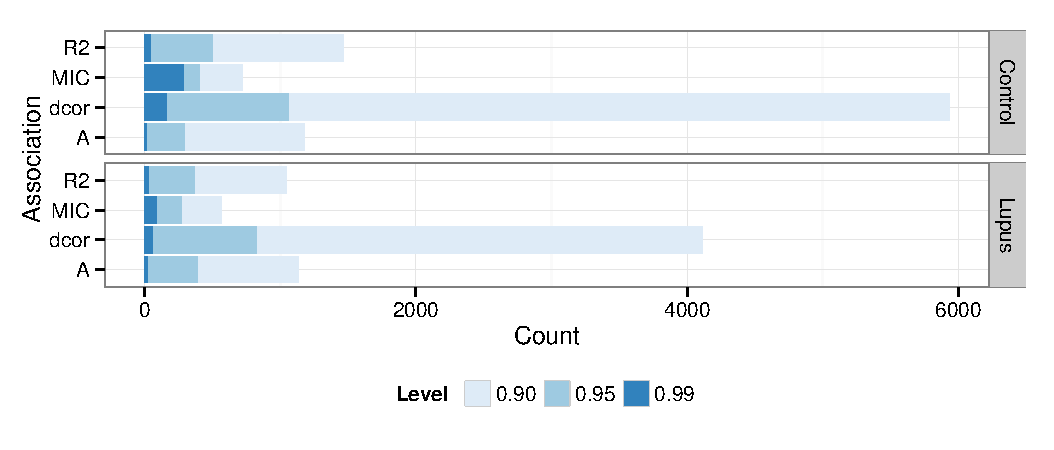
\includegraphics[width=\textwidth]{bigBar.pdf}
\caption{Two-way associations $\ge 0.90$.} 
\label{F:bigLevels}
\end{centering}
\end{figure}


\begin{figure}
    \centering
    \subfloat[Controls]{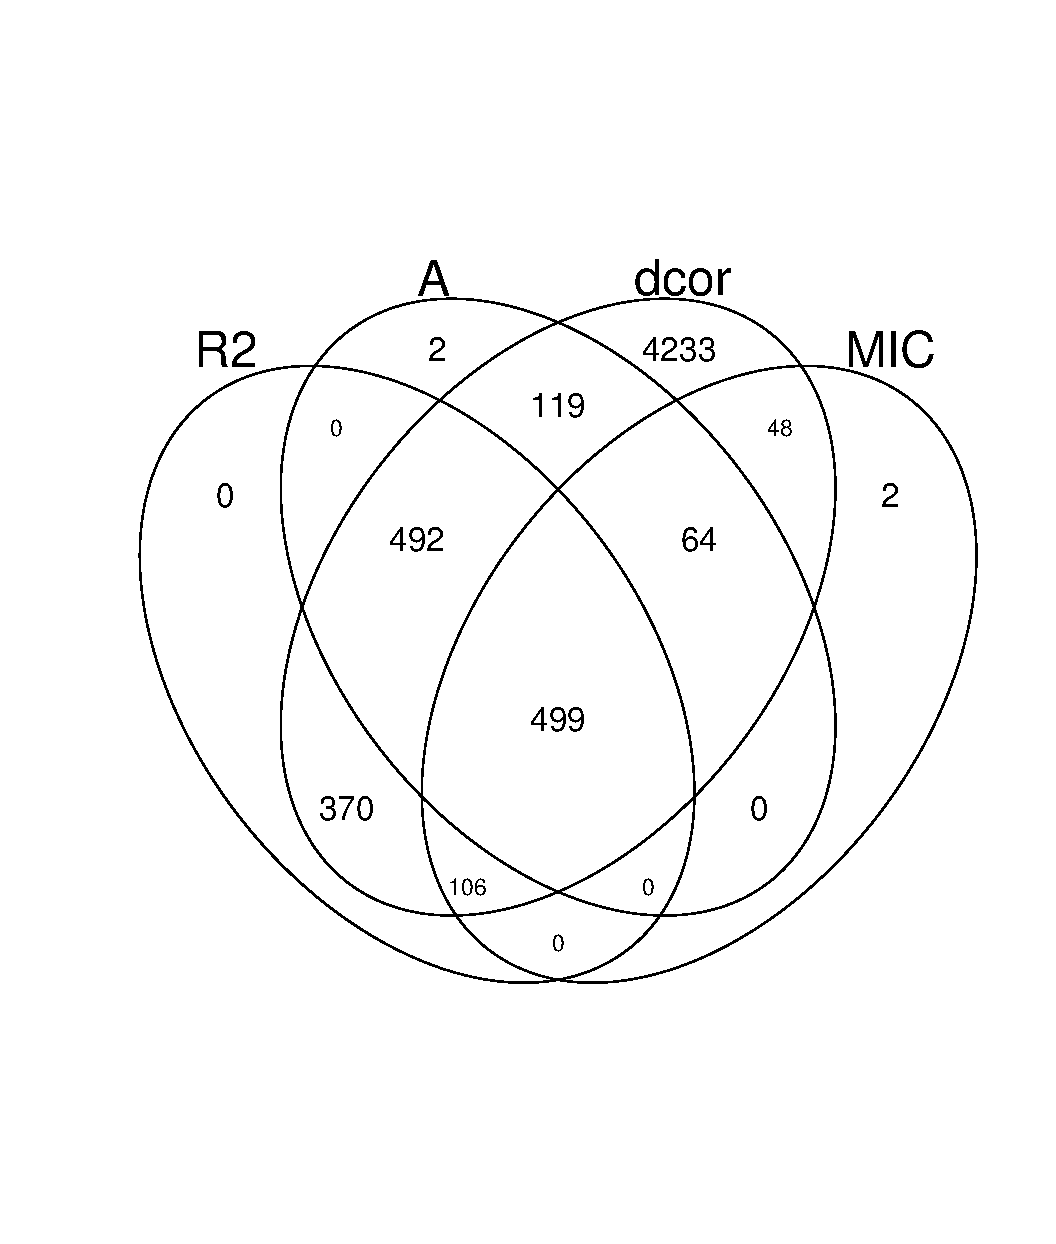
\includegraphics[width=5cm]{bigVenn2C.pdf} }
    \qquad
    \subfloat[Lupus]{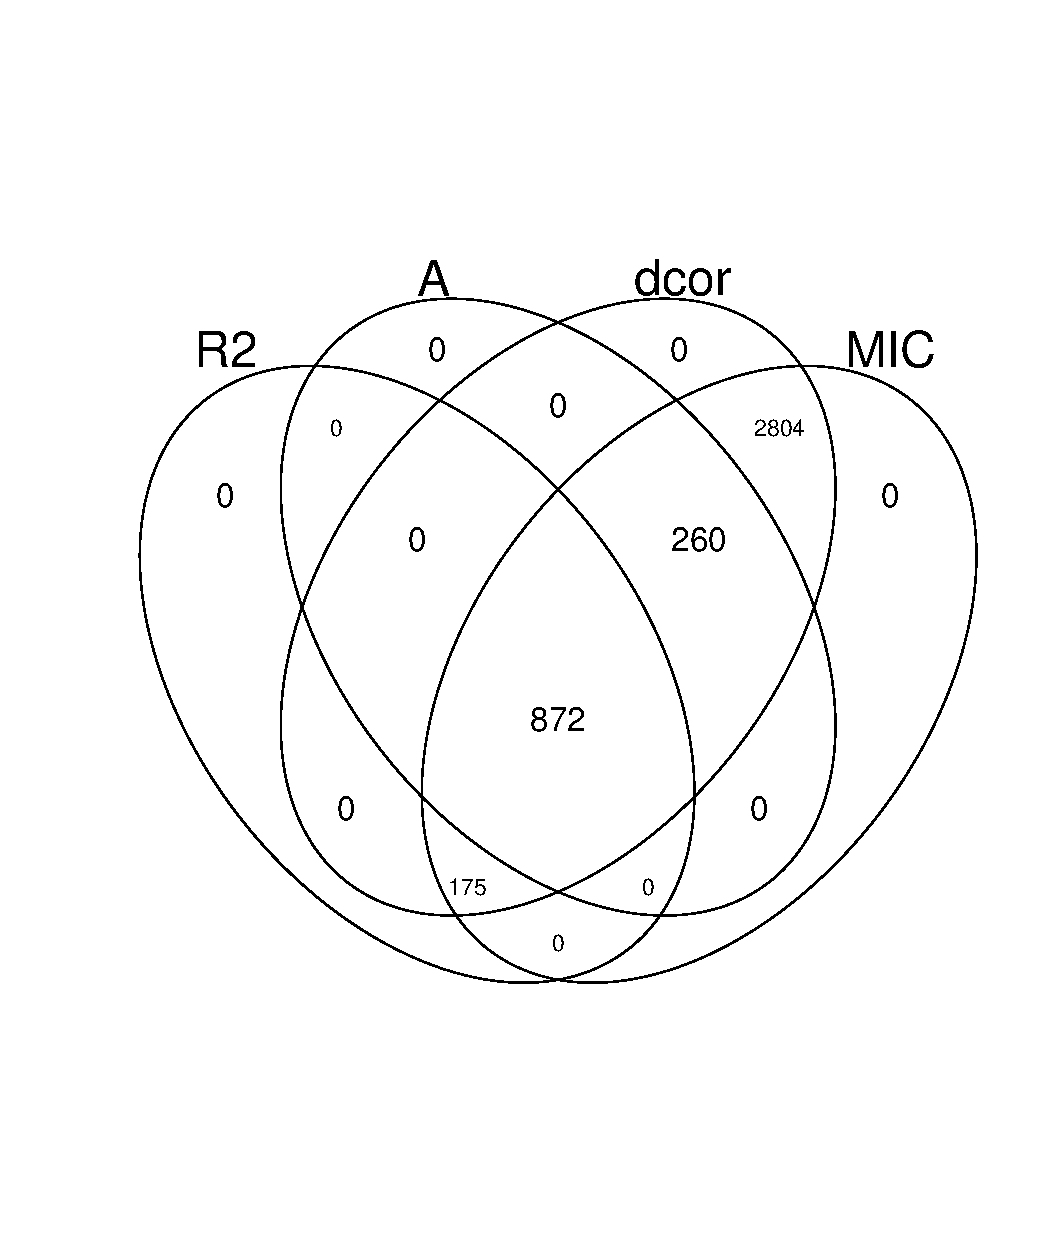
\includegraphics[width=5cm]{bigVenn2L.pdf} }
    \caption{Venn diagrams showing three-way associations $\ge 0.90$.}
    \label{F:VennBig}
\end{figure}

Figure \ref{F:VennBig} compares each measure showing that $dcor$ identifies almost all associations identified by $A$ and $MIC$. Of the four associations in the control group identified by A and MIC but missed by $dcor$, all had $dcor$ values of 0.88 and 0.89 so are just an artefact of the threshold applied rather than interesting associations missed by $dcor$. 

The analysis found 57 pairs showing large differences between lupus patients and controls. These involved 53 genes, 38 of which were differentially expressed.  Scatterplots of the top sixteen results for lupus patients are shown in Figure \ref{F:bigScatter}, again loess was used to fit smoothed lines to the data. The plots show some evidence of quadratic relationships. The non-linear part of association was again between 10\% and 15\%.  None of the associations of interest from the training dataset matched those in the test dataset. The reason for this was that in the test dataset these relationships had very strong linear associations ($R^2$ between 0.87 and 0.91) so the non-linear part of association was correspondingly low (between 3\% and 4\%). Bootstrap estimates of association for these pairs are provided in Appendix \ref{T:bigAE}.

The analysis also found 770 associations in controls that differed from lupus patients. These involved 397 genes only 9 of which were differentially expressed. Visual examination suggested that some of these genes had bimodal distributions and that the results may be false positives arising from the very small control sample sizes. The frequency of the probes involved in these associations is shown in Figure \ref{F:bigFilter}. The x-axis is ordered by the log fold change in gene expression levels as measured by $limma$. The upper plot shows that most of the two-way associations in lupus patients are also strongly expressed. In the case of controls the frequencies are more evenly distributed.

\begin{figure}[H]
\begin{center}
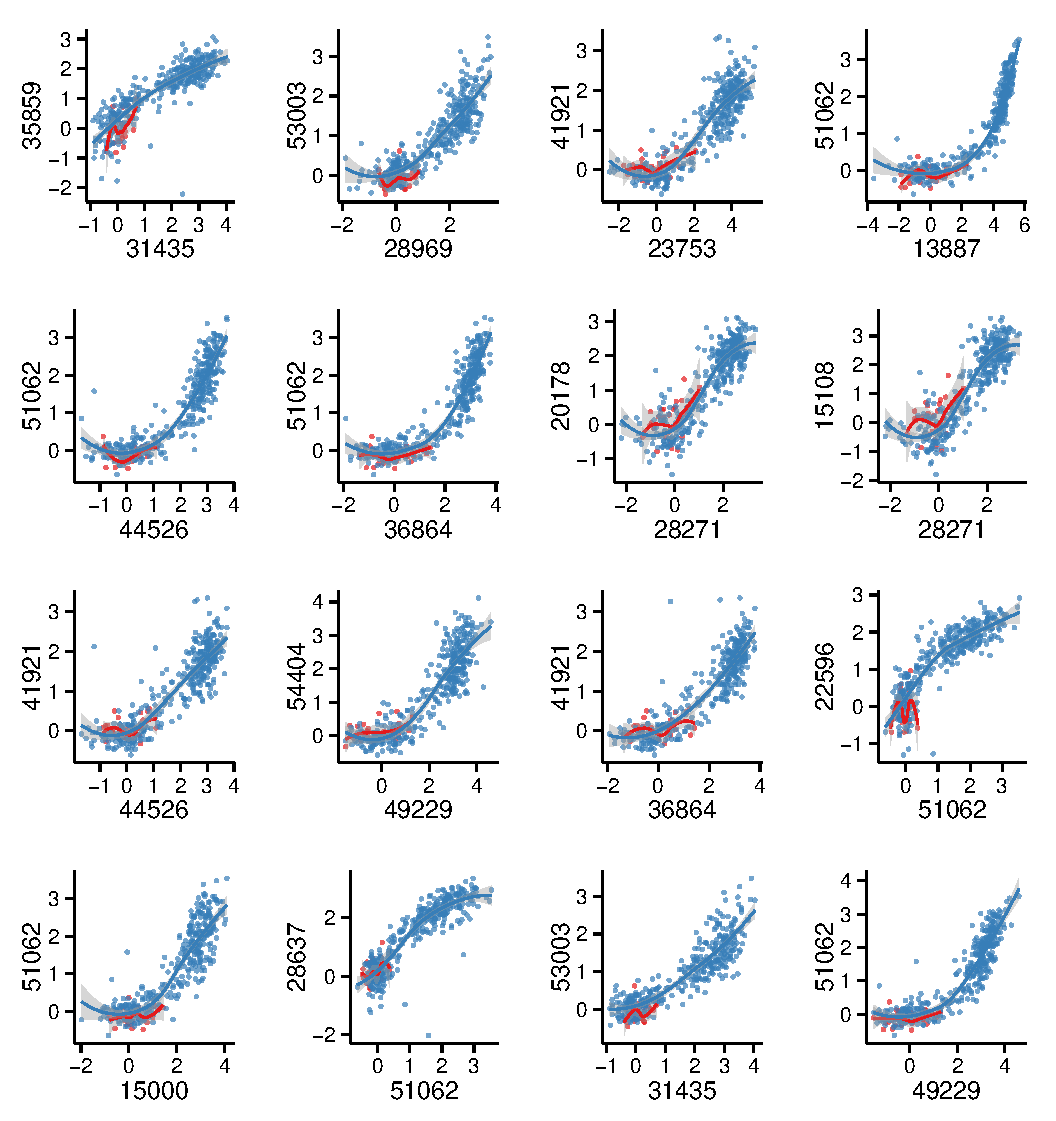
\includegraphics[width=\textwidth]{bigScatter}
\caption{The top16 two-way associations $\ge 0.90$ that differ between lupus patients and controls.} 
\label{F:bigScatter}
\end{center}
\end{figure}


\begin{figure}[H]
\begin{centering}
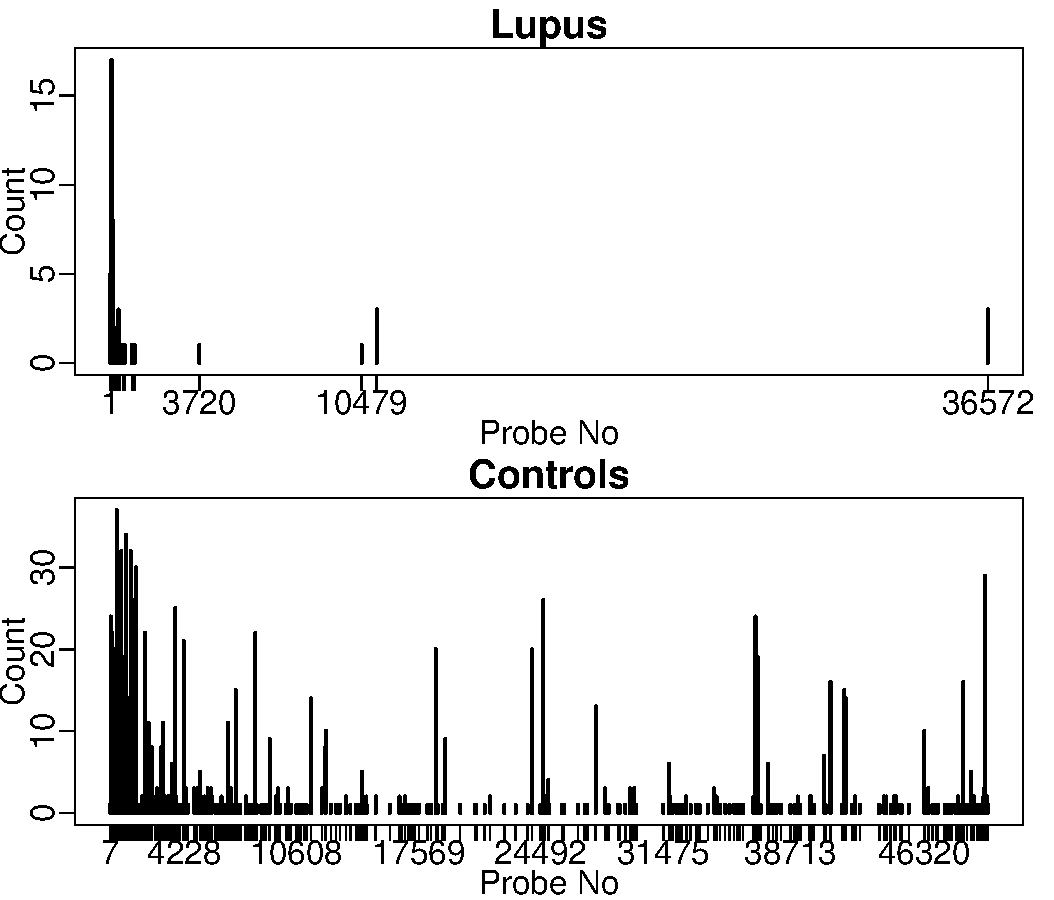
\includegraphics[width=12cm]{bigFilterSafe.pdf}
\caption{Frequency of probes involved in two-way associations in lupus patients and controls.} 
\label{F:bigFilter}
\end{centering}
\end{figure}

\section{MARS}
The same combination of MARS models were fit as described in Section 5.4. A 70:30 train:test split was again used, so all probes could be input as explanatory variables. All models showed very high classification results as measured by the ROC AUC, the ROCs are shown in Figure \ref{F:bigROC}. Treating the explanatory variables linearly moderately improved classification performance. Allowing variable interactions had only a minor effect on the results.

The results again need to be treated with caution due to the low numbers of controls (29) relative to lupus patients (367), for example if a classifier predicted that a sample was a lupus patient every time the classification rate would still be $\approx 0.93$. 

The most important variables as selected by MARS were 35160\_at, AFFX-DapX-3\_at, AFFX-r2-Bs-dap-3\_at, 226827\_at, 213855\_s\_at, 1558756\_at, 226842\_at, 201432\_at, 230737\_s\_at. Two of these (AFFX-DapX-3\_at, AFFX-r2-Bs-dap-3) were differentially expressed but none were identified in the two-way association analysis. A possible explanation for this is the fact that each analysis has different objectives but that all of the results may be sensitive to the low sample sizes used. Another factor is the sensitivity of MARS' variable selection procedure to collinear datasets.

\begin{figure}[H]
\begin{centering}
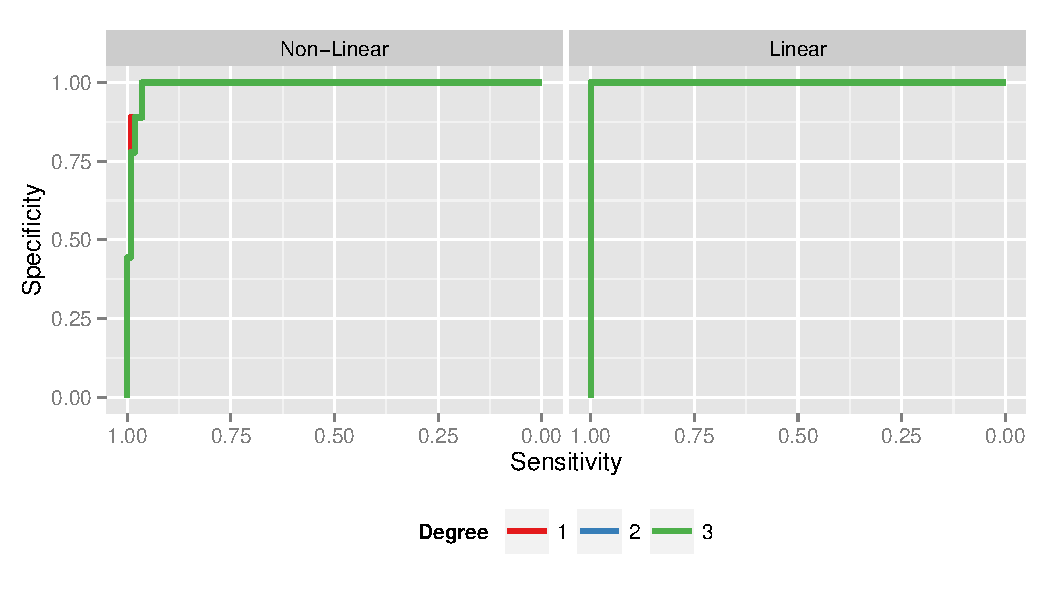
\includegraphics[width=12cm]{bigROC}
\caption{Frequency of probes involved in two-way associations in lupus patients and controls.} 
\label{F:bigROC}
\end{centering}
\end{figure}


\section{Discussion}
$dcor$ again outperformed both $A$ and $MIC$ in terms of associations identified. Of the associations identified the difference from the training dataset is explained by reduced non-linear part of association for these pairs in the test set. No strong non-linear associations were found but the non-linear part of association was comparable to that of the training data. The MARS results showed very high classification results in all cases.

The analysis presented in this chapter showed how association analysis can be used in high dimensional datasets where the number of parameters, $p >> n$, the number of observations. The fact that all of the samples in the test dataset could not be identified meant that the sample size for controls was extremely small at only 29 observations. The net effect of this is that the actual results, in terms of gene associations identified, need to be treated with extreme caution. The more important point is that the methods used can be applied to analyse associations in large biological datasets. 

\chapter{Discussion and Further Work}
The goal of the analysis was two-fold: to compare differences in non-linear associations between lupus patients and controls and to compare different measures of association themselves. 

The analysis identified a number of two-way and three-way gene associations of interest that appeared to differ between lupus patients and controls. These associations were primarily linear and only had a small (10\% to 15\%) non-linear part of association. Most of the genes forming strong associations were also differentially expressed between lupus patient and controls. Association analyses are essentially exploratory in nature and provide no evidence of causation. There are numerous sources of technical and biological variation which might be responsible for observed associations. In reality the results of an association analysis would serve as the basis for a more refined follow on study or, if the goal is to establish causality, a suitably designed controlled experiment. 

Of the measures of association studied, on balance, $dcor$ had better performance than either $A$ or $MIC$ on the lupus data in terms of associations identified. The simulations suggest that $dcor$ generally has greater power with small sample sizes and noisy datasets but that $MIC$ and $A$ have greater power for certain functional types. Knowing the relative strengths and weaknesses of each measure is a critical aspect to choosing which association to use. The  choice of which to use might depend on the types of functional relationships suspected to exist in the data or to the extent of the computational resources available. A pragmatic option is to combine a number of measures such as $dcor$ and $A$ and use the knowledge of the measures' properties to critically evaluate the results obtained.

There are many other measures of association that could be compared, most notably mutual  information and the Heller-Heller-Gorfine \cite{HHG} measure. Another extension would be to investigate partial associations, i.e. measuring the strength of association while one variable is controlled for. There also a number of alternative methods that can be used to assess inter-variable association and whether or not it can be best described linearly or non-linearly. Two Bayesian approaches to this are an R package called $spikeSlabGAM$ \cite{spikeSlabGAM} and another approach presented by \citet{BayesianGRN} which would make an interesting comparison in a future study. 

The analysis sought to explore non-linear relationships in big data. The focus was on statistical methods which could be scaled given larger computing resources. The limitations of the available computers meant that exhaustive searches of two-way and three-way associations could not be performed on the test data meaning that there is a risk that some associations of interest may have been missed. However the methods used could easily be adapted to a larger computing infrastructure.

The lack of context information about the test dataset was a distinct problem due to the resulting low sample sizes. A particular concern here is the lack of power which the different association measures have in low samples as indicated by the simulations in Chapter 3. Given a complete set of identified samples, the analysis reported in Chapter 6 could be repeated exactly but the increased sample sizes would give greater confidence in the results.

The exploratory data analysis indicated that there were some differences between the different lupus sources. A potential extension would be to explore if systematic differences in gene associations exist between these sources. The main reason for not pursuing this during study was the relatively samples sizes which result from grouping into sources. An added concern was the potential issue of batch effects which could be related to different sources. Batch effects can manifest if gene expression levels on different samples have been measured separately leading to technical variability. While there are many statistical approaches for identifying and trying to handle batch effects should they exist, exploring these issues was beyond the scope of this study.

The analysis would  be enriched by considering additional factors about the samples from which gene expression levels were measured. For example, indicating if there was a potentially interesting biological differences such as sex or age. The genes in the training dataset were annotated with chromosomal information in order to provide evidence against any observed associations of interest just being a side effect of co-expression of proximal genes. A natural extension to this would be to consider associations within gene hierarchies which are thought to have similar biological function such as gene sets or gene regulatory networks. The $limma$ package can incorporate such hierarchical information, so the analysis could be extended accordingly. Another potentially interesting technique to model this is called Gene Set Analysis \cite{efron2007}.

Possible extensions to the simulation were discussed in Section 3.4. A further extension would be to study the sensitivity of both $A$ and $dcor$ to their respective tuning parameters. The bootstrap estimates of both $MIC$ and $A$ appeared to converge more closely with $dcor$ than their point estimates. This could also be studied through simulation however even if the accuracy improves, the added computational overhead might render it impractical.

A refinement to the classification analysis would be to consider misclassification costs. Not all classification errors are equal, misclassifying a lupus patient as a control is likely to more costly than misclassifying a control as a lupus patient. Quantifying such a cost would enable better evaluation of classification performance. MARS was only one of many classification models which could have been chosen. A further advancement would be compare the performance of different model types.

Comparing the results of the association analysis, classification analysis and differential expression analysis is not straight forward as they each have different objectives. When considered in terms of gene involvement the results did show some overlap  but also differences. Many of these differences were a consequence of the somewhat arbitrary thresholds set for what constituted a strong association or a differentially expressed gene. The goal here was to illustrate a general approach that could be tailored to specific needs. In reality such thresholds of evidence are likely to be context specific but general results might still by improved by involving domain expertise to attempt to quantify biologically meaningful levels.

\bibliographystyle{unsrtnat}
\bibliography{refdatabase}

\printglossary

\appendix

\chapter{Simulation Code and Results}

\section{Simulation Code}
The R code for for running the simulations based on that of \citet{Tibshirani2011}.
\lstset{ %
language=R,                % choose the language of the code
basicstyle=\footnotesize,       % the size of the fonts that are used for the code
numbers=left,                   % where to put the line-numbers
numberstyle=\footnotesize,      % the size of the fonts that are used for the line-numbers
stepnumber=1,                   % the step between two line-numbers. If it is 1 each line will be numbered
numbersep=5pt,                  % how far the line-numbers are from the code
showspaces=false,               % show spaces adding particular underscores
showstringspaces=false,         % underline spaces within strings
showtabs=false,                 % show tabs within strings adding particular underscores
frame=single,           % adds a frame around the code
tabsize=2,          % sets default tabsize to 2 spaces
captionpos=b,           % sets the caption-position to bottom
breaklines=true,        % sets automatic line breaking
breakatwhitespace=false,    % sets if automatic breaks should only happen at whitespace
escapeinside={\%*}{*)}          % if you want to add a comment within your code
}
\begin{lstlisting}[
    basicstyle=\tiny, %or \small or \footnotesize etc.
]
#' The null hypothesis. Generates indepenent random variables and measures the association.
#'
#' @param type The type of functional relationship, e.g. linear.
#' @param measures A list of estimates of association.
#' @param distribution The distribution to sample from.
#' @param n The sample size.
#' @param noise The total level of noise.
#' @param noiseLevel The fraction of noise.
#' @param numNoise The noise increment.
h0 <- function(type, measures, distribution, n, noise, noiseLevel, numNoise) {
  y <- type(distribution(n), noise, noiseLevel, numNoise, n)
  x <- distribution(n)
  sapply(measures, function(f) f(x,y))
}

hA <- function(type, measures, distribution, n, noise, noiseLevel, numNoise) {
  x <- distribution(n)
  y <- type(x, noise, noiseLevel, numNoise, n)
  sapply(measures, function(f) f(x,y))
}

#' Simulates a hypothesis nsim times.
#'
#' @param type The type of functional relationship, e.g. linear.
#' @param h h0 or hA
#' @param measures A list of estimates of association.
#' @param distribution The distribution to sample from.
#' @param n The sample size.
#' @param noise The total level of noise.
#' @param noiseLevel The fraction of noise.
#' @param numNoise The noise increment.
simulateTwoWay <- function(type, h, measures, nsim, distribution, n, noise, noiseLevel, numNoise) {
  res <- replicate(nsim, h(type, measures, distribution, n, noise, noiseLevel, numNoise))
  t(res)
}

#' Estimates the power for a functional relationship for the given measures.
#'
#' @param type The functional relationship, e.g. sineLow
#' @param measures The estimates of association, e.g. dcor.
#' @param measureNames The corresponding names.
#' @param nsim The number of times the simulation is repeated.
#' @param distribution The samoling distribution, e.g. runif if ~U, rbeta with relevant parameters 
#'  for a skewed case. 
#' @param noise The total level of noise simulated, e.g. 3.
#' @param noiseLevel The noise level to use.
#' @param numNoise The number of noise levels simulated, e.g. 30. 
#' @return The power estimate for each measure.
powerForType <- function(type, measures, measureNames, nsim, distribution, n, noise, noiseLevel, numNoise) {
  cat("powerForType: n =", n, "noiseLevel =", noiseLevel, "at", format(Sys.time()), "\n")
  hoRes <- simulateTwoWay(type, h0, measures, nsim, distribution, n, noise, noiseLevel, numNoise)
  means <- colMeans(hoRes)
  cuts <- apply(hoRes, 2, quantile, (1 - 0.05))
  haRes <- simulateTwoWay(type, hA, measures, nsim, distribution, n, noise, noiseLevel, numNoise)
  means <- colMeans(haRes)
  powerRes <- colSums(sweep(haRes, 2, cuts, ">"))/nsim
  names(powerRes) <- measureNames
  cat(".")
  powerRes
}

#' Estimates the power of measures of association to detect different types of functional relationships.
#'
#' @param types The bivariate function names.
#' @param measures The functions to estimate association, e.g. dcor.
#' @param measureNamess The corresponding names.
#' @param nsim The number of times the simulation is repeated.
#' @param distribution The samoling distribution, e.g. runif if ~U, rbeta with relevant parameters 
#'  for a skewed case. Use ... for extra paramters.
#' @param noise The total level of noise simulated, e.g. 3.
#' @param noiseLevels The number of noise levels simulated, e.g. 1:30.
#' @param sizes The smaple sizes to use, e.g. c(50, 100, 250, 500)
#' @param ncores The number of cores to use for processing. Use "all" for maximum available.
#' @return A tidy dataframe with the results.
#' 
estimatePower <- function(types, measures, measureNames, nsim, distribution, noise, noiseLevels, sizes, ncores='all') {
  #build a grid of all noise levels and sample sizes
  parameters <- expand.grid(sizes, noiseLevels)
  colnames(parameters) <- c("n", "noiseLevel")
  
  powerNoiseAndSize <- function(fn) {
    cat("Simulating ", fn, "at", format(Sys.time()), "\n")
    f <- match.fun(fn)   
    res <- apply(parameters, 1, function(x) powerForType(f, measures, measureNames, nsim, distribution, x[1], noise, x[2], max(noiseLevels)))
    res <- data.frame(t(res))
    res <- cbind(res, parameters)
    res$Function <- fn
    res
  }
  
  #use a sensible number of cores for processing
  if (ncores == 'all') {
    ncores <- detectCores() -1
    if (length(types) < ncores) {
      ncores <- length(types)
    }
  }

 # do the work in parallel
  sfInit( parallel=TRUE, cpus=ncores, slaveOutfile='logs/log.txt')
  sfLibrary(nlf)
  sfLibrary(energy)
  sfLibrary(matie)
  sfLibrary(minerva)
  sfExportAll()
  #sfExport('powerForType', 'simulateTwoWay', 'h0', 'hA', 'parameters', 'measures', 'measureNames', 'noise', 'r2', 'spear')
  res <- sfLapply(types, powerNoiseAndSize)
  sfStop()
  
  #format the results
  res <- plyr::ldply(res)
  gather(res, key = measure, value = power, -n, -Function, -noiseLevel)
}

#script to run the power simulation

#get all function types from the nlf package
types <- ls(getNamespace("nlf"), all.names=F)

#define the association measures to use
measures <- c(r2, spear, dcor, myMA, myMine)
measureNames <- c('A', 'MIC')
sizes=c(10,20,30,40,50,75,100,125,150,200,250,300,350,400,500,750,1000)

#run the simulation for the ~Uniform case
system.time(res <- estimatePower(types, 
                                 measures, 
                                 measureNames, 
                                 nsim=500, 
                                 runif, 
                                 noise=3, 
                                 noiseLevels = 1:30, 
                                 sizes=sizes))
res$Distribution <- "Uniform"


#2D scatter plots of power vs noise for all associations and function types
ggplot(res, aes(noiseLevel, power, colour=measure)) +
  geom_line(size=1.1) +
  facet_grid(n~Function)+
  theme(legend.position="bottom")

\end{lstlisting}

\section{Simulation Results}

\begin{figure}[H]
\begin{centering}
\includegraphics[width=\textwidth]{forms.pdf}
\caption{Scatter plots showing the fifteen different functional forms with varying amounts of random noise. In each plot the darkest points show the minimum noise added while the lighter points show increasing levels of noise. The differences in the y-axes reflect the differences in the range of $y$ for each function.} 
\label{F:FunctionFormsNoise}
\end{centering}
\end{figure}

\begin{figure}[H]
\begin{centering}
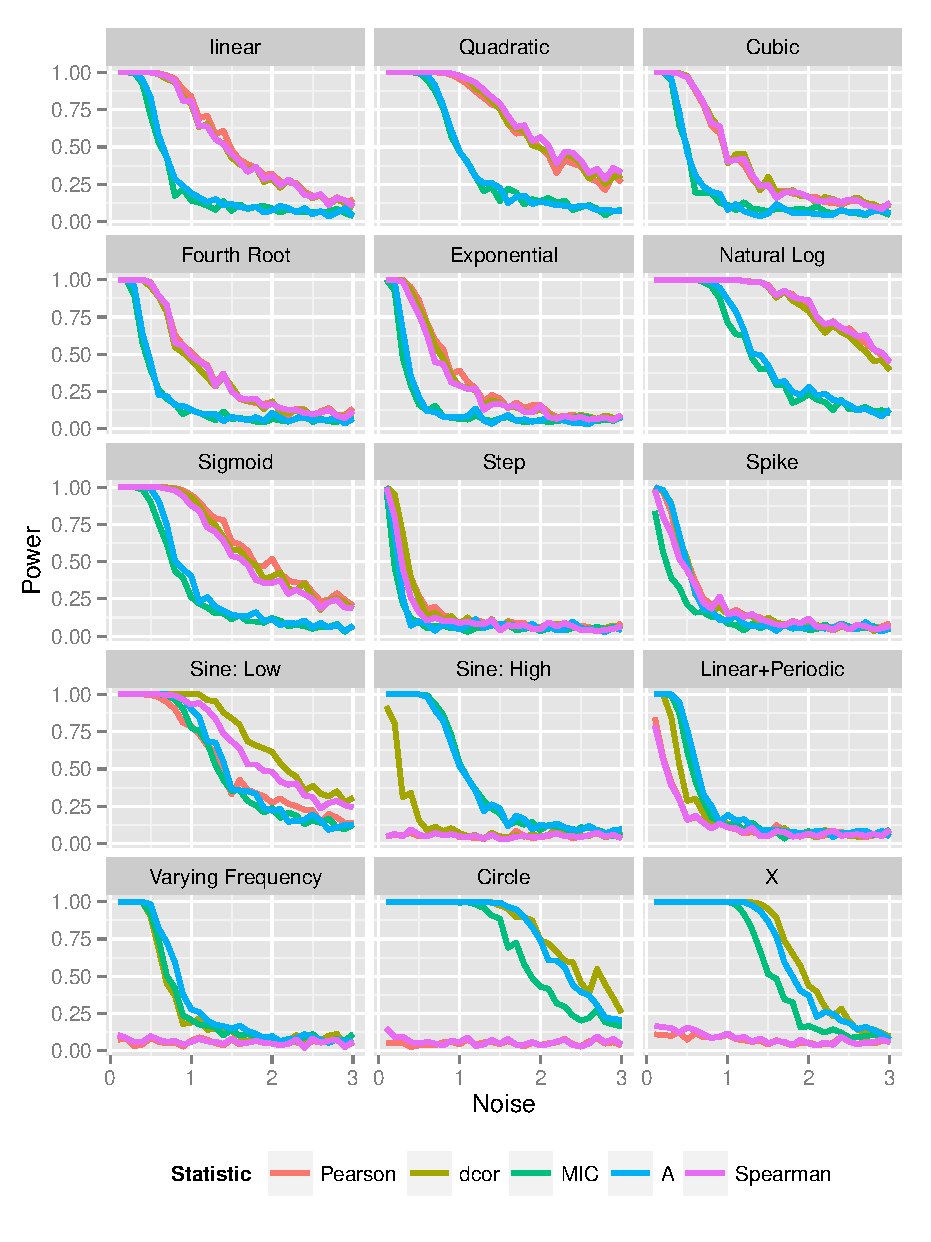
\includegraphics[width=\textwidth]{beta25Noise.pdf}
\caption{Scatter plots showing the power of each measure of association vs. noise for each functional form based on 320 observations from a $Beta(2,5)$ distribution. Note the reduction in power for the step function.} 
\label{F:powerNB}
\end{centering}
\end{figure}



\begin{figure}[H]
\begin{center}
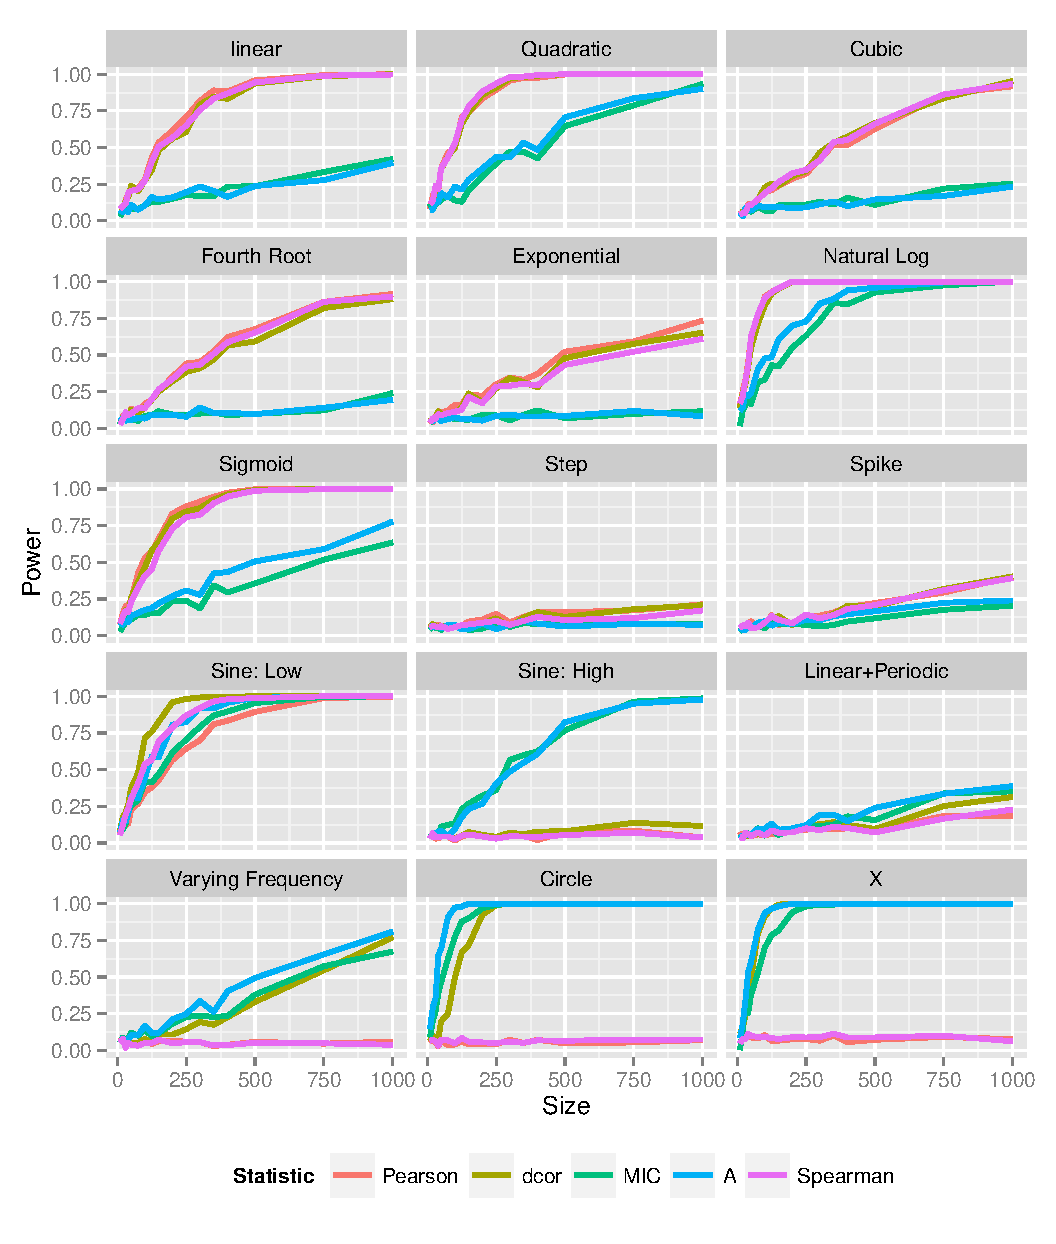
\includegraphics[width=\textwidth]{powerSizeBeta25Noise10Final.pdf}
\caption{Scatter plots showing the power of each measure of association vs. size for each functional form based on a $Beta(2,5)$ distribution. For the exponential function the power reduced for $dcor$, $A$ and $MIC$.} 
\label{F:powerSB}
\end{center}
\end{figure}

\begin{figure}[H]
\begin{centering}
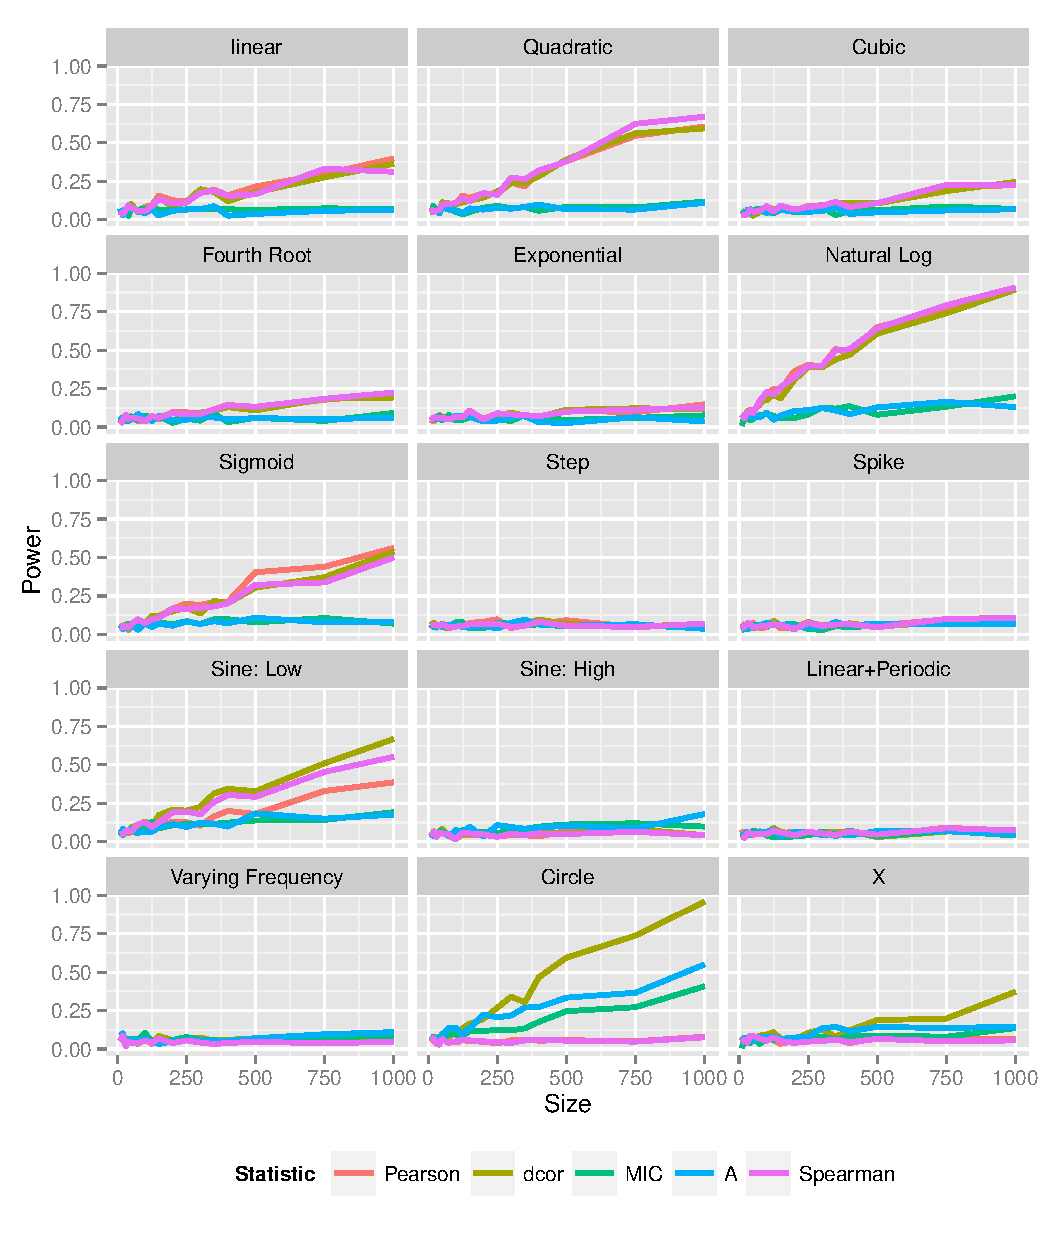
\includegraphics[width=\textwidth]{powerSizeNoise30Beta25.pdf}
\caption{Scatter plots showing the power of each measure of association vs. sample size for each functional forms. None of the measures converged.} 
\label{F:powerSizeBN30}
\end{centering}
\end{figure}



%\chapter{Additional Exploratory Methods}
%
%\begin{figure}[h]
%\begin{center}
%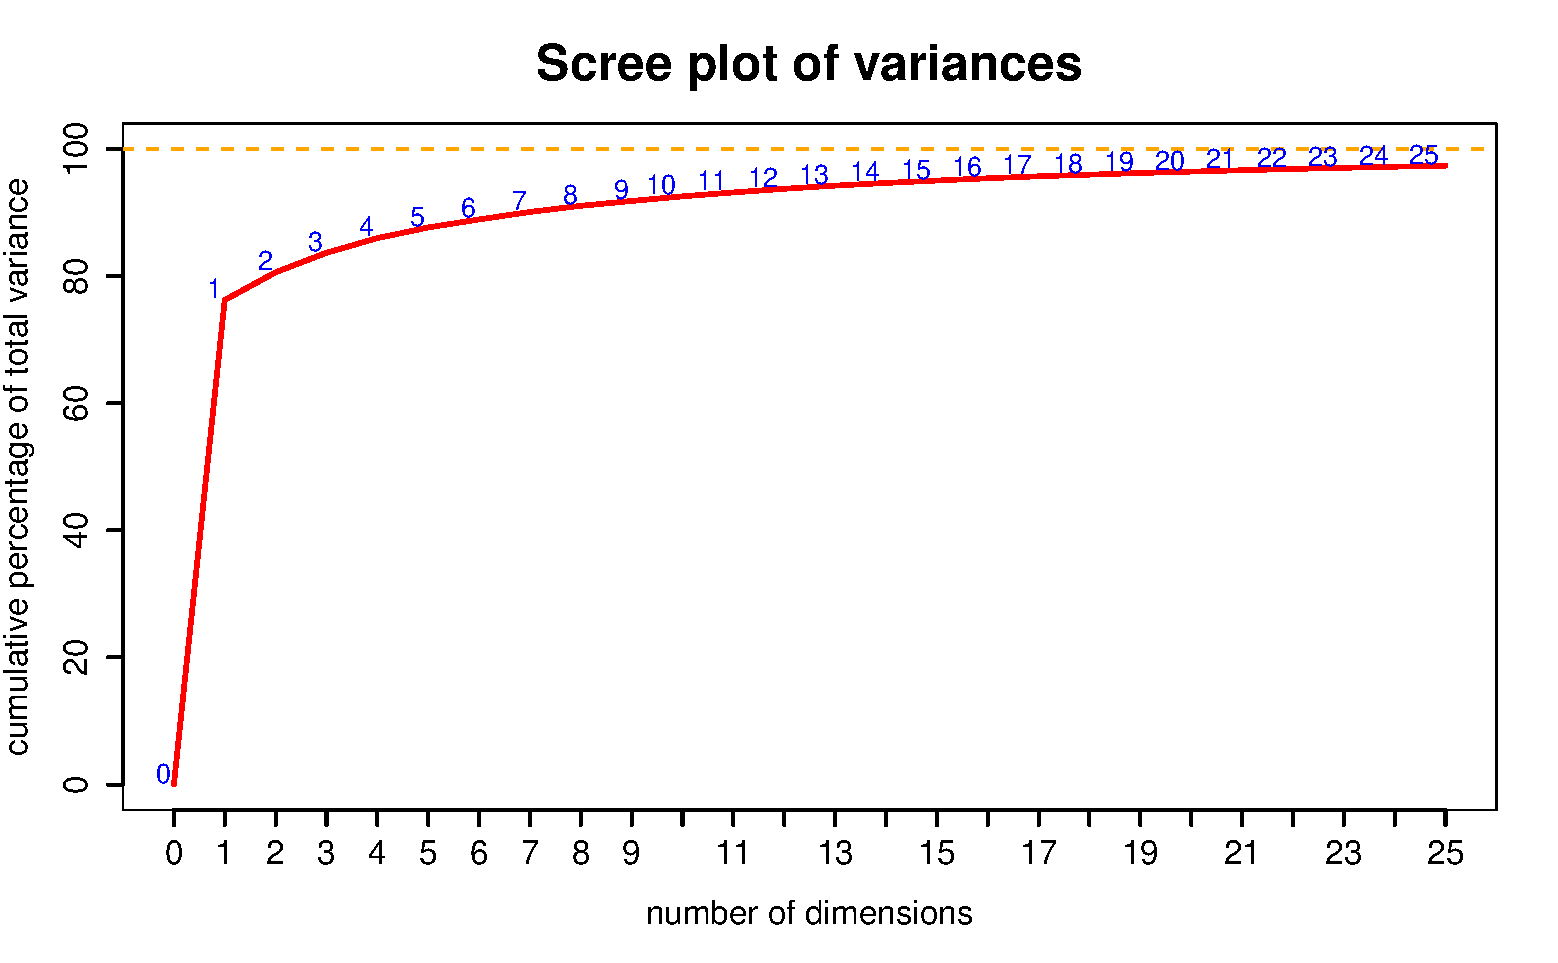
\includegraphics[scale=0.5]{screeAll.pdf}
%\caption{Screeplot showing explained variance against dimension number showing that the first PC captures about 80\% of the observed variance.} 
%\label{F:PCAScree}
%\end{center}
%\end{figure}
%
%\begin{figure}[H]
%\begin{center}
%\includegraphics[width=\textwidth]{ldaTypeScalings.pdf}
%\caption{The scalings for LDA based discrimination of lupus sources.} 
% \label{F:LDATypeScalings}
%\end{center}
%\end{figure}

%\subsection*{Other Work}

%\subsubsection{Randomisation Test}
%As a preliminary measure the difference in gene expression levels between patients and controls in the training dataset was assessed using a randomisation test with \gls{pFDR} \cite{pfdr} to control the false discovery rate. The analysis was consistant with the $limma$ based empirical bayes analysis and provided overwhelming evidence that many genes have different expression levels  in patients and controls (see Figure \ref{F:PFDR}). The randomisation test was based on MAS6001, Project 3 brief and reused my code from my project submission. The following algorithm was used:
%
%\begin{enumerate}
%\item Rank the patients by gene expression level and take the top 25\%, rank the controls by gene expression and take the top 25%.
%\item Calculate a t-statistic using the pooled variance.
%\item Repeat the above taking the top 50% and then the top 75\%.
%\item Do the same but with the lower 25\%, 50\% and 75\% in each group.
%\item Calculate the maximum of the absolute values of the six test statistics in 1-4 above.
%\item Randomly relabel the cases and controls and calculate the largest of the six t statistics.
%\item Repeat this lots of times.
%\item Calculate the $p$-value as the proportion of times that the maximum t statistic when the case control labels are mixed up exceeds the the maximum $T$ statistic in the original data.
%\item Do the above for each gene.
%\item Compare the $p$-value for each gene with some adjusted $p$-value taking into account number of tests done.
%\end{enumerate}
%
%
%\begin{figure}[H]
%\begin{center}
%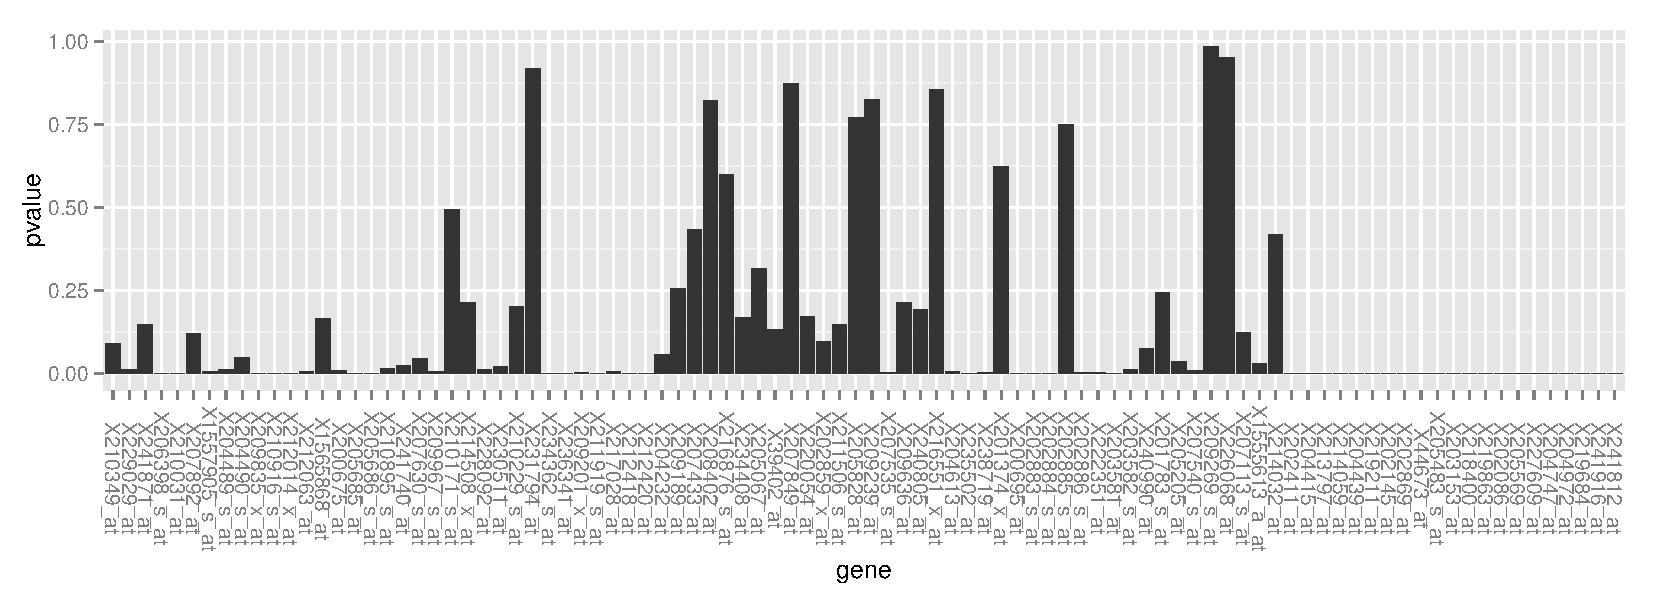
\includegraphics[width=\textwidth]{pfdr.pdf}
%\caption{Bar chart of $p$-values from $T$-tests testing the difference of gene expression levels between patients and controls. pFDR suggests that 43 are significant at the 1\% level,
%58 at the 5\% level and 63 at the 10\% level.} 
%\label{F:PFDR}
%\end{center}
%\end{figure}

%\subsubsection{Random Forest}
%Random Forests are a form of tree based supervised learning used in classification and regression problems. An attractive feature of random forests is their capacity to capture non-linear relationships between explanatory variables and their relative importance in predicting a response. Random forests gave very poor classification performance with a misclassification rate of 0.61 for controls.
%
%\subsubsection{Projection Pursuit}
%Exploratory projection pursuit is a form of dimension reduction that measures information as a departure from Normality as measured by a statistic called kurtosis. Therefore it may have greater capacity to handle non-linear associations than either PCA or LDA. Exploratory projection pursuit was also performed and appeared more capable of separating lupus patients and controls than LDA suggesting that non-linear effects may also be at play (see Figure \ref{F:PP}). While projection pursuit provided an interesting low dimensional view of the data a drawback is that interpretation in terms of gene expression is difficult.


%\begin{figure}[h]
%\begin{center}
%\includegraphics[width=\textwidth]{pp.JPG}
%\caption{Screenshot of 2D entropy based projection pursuit performed using GGobi. Projection pursuit appears better able to discriminate between lupus patients (yellow) and controls (purple), suggesting that non-linear relationships may be important.}
%\label{F:PP}
%\end{center}
%\end{figure}

%\section{Clustering}
%Clustering methods aim to separate the data into a set of distinguishable groups based on some distance metric. Clustering was used to try to identify groups of related genes based on the non-linear part of association which was converted into a dissimilarity metric by subtracting one. The aim was to try to identify if genes cluster into distinct groups that differ between lupus patients and controls. 
%
%Agglomerative, divisive and fixed clustering was explored using the functions $agnes$, $diana$ and $pam$ from the R package $cluster$ \cite{cluster}. Each clustering algorithm yielded a coefficient measuring the amount of clustering structure found and was in turn used to aid in model assessment.
%
%Hierarchical clustering attempts to create a hierarchy of groups from the given dataset. Agglomerative clustering works by successively amalgamating variables into groups while divisive clustering starts with one large group and successively divides it. Average linkage (the distance between cluster centroids) was used for the clustering process but other methods exist also.  
%
%%The results are shown in Figure \ref{F:dendroMinusR} but are somewhat inconclusive. There appears to be more clustering structure in controls than lupus patients as measured by the divisive coefficient. The heights suggest that both groups form many clusters (more so in controls) of quite distinct genes. However agglomerative clustering and fixed clustering yielded quite different results hence the cautionary not by \citet{MASS} suggesting that divisive clustering is a useful technique for discovering the major groups within a dataset but cautions against over interpreting dendrograms seems prudent.
%
%The divisive coefficient of 0.97 for each group suggests taht a lot of clustering structure was found. Based on the dendrogram heights it would appear that Lupus patients fall into around four clusters while controls have around six or seven clusters.
%
%\begin{enumerate}
%\item \textit{Use a more formal estimate such as the gap statistic for estimating cluster number.
%\item See how $MIC$and $dcor$ cluster.
%\item By subtract $A$from $R^2$ I ended up with some negative values so had to use absolute values to construct the dissimilarity matrix. This may be misleading or just wrong.
%\item Try cutting the dendrograms at selected heights, take representative genes and fit smoothing lines to pairwise plots to assess non-linearity if any.
%\item My intent is to use the clusters to try to find representative functional forms for pairwise associations and then maybe use these as a basis for non-linear regression or some other hypothesis test. Perhaps splines might be better suited for this.
%\item Try clustering based on residual association.}
%\end{enumerate}
%
%\begin{figure}[h]
%\begin{center}
%\includegraphics[width=\textwidth]{Adendro.pdf}
%\caption{A possible of gene expression for lupus patients and controls. The dendrograms are based on non-linear dissimilarity ($1-abs(A - R^2)$) using divisive clustering.} 
%\label{F:dendroMinusR}
%\end{center}
%\end{figure}

\chapter{Results from the Test Data}

\section{Bland-Altman Plots}
\begin{figure}[H]
\begin{center}
\includegraphics[width=\textwidth]{big2wayBA}
\caption{Bland-Altman plots comparing each association measure separately for controls and lupus patients on the test dataset.} 
\label{F:ba2way}
\end{center}
\end{figure}

\newpage
\section{Differentially expressed genes in the test dataset}


\begin{footnotesize}
\begin{longtable}{|>{}m{1cm} |>{}m{2cm} | >{}m{5cm}| >{}m{4cm} | }
  \hline
\textbf{Rank} & \textbf{Probe No} & \textbf{Probe ID} & \textbf{Log Fold Change}  \\ \hline
1 & 11860 & 202411\_at & 3.55 \\ 
  2 & 13887 & 204439\_at & 2.98 \\ 
  3 & 23359 & 214059\_at & 2.84 \\ 
  4 & 23753 & 214453\_s\_at & 2.65 \\ 
  5 & 51875 & 242625\_at & 2.62 \\ 
  6 & 23098 & 213797\_at & 2.56 \\ 
  7 & 33848 & 224588\_at & 2.41 \\ 
  8 & 49229 & 239979\_at & 2.12 \\ 
  9 & 36926 & 227671\_at & 2.00 \\ 
  10 & 28804 & 219519\_s\_at & 1.99 \\ 
  11 & 31009 & 221728\_x\_at & 1.95 \\ 
  12 & 27686 & 218400\_at & 1.94 \\ 
  13 & 35958 & 226702\_at & 1.93 \\ 
  14 & 14931 & 205483\_s\_at & 1.90 \\ 
  15 & 12602 & 203153\_at & 1.86 \\ 
  16 & 33850 & 224590\_at & 1.85 \\ 
  17 & 36864 & 227609\_at & 1.85 \\ 
  18 & 23518 & 214218\_s\_at & 1.83 \\ 
  19 & 44526 & 235276\_at & 1.76 \\ 
  20 & 21724 & 212418\_at & 1.76 \\ 
  21 & 29148 & 219863\_at & 1.75 \\ 
  22 & 11594 & 202145\_at & 1.73 \\ 
  23 & 11535 & 202086\_at & 1.69 \\ 
  24 & 28496 & 219211\_at & 1.69 \\ 
  25 & 37872 & 228617\_at & 1.68 \\ 
  26 & 14195 & 204747\_at & 1.68 \\ 
  27 & 40943 & 231688\_at & 1.61 \\ 
  28 & 51484 & 242234\_at & 1.56 \\ 
  29 & 16774 & 207329\_at & 1.56 \\ 
  30 & 15000 & 205552\_s\_at & 1.56 \\ 
  31 & 51166 & 241916\_at & 1.55 \\ 
  32 & 15017 & 205569\_at & 1.53 \\ 
  33 & 14420 & 204972\_at & 1.52 \\ 
  34 & 12318 & 202869\_at & 1.52 \\ 
  35 & 54649 & AFFX-r2-Bs-dap-3\_at & 1.51 \\ 
  36 & 28271 & 218986\_s\_at & 1.51 \\ 
  37 & 44407 & 235157\_at & 1.50 \\ 
  38 & 31435 & 222154\_s\_at & 1.47 \\ 
  39 & 33849 & 224589\_at & 1.40 \\ 
  40 & 32876 & 223599\_at & 1.39 \\ 
  41 & 51119 & 241869\_at & 1.38 \\ 
  42 & 42677 & 233425\_at & 1.36 \\ 
  43 & 37471 & 228216\_at & 1.35 \\ 
  44 & 39291 & 230036\_at & 1.34 \\ 
  45 & 28969 & 219684\_at & 1.34 \\ 
  46 & 39569 & 230314\_at & 1.34 \\ 
  47 & 22074 & 212768\_s\_at & 1.32 \\ 
  48 & 47993 & 238743\_at & 1.32 \\ 
  49 & 51270 & 242020\_s\_at & 1.32 \\ 
  50 & 14451 & 205003\_at & 1.32 \\ 
  51 & 11000 & 201551\_s\_at & 1.31 \\ 
  52 & 54623 & AFFX-DapX-3\_at & 1.30 \\ 
  53 & 40710 & 231455\_at & 1.30 \\ 
  54 & 38705 & 229450\_at & 1.29 \\ 
  55 & 12724 & 203276\_at & 1.28 \\ 
  56 & 28892 & 219607\_s\_at & 1.27 \\ 
  57 & 51062 & 241812\_at & 1.27 \\ 
  58 & 10435 & 200986\_at & 1.27 \\ 
  59 & 22596 & 213294\_at & 1.26 \\ 
  60 & 52521 & 243271\_at & 1.25 \\ 
  61 & 54404 & 44673\_at & 1.22 \\ 
  62 & 28637 & 219352\_at & 1.22 \\ 
  63 & 28494 & 219209\_at & 1.21 \\ 
  64 & 17856 & 208436\_s\_at & 1.21 \\ 
  65 & 35859 & 226603\_at & 1.20 \\ 
  66 & 28347 & 219062\_s\_at & 1.19 \\ 
  67 & 23954 & 214657\_s\_at & 1.19 \\ 
  68 & 11467 & 202018\_s\_at & 1.19 \\ 
  69 & 13043 & 203595\_s\_at & 1.18 \\ 
  70 & 15108 & 205660\_at & 1.18 \\ 
  71 & 2348 & 1555464\_at & 1.17 \\ 
  72 & 11879 & 202430\_s\_at & 1.17 \\ 
  73 & 16123 & 206676\_at & 1.17 \\ 
  74 & 22278 & 212974\_at & 1.16 \\ 
  75 & 1523 & 1554376\_s\_at & 1.16 \\ 
  76 & 11895 & 202446\_s\_at & 1.14 \\ 
  77 & 52713 & 243463\_s\_at & 1.14 \\ 
  78 & 13863 & 204415\_at & 1.14 \\ 
  79 & 36013 & 226757\_at & 1.13 \\ 
  80 & 16000 & 206553\_at & 1.12 \\ 
  81 & 13044 & 203596\_s\_at & 1.11 \\ 
  82 & 46676 & 237426\_at & 1.11 \\ 
  83 & 2177 & 1555247\_a\_at & 1.11 \\ 
  84 & 17244 & 207802\_at & 1.11 \\ 
  85 & 53074 & 243824\_at & 1.10 \\ 
  86 & 4877 & 1559585\_at & 1.10 \\ 
  87 & 32499 & 223220\_s\_at & 1.10 \\ 
  88 & 40855 & 231600\_at & 1.10 \\ 
  89 & 4017 & 1558011\_at & 1.09 \\ 
  90 & 54651 & AFFX-r2-Bs-dap-M\_at & 1.09 \\ 
  91 & 45473 & 236223\_s\_at & 1.09 \\ 
  92 & 10372 & 200923\_at & 1.08 \\ 
  93 & 13981 & 204533\_at & 1.08 \\ 
  94 & 11719 & 202270\_at & 1.07 \\ 
  95 & 20178 & 210797\_s\_at & 1.07 \\ 
  96 & 53038 & 243788\_at & 1.07 \\ 
  97 & 33496 & 224225\_s\_at & 1.07 \\ 
  98 & 44362 & 235112\_at & 1.06 \\ 
  99 & 28018 & 218733\_at & 1.06 \\ 
  100 & 45474 & 236224\_at & 1.06 \\ 
  101 & 37786 & 228531\_at & 1.05 \\ 
  102 & 49238 & 239988\_at & 1.05 \\ 
  103 & 36603 & 227347\_x\_at & 1.05 \\ 
  104 & 52148 & 242898\_at & 1.04 \\ 
  105 & 27829 & 218543\_s\_at & 1.04 \\ 
  106 & 47689 & 238439\_at & 1.04 \\ 
  107 & 53004 & 243754\_at & 1.04 \\ 
  108 & 41921 & 232666\_at & 1.04 \\ 
  109 & 36018 & 226762\_at & 1.04 \\ 
  110 & 17517 & 208087\_s\_at & 1.03 \\ 
  111 & 51310 & 242060\_x\_at & 1.03 \\ 
  112 & 41211 & 231956\_at & 1.03 \\ 
  113 & 28228 & 218943\_s\_at & 1.02 \\ 
  114 & 11339 & 201890\_at & 1.02 \\ 
  115 & 11952 & 202503\_s\_at & 1.01 \\ 
  116 & 2526 & 1555728\_a\_at & 1.01 \\ 
  117 & 37862 & 228607\_at & 1.01 \\ 
  118 & 33826 & 224566\_at & 1.01 \\ 
  119 & 31059 & 221778\_at & 1.00 \\ 
   \hline
\caption{Differentially expressed genes in the test dataset.} 
\label{T:bigDE}
\end{longtable}
\end{footnotesize}

\newpage
\section{Strong two-way associations in the test dataset}

\begin{footnotesize}
\begin{longtable}{ | >{}m{2cm}| >{}m{2cm} | >{}m{0.8cm}| >{}m{0.8cm} |>{}m{0.8cm}| >{}m{0.8cm} |>{}m{0.8cm}| >{}m{0.8cm} |>{}m{0.8cm}| >{}m{0.8cm} |}
  \hline
\textbf{$X_{Probe ID}$} & \textbf{$Y_{ProbeID}$}  & \textbf{$dcor$} & \textbf{$\sigma_{dcor}$} & \textbf{$R^2$} & \textbf{$\sigma_{R^2}$}& \textbf{$A$} & \textbf{$\sigma_{A}$} & \textbf{$MIC$} & \textbf{$\sigma_{MIC}$}  \\ 
  \hline
1552304\_at & 1552320\_a\_at & 0.938 & 0.008 & 0.835 & 0.021 & 0.934 & 0.011 & 0.962 & 0.020 \\ 
  1552320\_a\_at & 1552326\_a\_at & 0.928 & 0.010 & 0.806 & 0.030 & 0.929 & 0.011 & 0.944 & 0.029 \\ 
  1552275\_s\_at & 1552401\_a\_at & 0.926 & 0.011 & 0.821 & 0.022 & 0.930 & 0.012 & 0.869 & 0.034 \\ 
  1552256\_a\_at & 1552320\_a\_at & 0.925 & 0.007 & 0.820 & 0.013 & 0.938 & 0.009 & 0.947 & 0.025 \\ 
  1552275\_s\_at & 1552320\_a\_at & 0.924 & 0.008 & 0.815 & 0.016 & 0.940 & 0.010 & 0.950 & 0.027 \\ 
  1552326\_a\_at & 1552329\_at & 0.922 & 0.008 & 0.813 & 0.021 & 0.928 & 0.012 & 0.911 & 0.036 \\ 
  1552303\_a\_at & 1552320\_a\_at & 0.920 & 0.008 & 0.813 & 0.016 & 0.921 & 0.013 & 0.918 & 0.036 \\ 
  1552278\_a\_at & 1552301\_a\_at & 0.919 & 0.009 & 0.812 & 0.030 & 0.926 & 0.013 & 0.858 & 0.039 \\ 
  1552293\_at & 1552453\_a\_at & 0.919 & 0.008 & 0.809 & 0.015 & 0.930 & 0.011 & 0.943 & 0.031 \\ 
  1553658\_at & 1557551\_at & 0.916 & 0.008 & 0.802 & 0.016 & 0.908 & 0.015 & 0.951 & 0.039 \\ 
  1552398\_a\_at & 1552401\_a\_at & 0.916 & 0.010 & 0.803 & 0.022 & 0.913 & 0.014 & 0.865 & 0.034 \\ 
  1552401\_a\_at & 1552491\_at & 0.915 & 0.012 & 0.803 & 0.045 & 0.922 & 0.013 & 0.877 & 0.032 \\ 
  1552289\_a\_at & 201653\_at & 0.915 & 0.008 & 0.807 & 0.018 & 0.926 & 0.014 & 0.883 & 0.041 \\ 
  1552261\_at & 1552401\_a\_at & 0.915 & 0.010 & 0.787 & 0.027 & 0.916 & 0.015 & 0.850 & 0.037 \\ 
  117\_at & 1552401\_a\_at & 0.913 & 0.010 & 0.796 & 0.020 & 0.919 & 0.014 & 0.845 & 0.036 \\ 
  1552271\_at & 1552303\_a\_at & 0.913 & 0.010 & 0.807 & 0.025 & 0.921 & 0.014 & 0.889 & 0.040 \\ 
  1320\_at & 1552401\_a\_at & 0.912 & 0.011 & 0.803 & 0.021 & 0.928 & 0.012 & 0.851 & 0.036 \\ 
  1552320\_a\_at & 1552491\_at & 0.912 & 0.008 & 0.808 & 0.016 & 0.924 & 0.013 & 0.897 & 0.032 \\ 
  1552747\_a\_at & 1553015\_a\_at & 0.912 & 0.008 & 0.798 & 0.017 & 0.911 & 0.015 & 0.948 & 0.028 \\ 
  1552320\_a\_at & 1552338\_at & 0.912 & 0.009 & 0.807 & 0.015 & 0.922 & 0.013 & 0.906 & 0.032 \\ 
  1552293\_at & 227316\_at & 0.911 & 0.008 & 0.792 & 0.016 & 0.923 & 0.013 & 0.924 & 0.039 \\ 
  1320\_at & 1552325\_at & 0.910 & 0.008 & 0.781 & 0.015 & 0.922 & 0.014 & 0.895 & 0.038 \\ 
  1053\_at & 1552320\_a\_at & 0.910 & 0.008 & 0.771 & 0.016 & 0.941 & 0.009 & 0.971 & 0.018 \\ 
  1552293\_at & 1552327\_at & 0.910 & 0.009 & 0.796 & 0.018 & 0.931 & 0.012 & 0.863 & 0.038 \\ 
  1552271\_at & 1552320\_a\_at & 0.910 & 0.009 & 0.801 & 0.015 & 0.920 & 0.014 & 0.900 & 0.036 \\ 
  1552293\_at & 1552330\_at & 0.909 & 0.011 & 0.763 & 0.040 & 0.926 & 0.013 & 0.897 & 0.038 \\ 
  1007\_s\_at & 201653\_at & 0.909 & 0.009 & 0.806 & 0.019 & 0.928 & 0.013 & 0.882 & 0.040 \\ 
  1552264\_a\_at & 1552401\_a\_at & 0.908 & 0.013 & 0.776 & 0.028 & 0.915 & 0.014 & 0.846 & 0.035 \\ 
  1552283\_s\_at & 201653\_at & 0.908 & 0.009 & 0.800 & 0.016 & 0.925 & 0.014 & 0.861 & 0.039 \\ 
  1431\_at & 1552303\_a\_at & 0.908 & 0.010 & 0.799 & 0.020 & 0.920 & 0.014 & 0.861 & 0.042 \\ 
  1552274\_at & 1552453\_a\_at & 0.908 & 0.008 & 0.794 & 0.014 & 0.932 & 0.011 & 0.949 & 0.024 \\ 
  121\_at & 1552401\_a\_at & 0.908 & 0.009 & 0.766 & 0.018 & 0.912 & 0.016 & 0.839 & 0.035 \\ 
  1552747\_a\_at & 1553603\_s\_at & 0.907 & 0.008 & 0.798 & 0.019 & 0.900 & 0.017 & 0.929 & 0.031 \\ 
  1552289\_a\_at & 1552338\_at & 0.907 & 0.010 & 0.770 & 0.018 & 0.931 & 0.011 & 0.866 & 0.037 \\ 
  1552280\_at & 1552320\_a\_at & 0.907 & 0.010 & 0.785 & 0.017 & 0.919 & 0.014 & 0.919 & 0.038 \\ 
  1552322\_at & 1552394\_a\_at & 0.907 & 0.010 & 0.806 & 0.016 & 0.927 & 0.012 & 0.865 & 0.043 \\ 
  1552293\_at & 1552349\_a\_at & 0.907 & 0.009 & 0.800 & 0.017 & 0.935 & 0.011 & 0.881 & 0.032 \\ 
  1552264\_a\_at & 1552320\_a\_at & 0.906 & 0.010 & 0.766 & 0.022 & 0.923 & 0.013 & 0.909 & 0.033 \\ 
  1552747\_a\_at & 1553508\_at & 0.906 & 0.009 & 0.787 & 0.017 & 0.895 & 0.017 & 0.931 & 0.029 \\ 
  1552278\_a\_at & 1552320\_a\_at & 0.905 & 0.009 & 0.788 & 0.018 & 0.922 & 0.013 & 0.910 & 0.032 \\ 
  1552261\_at & 1552320\_a\_at & 0.905 & 0.008 & 0.766 & 0.017 & 0.924 & 0.012 & 0.922 & 0.030 \\ 
  1552274\_at & 201030\_x\_at & 0.904 & 0.011 & 0.798 & 0.019 & 0.923 & 0.013 & 0.872 & 0.037 \\ 
  1552276\_a\_at & 1552644\_a\_at & 0.904 & 0.009 & 0.788 & 0.021 & 0.923 & 0.013 & 0.917 & 0.033 \\ 
  1552289\_a\_at & 1552384\_a\_at & 0.904 & 0.010 & 0.767 & 0.020 & 0.931 & 0.012 & 0.862 & 0.037 \\ 
  1431\_at & 1552453\_a\_at & 0.904 & 0.009 & 0.798 & 0.014 & 0.935 & 0.010 & 0.927 & 0.030 \\ 
  1487\_at & 1552415\_a\_at & 0.904 & 0.011 & 0.803 & 0.020 & 0.922 & 0.014 & 0.865 & 0.042 \\ 
  1320\_at & 1552360\_a\_at & 0.904 & 0.010 & 0.786 & 0.016 & 0.924 & 0.013 & 0.855 & 0.045 \\ 
  1320\_at & 1552320\_a\_at & 0.903 & 0.009 & 0.784 & 0.015 & 0.928 & 0.012 & 0.908 & 0.036 \\ 
  1552274\_at & 227316\_at & 0.903 & 0.009 & 0.788 & 0.016 & 0.929 & 0.012 & 0.911 & 0.041 \\ 
  1552304\_at & 227316\_at & 0.902 & 0.008 & 0.761 & 0.019 & 0.914 & 0.015 & 0.927 & 0.033 \\ 
  1552320\_a\_at & 1553093\_a\_at & 0.902 & 0.010 & 0.799 & 0.020 & 0.896 & 0.016 & 0.896 & 0.038 \\ 
  1552276\_a\_at & 1552415\_a\_at & 0.902 & 0.009 & 0.786 & 0.015 & 0.920 & 0.014 & 0.884 & 0.045 \\ 
  1552293\_at & 1552332\_at & 0.902 & 0.012 & 0.787 & 0.027 & 0.927 & 0.013 & 0.843 & 0.035 \\ 
  1552320\_a\_at & 1553069\_at & 0.902 & 0.011 & 0.798 & 0.019 & 0.898 & 0.015 & 0.890 & 0.036 \\ 
  1007\_s\_at & 1320\_at & 0.902 & 0.011 & 0.796 & 0.018 & 0.922 & 0.015 & 0.853 & 0.044 \\ 
  1552320\_a\_at & 1552322\_at & 0.902 & 0.011 & 0.776 & 0.021 & 0.924 & 0.013 & 0.886 & 0.036 \\ 
  1552276\_a\_at & 1552790\_a\_at & 0.901 & 0.010 & 0.786 & 0.016 & 0.897 & 0.017 & 0.845 & 0.047 \\ 
   \hline
\caption{Bootstrap estimates of association of the 57 strong two-way associations present  in lupus patients but not in controls in the test dataset.} 
\label{T:bigAE}
\end{longtable}
\end{footnotesize}


%\chapter{Poster}
%Below is the poster accompanying the project. 
%\input{JRochePoster.tex}

\end{document}